% Generated by Sphinx.
\def\sphinxdocclass{report}
\documentclass[letterpaper,10pt,english]{sphinxmanual}
\usepackage[utf8]{inputenc}
\DeclareUnicodeCharacter{00A0}{\nobreakspace}
\usepackage{cmap}
\usepackage[T1]{fontenc}
\usepackage{babel}
\usepackage{times}
\usepackage[Bjarne]{fncychap}
\usepackage{longtable}
\usepackage{sphinx}
\usepackage{multirow}


\title{UAH Bit Vault Documentation}
\date{April 24, 2016}
\release{1.0}
\author{Timothy Wilkins}
\newcommand{\sphinxlogo}{}
\renewcommand{\releasename}{Release}
\makeindex

\makeatletter
\def\PYG@reset{\let\PYG@it=\relax \let\PYG@bf=\relax%
    \let\PYG@ul=\relax \let\PYG@tc=\relax%
    \let\PYG@bc=\relax \let\PYG@ff=\relax}
\def\PYG@tok#1{\csname PYG@tok@#1\endcsname}
\def\PYG@toks#1+{\ifx\relax#1\empty\else%
    \PYG@tok{#1}\expandafter\PYG@toks\fi}
\def\PYG@do#1{\PYG@bc{\PYG@tc{\PYG@ul{%
    \PYG@it{\PYG@bf{\PYG@ff{#1}}}}}}}
\def\PYG#1#2{\PYG@reset\PYG@toks#1+\relax+\PYG@do{#2}}

\expandafter\def\csname PYG@tok@gd\endcsname{\def\PYG@tc##1{\textcolor[rgb]{0.63,0.00,0.00}{##1}}}
\expandafter\def\csname PYG@tok@gu\endcsname{\let\PYG@bf=\textbf\def\PYG@tc##1{\textcolor[rgb]{0.50,0.00,0.50}{##1}}}
\expandafter\def\csname PYG@tok@gt\endcsname{\def\PYG@tc##1{\textcolor[rgb]{0.00,0.27,0.87}{##1}}}
\expandafter\def\csname PYG@tok@gs\endcsname{\let\PYG@bf=\textbf}
\expandafter\def\csname PYG@tok@gr\endcsname{\def\PYG@tc##1{\textcolor[rgb]{1.00,0.00,0.00}{##1}}}
\expandafter\def\csname PYG@tok@cm\endcsname{\let\PYG@it=\textit\def\PYG@tc##1{\textcolor[rgb]{0.25,0.50,0.56}{##1}}}
\expandafter\def\csname PYG@tok@vg\endcsname{\def\PYG@tc##1{\textcolor[rgb]{0.73,0.38,0.84}{##1}}}
\expandafter\def\csname PYG@tok@m\endcsname{\def\PYG@tc##1{\textcolor[rgb]{0.13,0.50,0.31}{##1}}}
\expandafter\def\csname PYG@tok@mh\endcsname{\def\PYG@tc##1{\textcolor[rgb]{0.13,0.50,0.31}{##1}}}
\expandafter\def\csname PYG@tok@cs\endcsname{\def\PYG@tc##1{\textcolor[rgb]{0.25,0.50,0.56}{##1}}\def\PYG@bc##1{\setlength{\fboxsep}{0pt}\colorbox[rgb]{1.00,0.94,0.94}{\strut ##1}}}
\expandafter\def\csname PYG@tok@ge\endcsname{\let\PYG@it=\textit}
\expandafter\def\csname PYG@tok@vc\endcsname{\def\PYG@tc##1{\textcolor[rgb]{0.73,0.38,0.84}{##1}}}
\expandafter\def\csname PYG@tok@il\endcsname{\def\PYG@tc##1{\textcolor[rgb]{0.13,0.50,0.31}{##1}}}
\expandafter\def\csname PYG@tok@go\endcsname{\def\PYG@tc##1{\textcolor[rgb]{0.20,0.20,0.20}{##1}}}
\expandafter\def\csname PYG@tok@cp\endcsname{\def\PYG@tc##1{\textcolor[rgb]{0.00,0.44,0.13}{##1}}}
\expandafter\def\csname PYG@tok@gi\endcsname{\def\PYG@tc##1{\textcolor[rgb]{0.00,0.63,0.00}{##1}}}
\expandafter\def\csname PYG@tok@gh\endcsname{\let\PYG@bf=\textbf\def\PYG@tc##1{\textcolor[rgb]{0.00,0.00,0.50}{##1}}}
\expandafter\def\csname PYG@tok@ni\endcsname{\let\PYG@bf=\textbf\def\PYG@tc##1{\textcolor[rgb]{0.84,0.33,0.22}{##1}}}
\expandafter\def\csname PYG@tok@nl\endcsname{\let\PYG@bf=\textbf\def\PYG@tc##1{\textcolor[rgb]{0.00,0.13,0.44}{##1}}}
\expandafter\def\csname PYG@tok@nn\endcsname{\let\PYG@bf=\textbf\def\PYG@tc##1{\textcolor[rgb]{0.05,0.52,0.71}{##1}}}
\expandafter\def\csname PYG@tok@no\endcsname{\def\PYG@tc##1{\textcolor[rgb]{0.38,0.68,0.84}{##1}}}
\expandafter\def\csname PYG@tok@na\endcsname{\def\PYG@tc##1{\textcolor[rgb]{0.25,0.44,0.63}{##1}}}
\expandafter\def\csname PYG@tok@nb\endcsname{\def\PYG@tc##1{\textcolor[rgb]{0.00,0.44,0.13}{##1}}}
\expandafter\def\csname PYG@tok@nc\endcsname{\let\PYG@bf=\textbf\def\PYG@tc##1{\textcolor[rgb]{0.05,0.52,0.71}{##1}}}
\expandafter\def\csname PYG@tok@nd\endcsname{\let\PYG@bf=\textbf\def\PYG@tc##1{\textcolor[rgb]{0.33,0.33,0.33}{##1}}}
\expandafter\def\csname PYG@tok@ne\endcsname{\def\PYG@tc##1{\textcolor[rgb]{0.00,0.44,0.13}{##1}}}
\expandafter\def\csname PYG@tok@nf\endcsname{\def\PYG@tc##1{\textcolor[rgb]{0.02,0.16,0.49}{##1}}}
\expandafter\def\csname PYG@tok@si\endcsname{\let\PYG@it=\textit\def\PYG@tc##1{\textcolor[rgb]{0.44,0.63,0.82}{##1}}}
\expandafter\def\csname PYG@tok@s2\endcsname{\def\PYG@tc##1{\textcolor[rgb]{0.25,0.44,0.63}{##1}}}
\expandafter\def\csname PYG@tok@vi\endcsname{\def\PYG@tc##1{\textcolor[rgb]{0.73,0.38,0.84}{##1}}}
\expandafter\def\csname PYG@tok@nt\endcsname{\let\PYG@bf=\textbf\def\PYG@tc##1{\textcolor[rgb]{0.02,0.16,0.45}{##1}}}
\expandafter\def\csname PYG@tok@nv\endcsname{\def\PYG@tc##1{\textcolor[rgb]{0.73,0.38,0.84}{##1}}}
\expandafter\def\csname PYG@tok@s1\endcsname{\def\PYG@tc##1{\textcolor[rgb]{0.25,0.44,0.63}{##1}}}
\expandafter\def\csname PYG@tok@gp\endcsname{\let\PYG@bf=\textbf\def\PYG@tc##1{\textcolor[rgb]{0.78,0.36,0.04}{##1}}}
\expandafter\def\csname PYG@tok@sh\endcsname{\def\PYG@tc##1{\textcolor[rgb]{0.25,0.44,0.63}{##1}}}
\expandafter\def\csname PYG@tok@ow\endcsname{\let\PYG@bf=\textbf\def\PYG@tc##1{\textcolor[rgb]{0.00,0.44,0.13}{##1}}}
\expandafter\def\csname PYG@tok@sx\endcsname{\def\PYG@tc##1{\textcolor[rgb]{0.78,0.36,0.04}{##1}}}
\expandafter\def\csname PYG@tok@bp\endcsname{\def\PYG@tc##1{\textcolor[rgb]{0.00,0.44,0.13}{##1}}}
\expandafter\def\csname PYG@tok@c1\endcsname{\let\PYG@it=\textit\def\PYG@tc##1{\textcolor[rgb]{0.25,0.50,0.56}{##1}}}
\expandafter\def\csname PYG@tok@kc\endcsname{\let\PYG@bf=\textbf\def\PYG@tc##1{\textcolor[rgb]{0.00,0.44,0.13}{##1}}}
\expandafter\def\csname PYG@tok@c\endcsname{\let\PYG@it=\textit\def\PYG@tc##1{\textcolor[rgb]{0.25,0.50,0.56}{##1}}}
\expandafter\def\csname PYG@tok@mf\endcsname{\def\PYG@tc##1{\textcolor[rgb]{0.13,0.50,0.31}{##1}}}
\expandafter\def\csname PYG@tok@err\endcsname{\def\PYG@bc##1{\setlength{\fboxsep}{0pt}\fcolorbox[rgb]{1.00,0.00,0.00}{1,1,1}{\strut ##1}}}
\expandafter\def\csname PYG@tok@kd\endcsname{\let\PYG@bf=\textbf\def\PYG@tc##1{\textcolor[rgb]{0.00,0.44,0.13}{##1}}}
\expandafter\def\csname PYG@tok@ss\endcsname{\def\PYG@tc##1{\textcolor[rgb]{0.32,0.47,0.09}{##1}}}
\expandafter\def\csname PYG@tok@sr\endcsname{\def\PYG@tc##1{\textcolor[rgb]{0.14,0.33,0.53}{##1}}}
\expandafter\def\csname PYG@tok@mo\endcsname{\def\PYG@tc##1{\textcolor[rgb]{0.13,0.50,0.31}{##1}}}
\expandafter\def\csname PYG@tok@mi\endcsname{\def\PYG@tc##1{\textcolor[rgb]{0.13,0.50,0.31}{##1}}}
\expandafter\def\csname PYG@tok@kn\endcsname{\let\PYG@bf=\textbf\def\PYG@tc##1{\textcolor[rgb]{0.00,0.44,0.13}{##1}}}
\expandafter\def\csname PYG@tok@o\endcsname{\def\PYG@tc##1{\textcolor[rgb]{0.40,0.40,0.40}{##1}}}
\expandafter\def\csname PYG@tok@kr\endcsname{\let\PYG@bf=\textbf\def\PYG@tc##1{\textcolor[rgb]{0.00,0.44,0.13}{##1}}}
\expandafter\def\csname PYG@tok@s\endcsname{\def\PYG@tc##1{\textcolor[rgb]{0.25,0.44,0.63}{##1}}}
\expandafter\def\csname PYG@tok@kp\endcsname{\def\PYG@tc##1{\textcolor[rgb]{0.00,0.44,0.13}{##1}}}
\expandafter\def\csname PYG@tok@w\endcsname{\def\PYG@tc##1{\textcolor[rgb]{0.73,0.73,0.73}{##1}}}
\expandafter\def\csname PYG@tok@kt\endcsname{\def\PYG@tc##1{\textcolor[rgb]{0.56,0.13,0.00}{##1}}}
\expandafter\def\csname PYG@tok@sc\endcsname{\def\PYG@tc##1{\textcolor[rgb]{0.25,0.44,0.63}{##1}}}
\expandafter\def\csname PYG@tok@sb\endcsname{\def\PYG@tc##1{\textcolor[rgb]{0.25,0.44,0.63}{##1}}}
\expandafter\def\csname PYG@tok@k\endcsname{\let\PYG@bf=\textbf\def\PYG@tc##1{\textcolor[rgb]{0.00,0.44,0.13}{##1}}}
\expandafter\def\csname PYG@tok@se\endcsname{\let\PYG@bf=\textbf\def\PYG@tc##1{\textcolor[rgb]{0.25,0.44,0.63}{##1}}}
\expandafter\def\csname PYG@tok@sd\endcsname{\let\PYG@it=\textit\def\PYG@tc##1{\textcolor[rgb]{0.25,0.44,0.63}{##1}}}

\def\PYGZbs{\char`\\}
\def\PYGZus{\char`\_}
\def\PYGZob{\char`\{}
\def\PYGZcb{\char`\}}
\def\PYGZca{\char`\^}
\def\PYGZam{\char`\&}
\def\PYGZlt{\char`\<}
\def\PYGZgt{\char`\>}
\def\PYGZsh{\char`\#}
\def\PYGZpc{\char`\%}
\def\PYGZdl{\char`\$}
\def\PYGZhy{\char`\-}
\def\PYGZsq{\char`\'}
\def\PYGZdq{\char`\"}
\def\PYGZti{\char`\~}
% for compatibility with earlier versions
\def\PYGZat{@}
\def\PYGZlb{[}
\def\PYGZrb{]}
\makeatother

\begin{document}

\maketitle
\tableofcontents
\phantomsection\label{index::doc}


Contents:


\chapter{User Guide}
\label{user_guide/user_guide:user-guide}\label{user_guide/user_guide::doc}\label{user_guide/user_guide:uah-fit-vault}\label{user_guide/user_guide:id1}\setbox0\vbox{
\begin{minipage}{0.95\linewidth}
\textbf{Table of Contents}

\medskip

\begin{itemize}
\item {} 
{\hyperref[user_guide/user_guide:user-guide]{User Guide}}
\begin{itemize}
\item {} 
{\hyperref[user_guide/user_guide:overview]{Overview}}

\item {} 
{\hyperref[user_guide/user_guide:how-to]{How-To}}

\end{itemize}

\end{itemize}
\end{minipage}}
\begin{center}\setlength{\fboxsep}{5pt}\shadowbox{\box0}\end{center}


\section{Overview}
\label{user_guide/user_guide:overview}
Here you can find all the documentation you will need to know how to do all the basic tasks that can be performed
through the UAH Bit Vault user interface.


\section{How-To}
\label{user_guide/user_guide:how-to}

\subsection{Account Management}
\label{user_guide/account_management::doc}\label{user_guide/account_management:account-management}\label{user_guide/account_management:id1}
Account management is a part of the system. Accounts may be created, deleted or edited. Follow the below TOC tree
to find details on each action for each account.

Contents:


\subsubsection{Account Creation}
\label{user_guide/account_creation::doc}\label{user_guide/account_creation:account-creation}\label{user_guide/account_creation:id1}\setbox0\vbox{
\begin{minipage}{0.95\linewidth}
\textbf{Table of Contents}

\medskip

\begin{itemize}
\item {} 
{\hyperref[user_guide/account_creation:account-creation]{Account Creation}}
\begin{itemize}
\item {} 
{\hyperref[user_guide/account_creation:physician-account]{Physician Account}}

\item {} 
{\hyperref[user_guide/account_creation:experiment-admin-account]{Experiment Admin Account}}

\item {} 
{\hyperref[user_guide/account_creation:patient-account]{Patient Account}}

\item {} 
{\hyperref[user_guide/account_creation:system-admin-account]{System Admin Account}}

\end{itemize}

\end{itemize}
\end{minipage}}
\begin{center}\setlength{\fboxsep}{5pt}\shadowbox{\box0}\end{center}

There are 4 types of accounts
\begin{itemize}
\item {} 
patient

\item {} 
physician

\item {} 
experiment admin

\item {} 
system admin

\end{itemize}


\paragraph{Physician Account}
\label{user_guide/account_creation:create-physician-account}\label{user_guide/account_creation:physician-account}
Physician accounts can be requested at the home/login page. Click on the ``Register as a new user'' button.

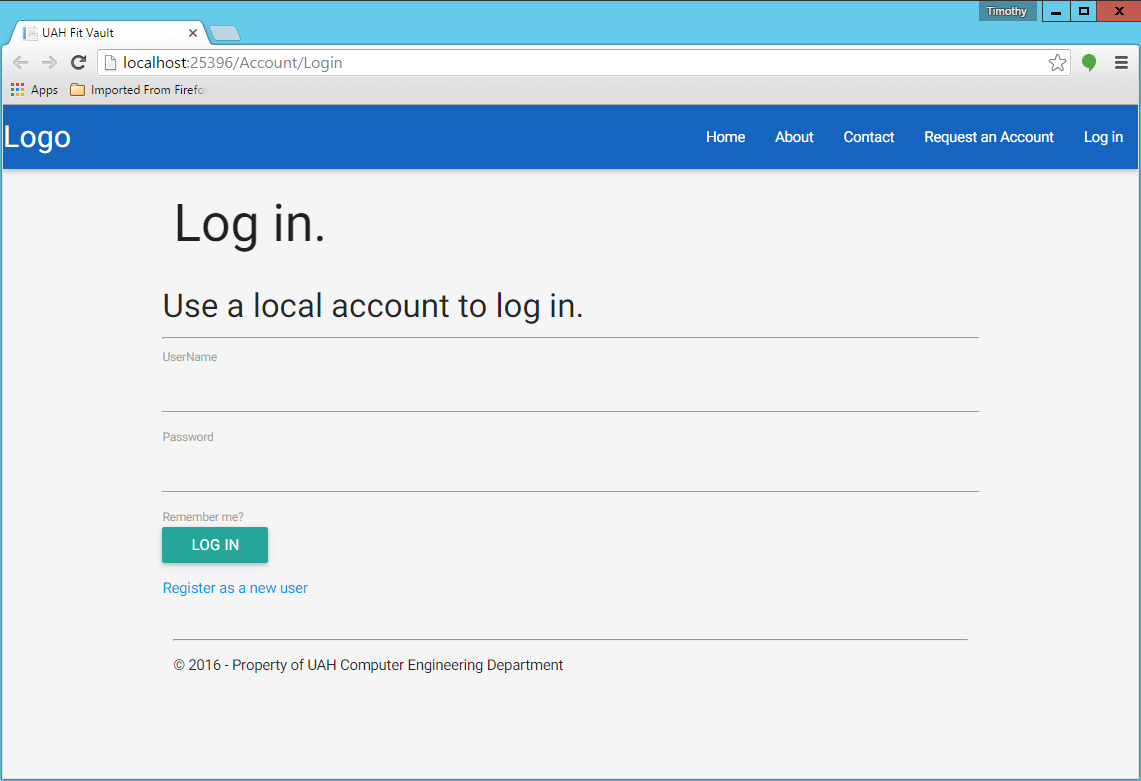
\includegraphics{login_screen.png}

This will redirect you to a form to fill out for you new physician account.

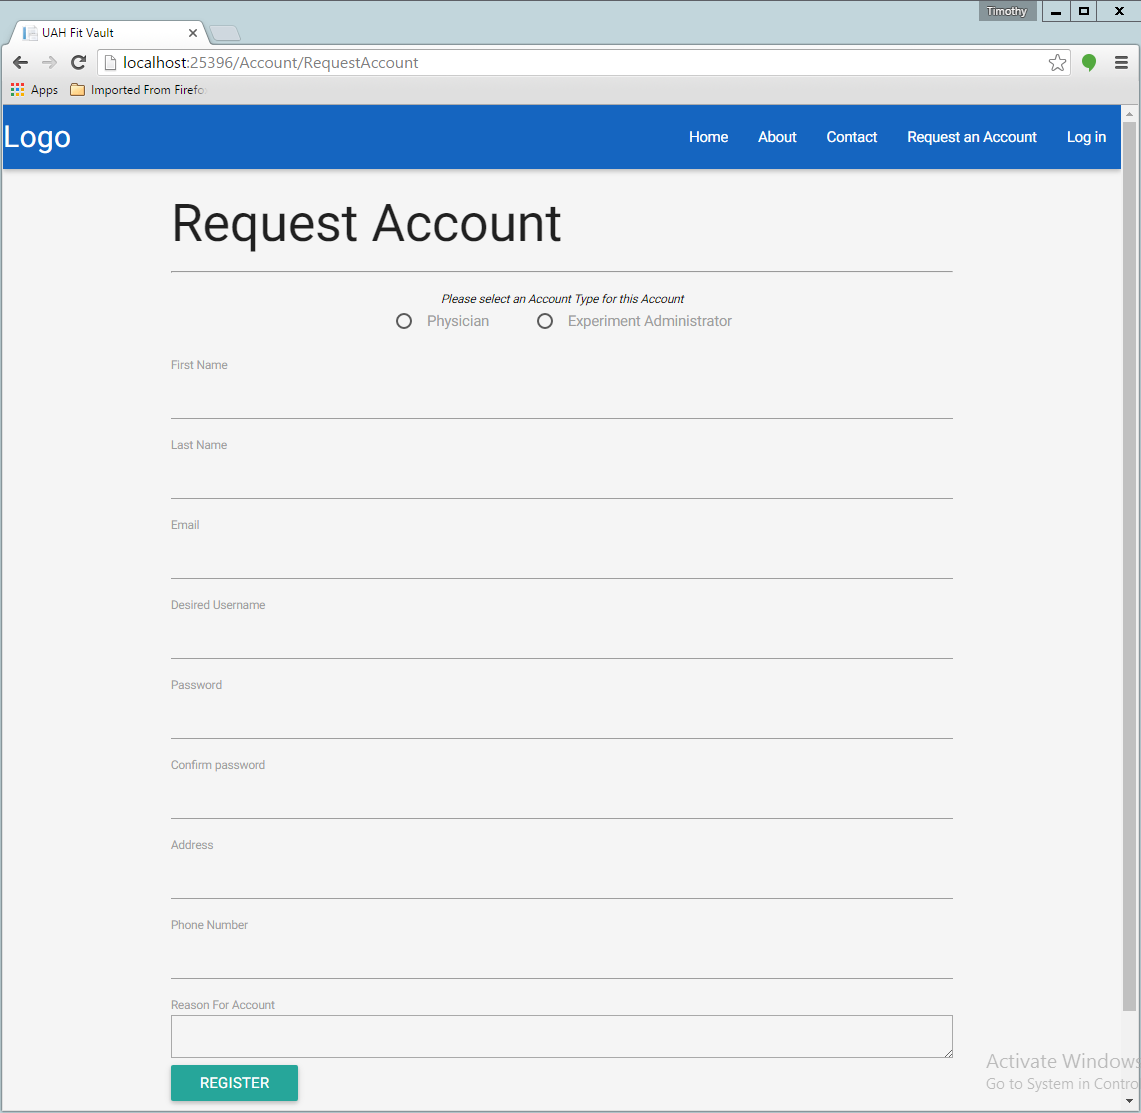
\includegraphics{request_account.png}

Once you have filled this out with the appropriate information and selected the ``Physician'' radio button at the top,
you are ready to submit your request. When you click submit you should be brought to a confirmation page.

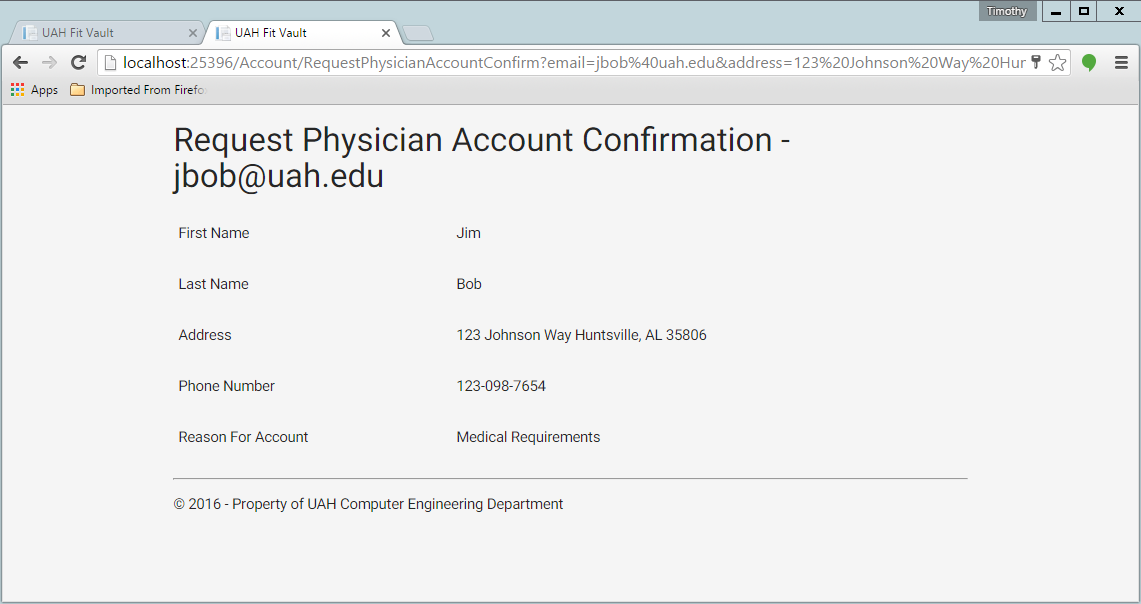
\includegraphics{request_account_confirmation.png}

You will not be able to login though until a system admin has approved your account.


\paragraph{Experiment Admin Account}
\label{user_guide/account_creation:experiment-admin-account}
Experiment Admin accounts are created the same way as the physician accounts. Just make sure to select the ``Experiment Administrator''
radio button at the top of the request account page instead of the ``Physician'' radio button.

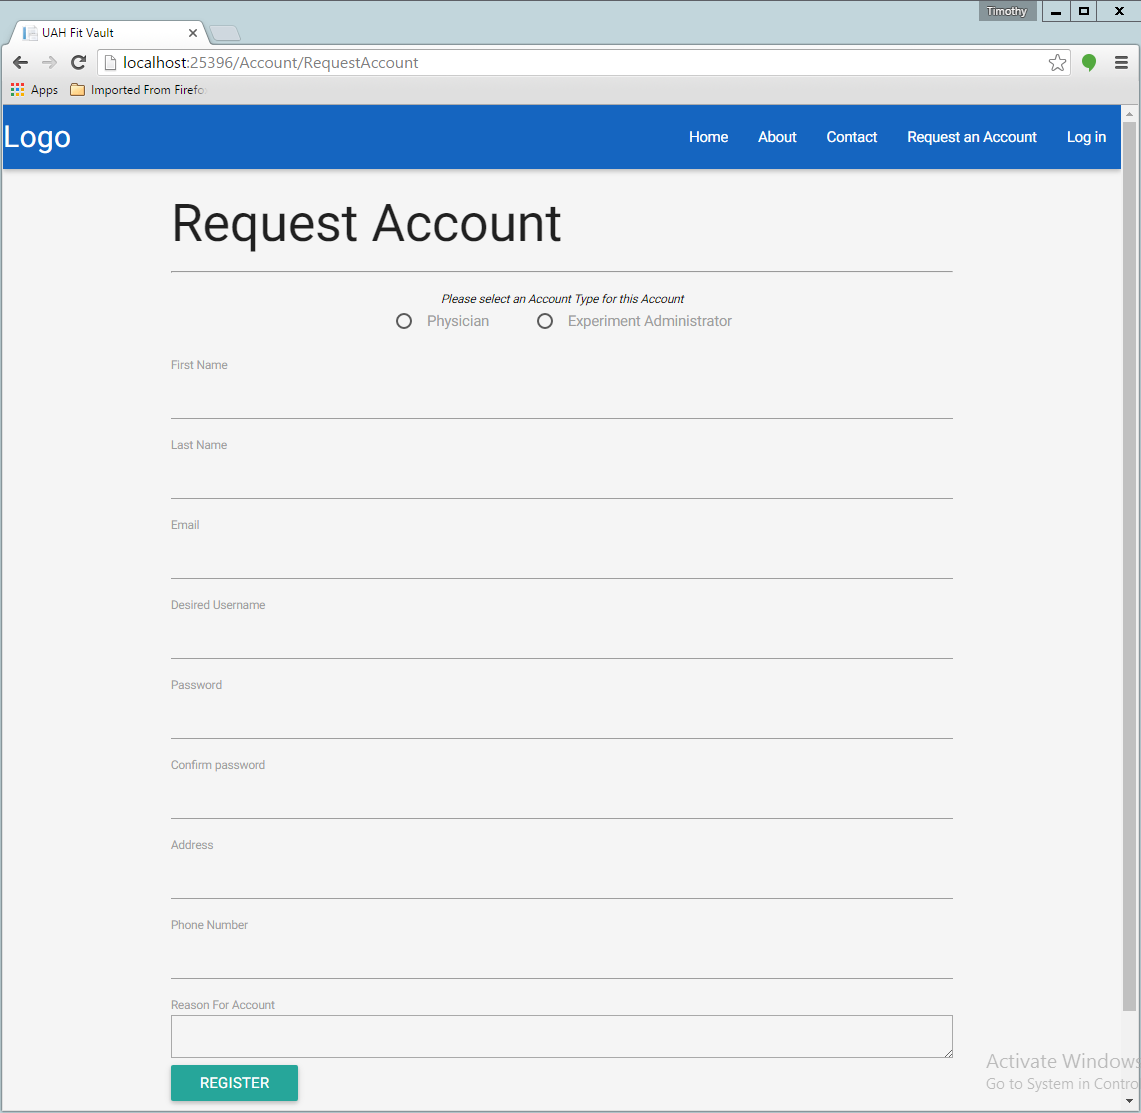
\includegraphics{request_account.png}


\paragraph{Patient Account}
\label{user_guide/account_creation:create-patient-account}\label{user_guide/account_creation:patient-account}
Patient accounts can only be created by their physician. From the physician account's home page click the ``CREATE PATIENT''
button at the top right of the screen.

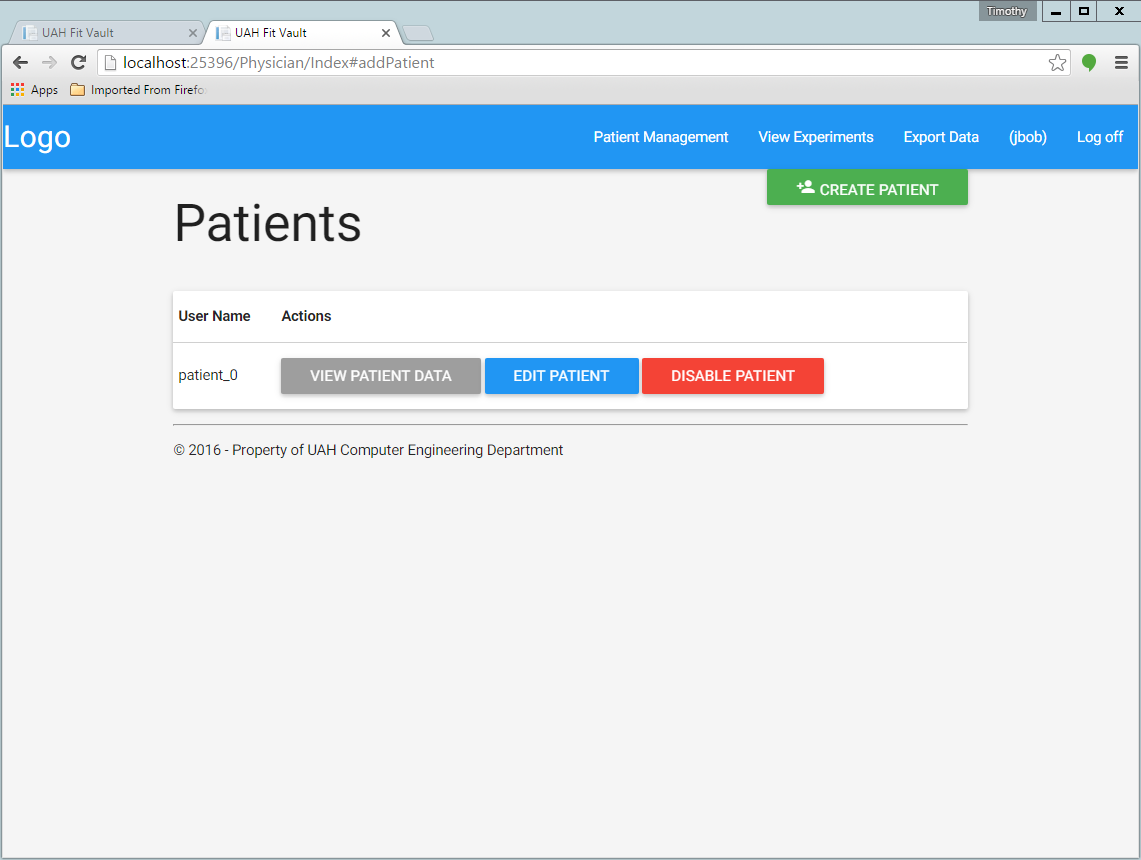
\includegraphics{patient_management.png}

A popup form should come up with all the information needed to create a patient account.

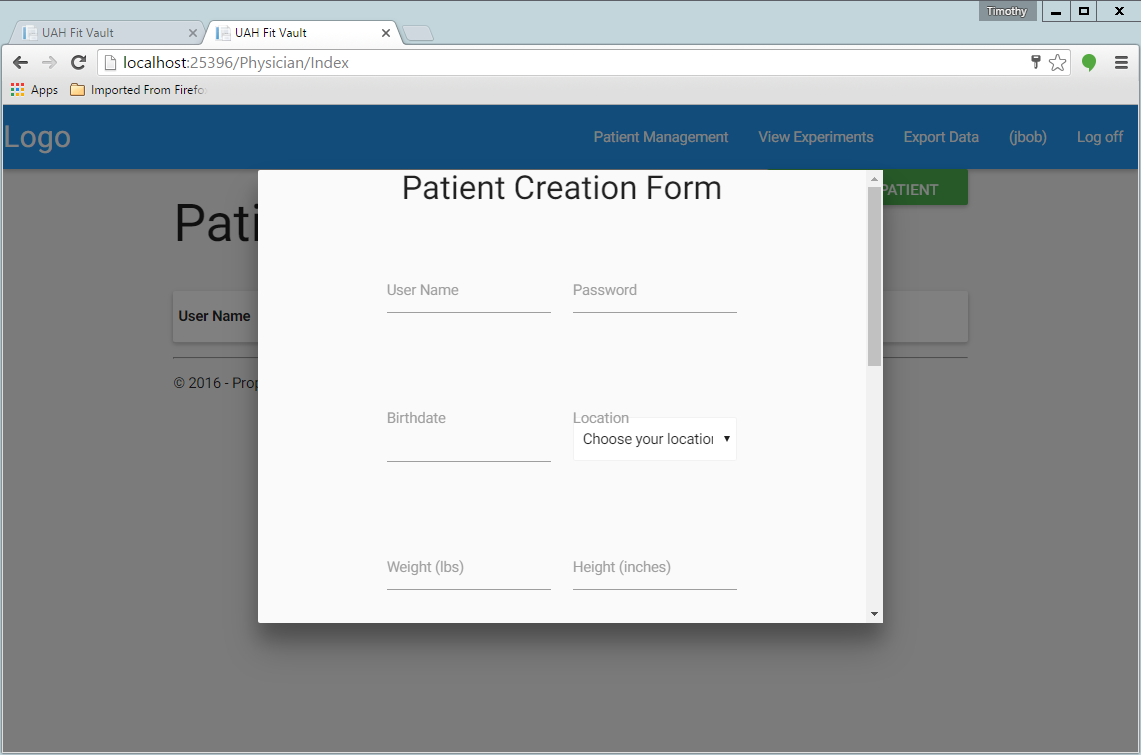
\includegraphics{create_patient.png}

After all the information has been filled out, you can click the submit button. If everthing worked, you should get a
confirmation page.

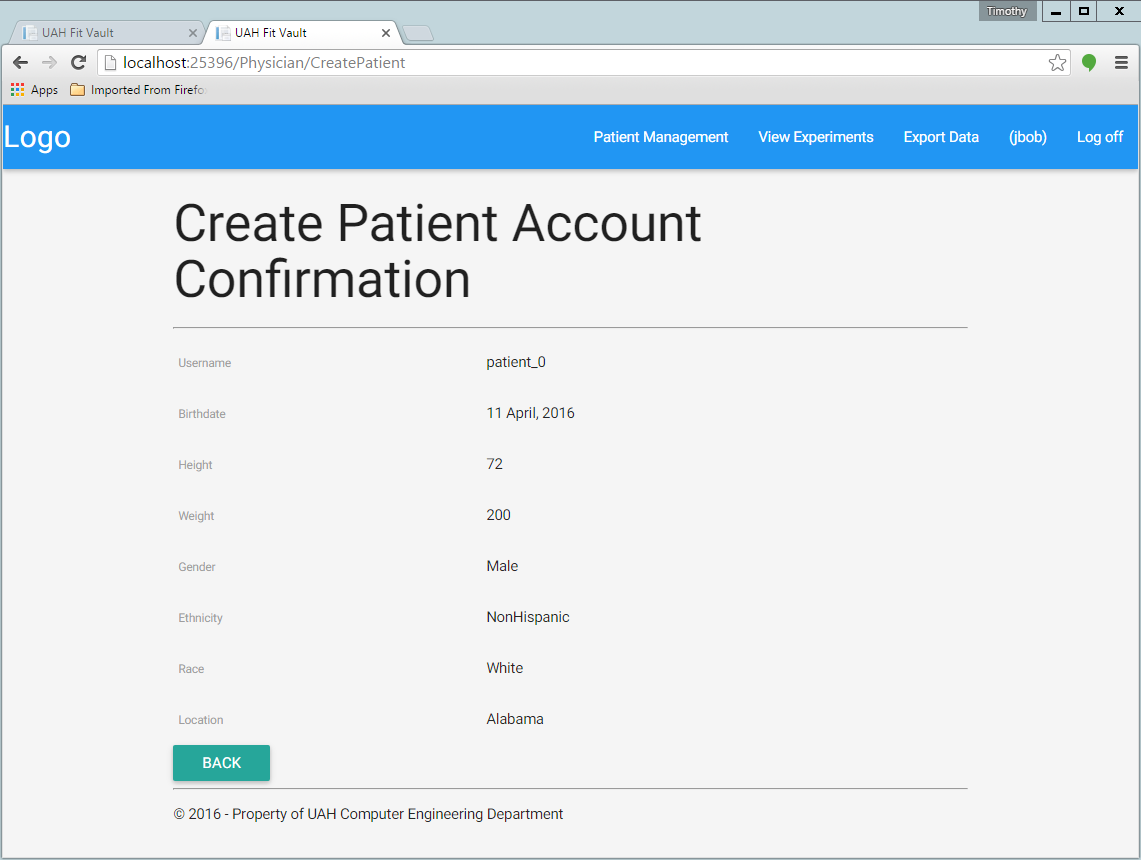
\includegraphics{create_patient_confirmation.png}


\paragraph{System Admin Account}
\label{user_guide/account_creation:system-admin-account}
UAHFitVault comes with a system administrator pre-configured. The username is `fitadmin' and the password is `Password1!'.
We recommend changing this after the installation before the server is made publicly available.

New System Admin accounts can be created by other System Admin accounts. From the System Admin account home page, click
the ``Create Admin'' button at the top right corner of the screen.

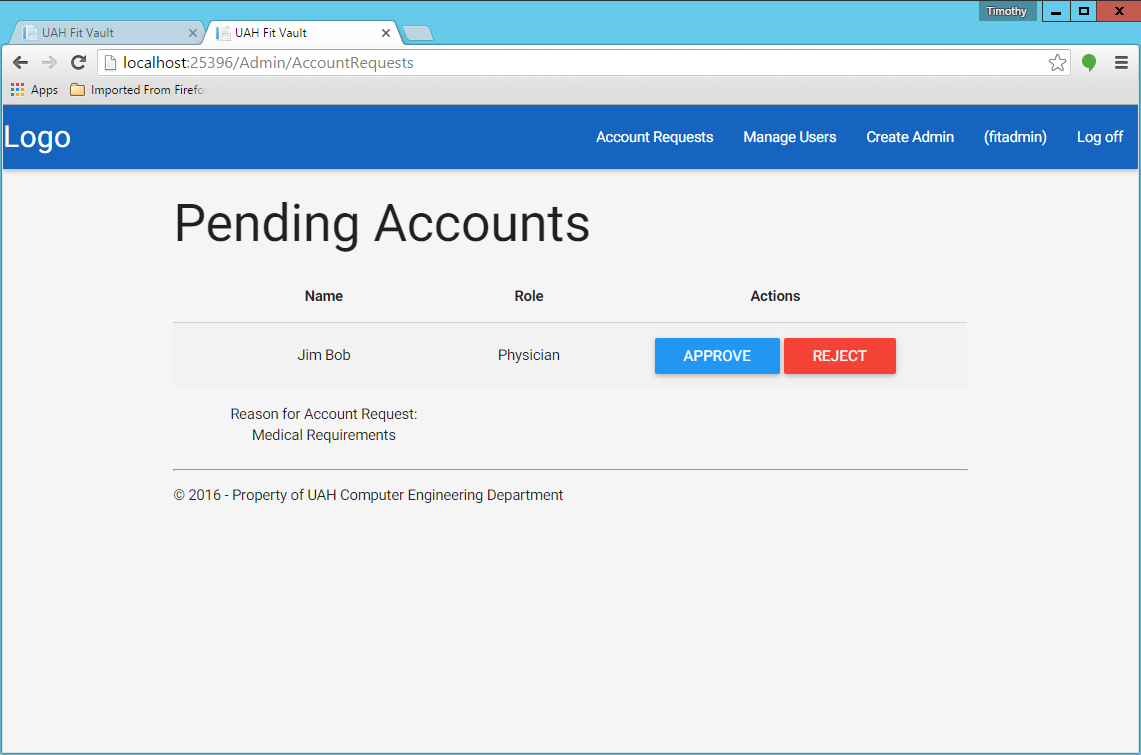
\includegraphics{account_approval.png}

You will be presented with a form to fill out for the system admin account information.

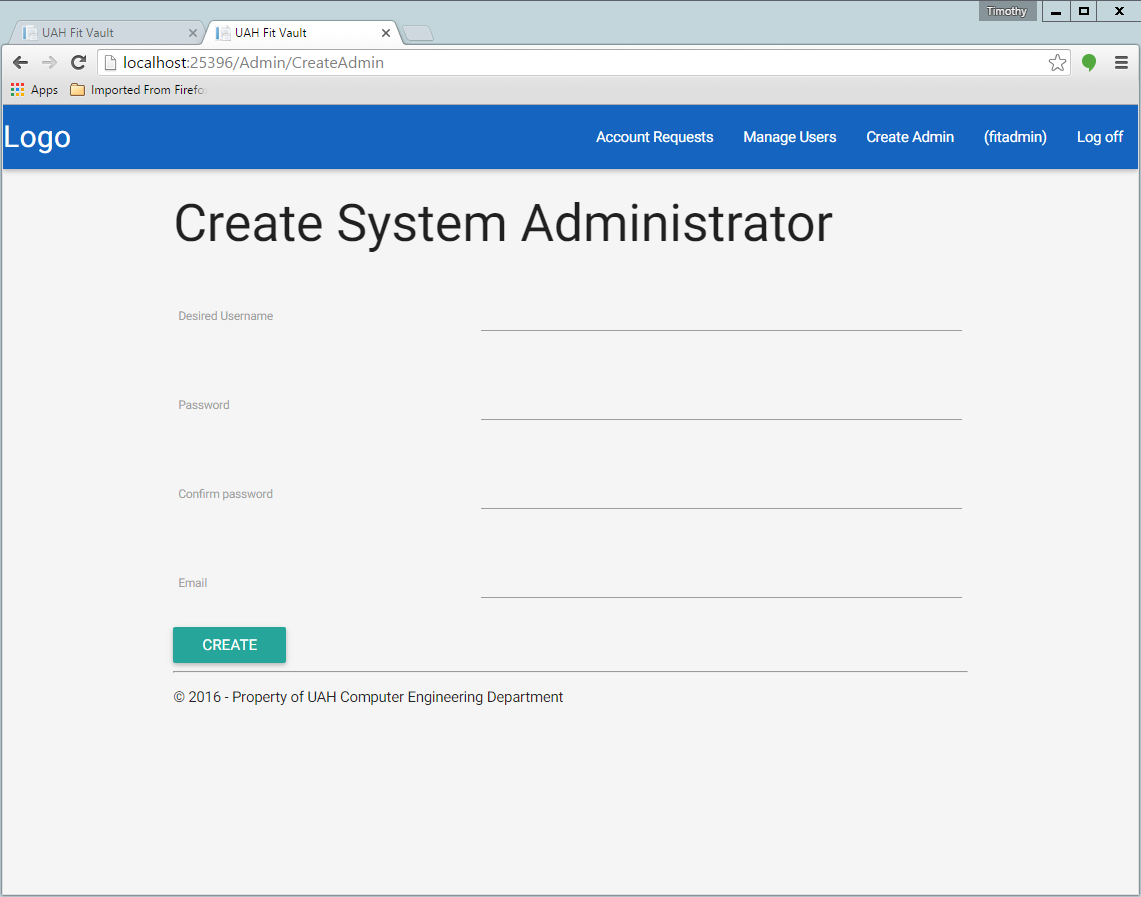
\includegraphics{create_admin.png}

Once the form is filled out and you click the create button, you should get a confirmation page.

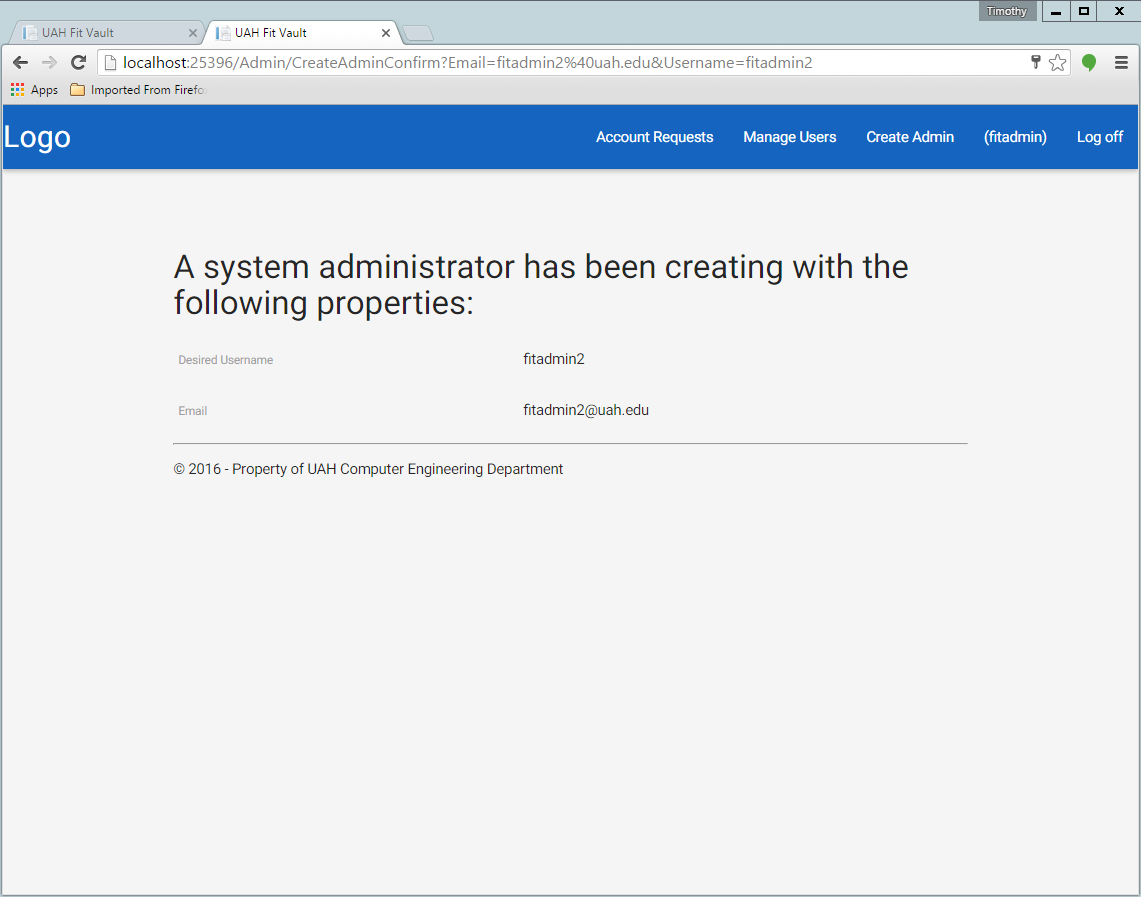
\includegraphics{create_admin_confirmation.png}


\subsubsection{Account Approval}
\label{user_guide/account_approval:id1}\label{user_guide/account_approval::doc}\label{user_guide/account_approval:account-approval}\setbox0\vbox{
\begin{minipage}{0.95\linewidth}
\textbf{Table of Contents}

\medskip

\begin{itemize}
\item {} 
{\hyperref[user_guide/account_approval:account-approval]{Account Approval}}

\end{itemize}
\end{minipage}}
\begin{center}\setlength{\fboxsep}{5pt}\shadowbox{\box0}\end{center}

There are 2 types of accounts that need approval:
\begin{itemize}
\item {} 
physician

\item {} 
experiment admin

\end{itemize}

To approve an account, login with your system administrator credentials. Then, click on the ``Account Requests''
button at the top right of the page. This should bring you to a page that looks like this:

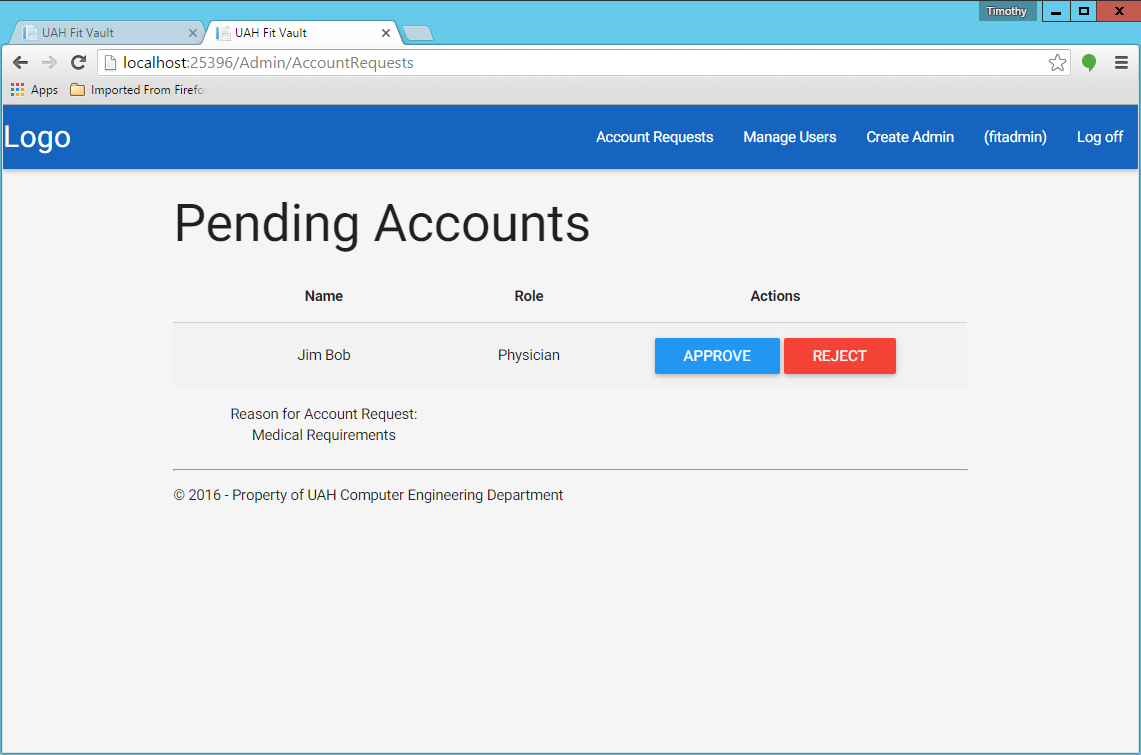
\includegraphics{account_approval.png}

You can then click on the ``APPROVE'' or ``REJECT'' button for the corresponding account you wish to approve or reject.


\subsubsection{Account Deletion}
\label{user_guide/account_deletion:account-deletion}\label{user_guide/account_deletion::doc}\label{user_guide/account_deletion:id1}\setbox0\vbox{
\begin{minipage}{0.95\linewidth}
\textbf{Table of Contents}

\medskip

\begin{itemize}
\item {} 
{\hyperref[user_guide/account_deletion:account-deletion]{Account Deletion}}

\end{itemize}
\end{minipage}}
\begin{center}\setlength{\fboxsep}{5pt}\shadowbox{\box0}\end{center}

Accounts can only be deleted by the System Administrator. Login as the system admin and click the ``Manage Users'' button
at the top right corner of the screen. You should be taken to a page like the one below:

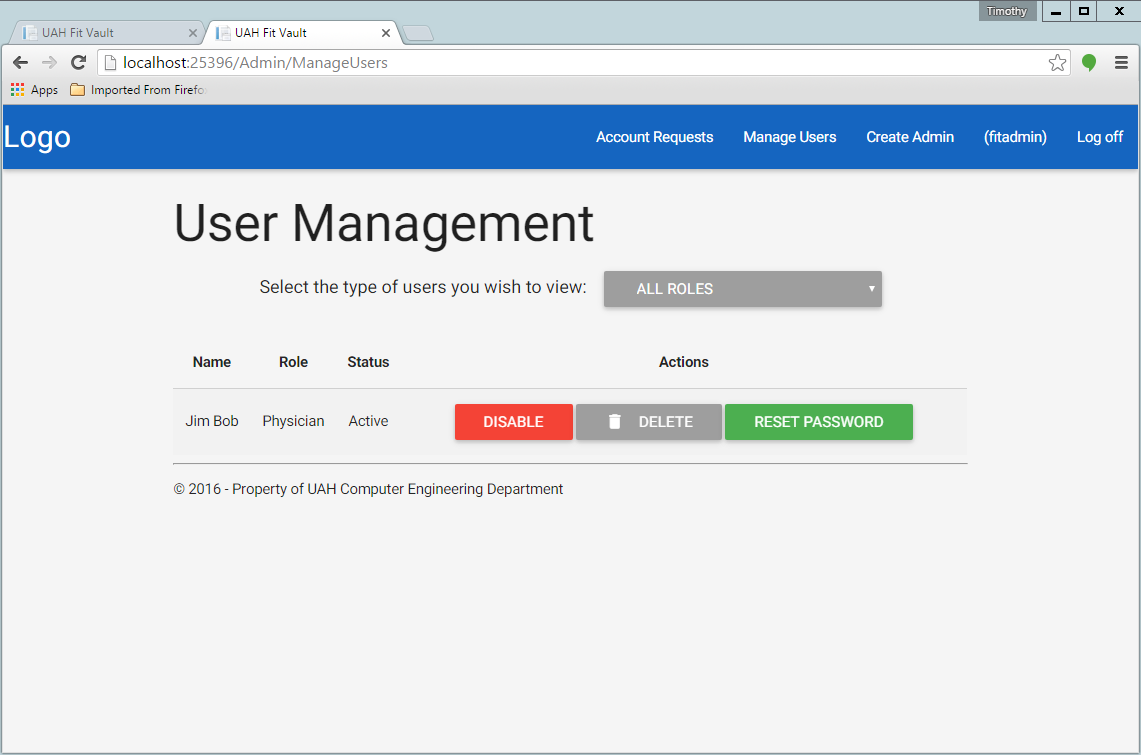
\includegraphics{manage_users.png}

From here you can use the roles filter to help you find the account to delete. Just click the ``Delete'' button that
corresponds to the account you wish to delete. If the delete worked the account should disappear from the list.


\subsubsection{Account Editing}
\label{user_guide/account_edit:account-edit}\label{user_guide/account_edit::doc}\label{user_guide/account_edit:account-editing}\setbox0\vbox{
\begin{minipage}{0.95\linewidth}
\textbf{Table of Contents}

\medskip

\begin{itemize}
\item {} 
{\hyperref[user_guide/account_edit:account-editing]{Account Editing}}
\begin{itemize}
\item {} 
{\hyperref[user_guide/account_edit:physician-account]{Physician Account}}

\item {} 
{\hyperref[user_guide/account_edit:experiment-admin-account]{Experiment Admin Account}}

\item {} 
{\hyperref[user_guide/account_edit:patient-account]{Patient Account}}
\begin{itemize}
\item {} 
{\hyperref[user_guide/account_edit:using-physician]{Using Physician}}

\item {} 
{\hyperref[user_guide/account_edit:using-patient]{Using Patient}}

\end{itemize}

\item {} 
{\hyperref[user_guide/account_edit:system-admin-account]{System Admin Account}}

\end{itemize}

\end{itemize}
\end{minipage}}
\begin{center}\setlength{\fboxsep}{5pt}\shadowbox{\box0}\end{center}

Users have the ability to edit their account information.


\paragraph{Physician Account}
\label{user_guide/account_edit:physician-account}\label{user_guide/account_edit:edit-physician-account}
To edit a physician account, you must be logged in as the physician. After login, click on the username at the top
right corner of the screen. You should be taken to a page like below:

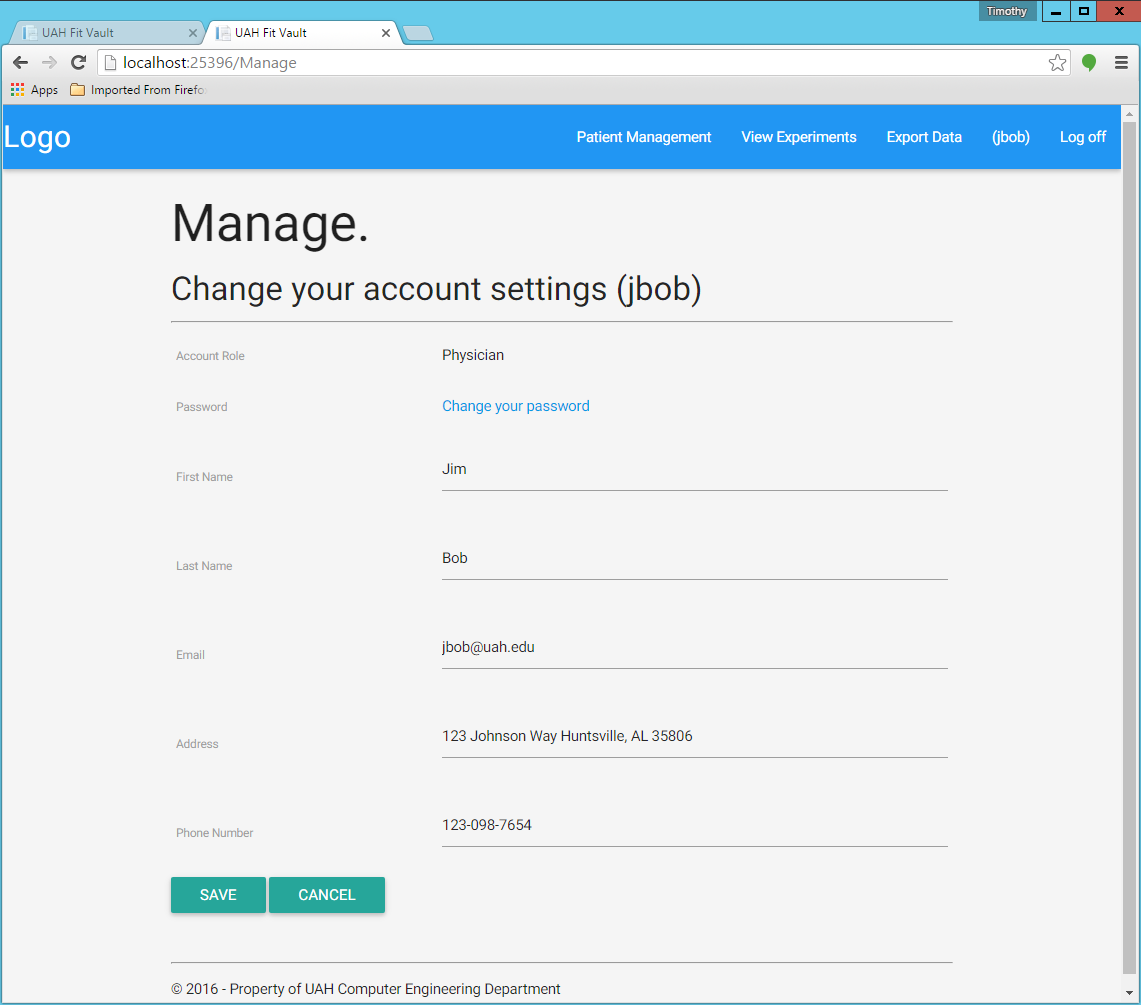
\includegraphics{account_management_physician.png}

After you edit the information you wish to edit, click the ``save'' button at the bottom. You should be taken to a confirmation
page like this:

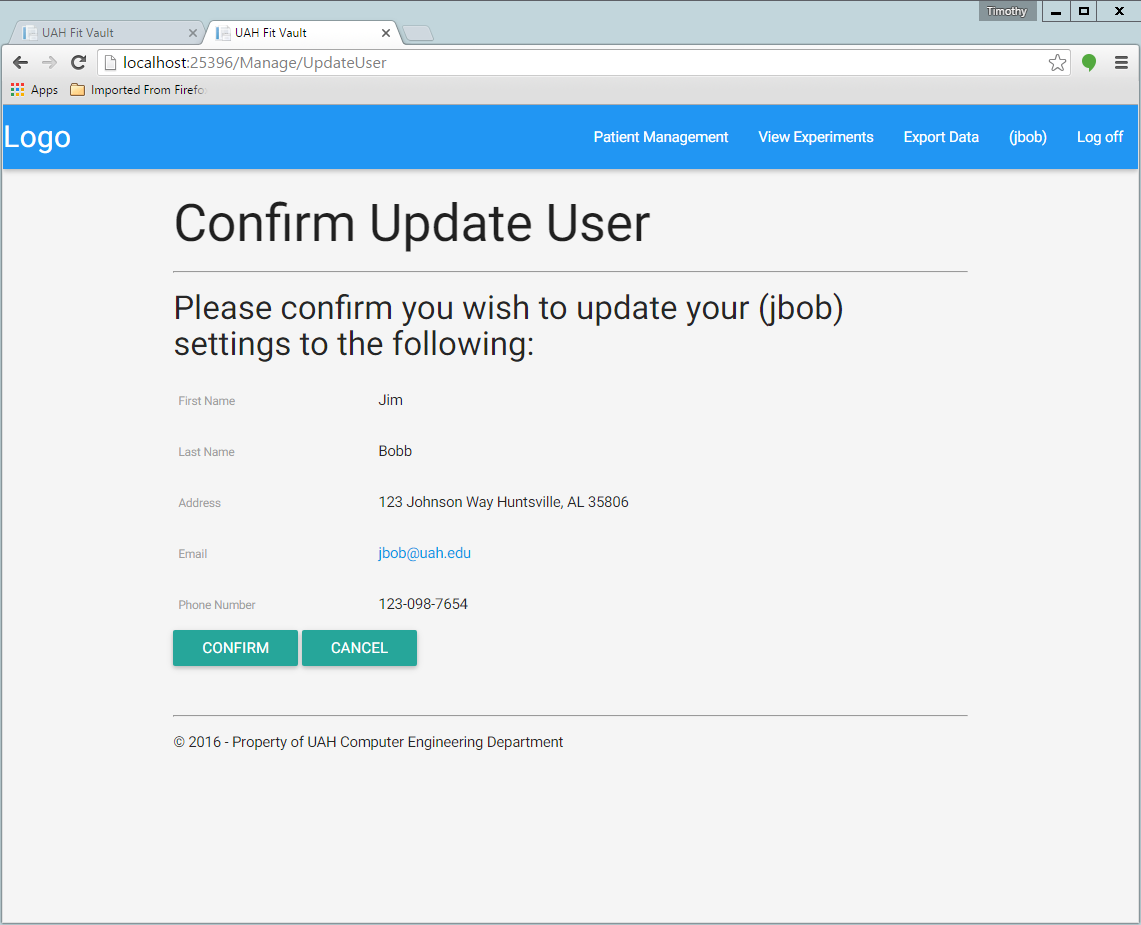
\includegraphics{account_management_physician_confirmation.png}

Click ``Confirm'' and you changes will be saved.


\paragraph{Experiment Admin Account}
\label{user_guide/account_edit:experiment-admin-account}
Editing an Experiment Admin account is exactly the same as editing a {\hyperref[user_guide/account_edit:edit-physician-account]{\emph{Physician}}} account.


\paragraph{Patient Account}
\label{user_guide/account_edit:patient-account}
Patient accounts can be edited by either the patient or the patient's physician.


\subparagraph{Using Physician}
\label{user_guide/account_edit:using-physician}
To edit it using a physician, login using the physician's credentials then click on the ``Patient Management'' button
at the top right corner of the page. You should then be taken to a page that looks like this:

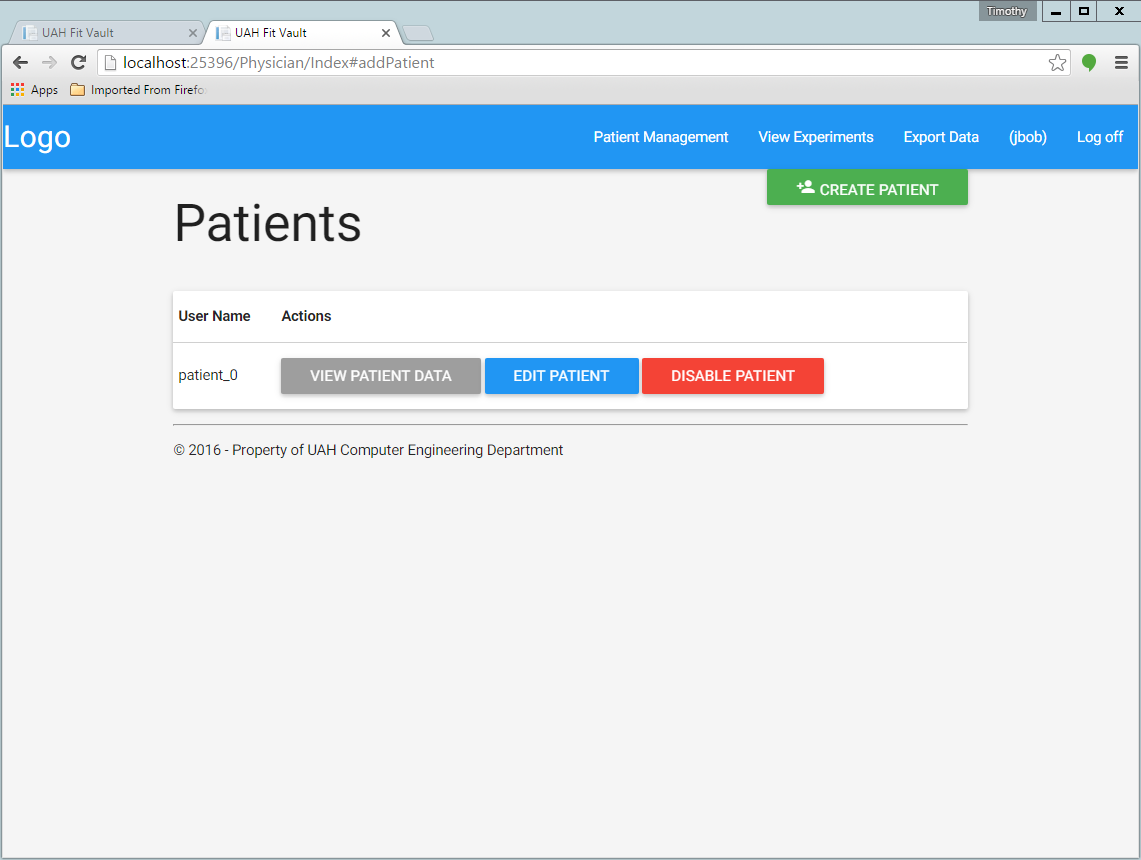
\includegraphics{patient_management.png}

Then click on the ``EDIT PATIENT'' button for the corresponding patient you want to edit. This will bring you to the
following page:

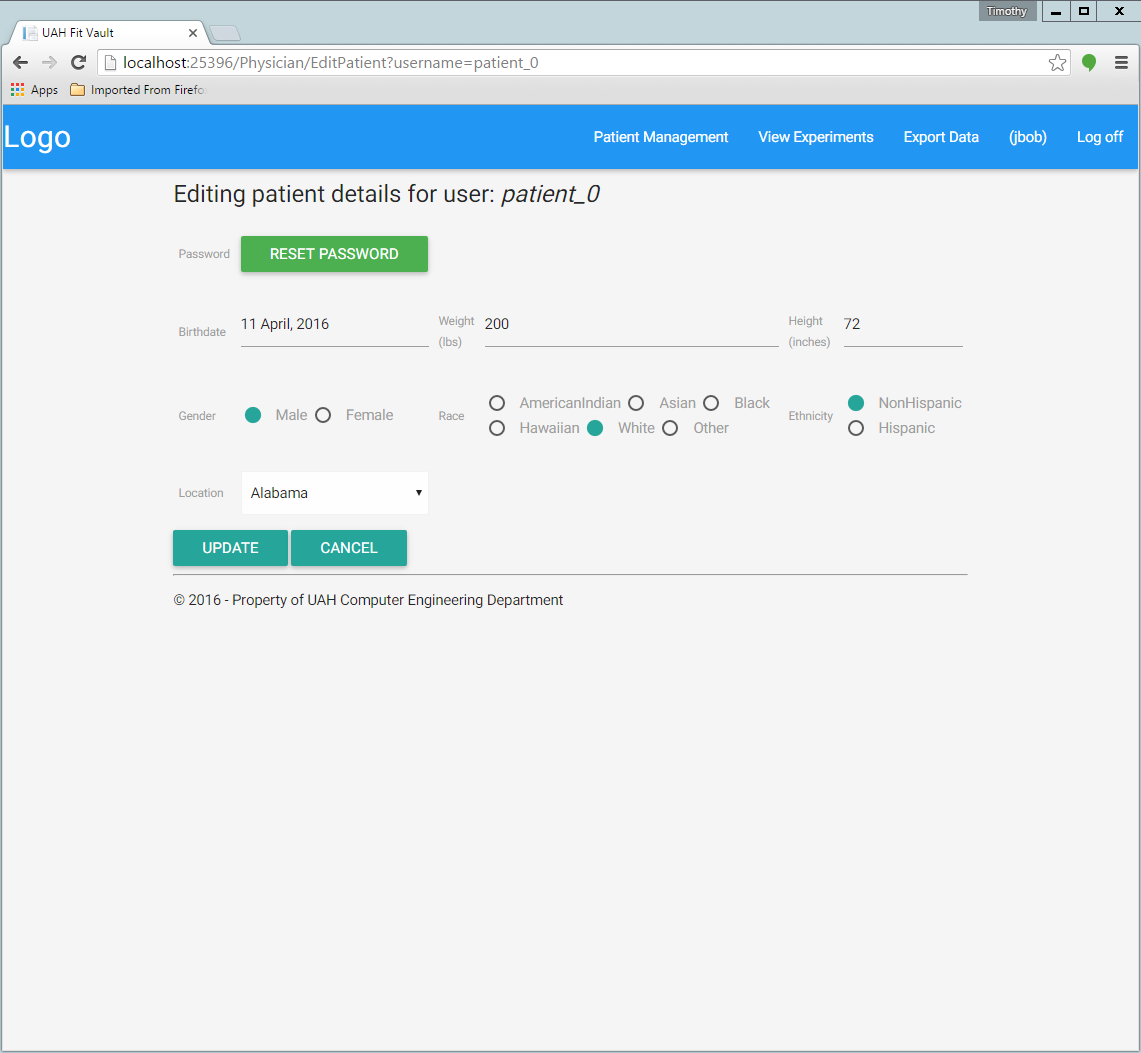
\includegraphics{edit_patient_account_physician.png}

Use the form to edit any of the information you want to change. Then click on the ``UPDATE'' button.


\subparagraph{Using Patient}
\label{user_guide/account_edit:using-patient}
To edit it using a patient, login using the patient's credentials then click on your patient user name at the top
right corner of the page. You should be brought to a page like this:

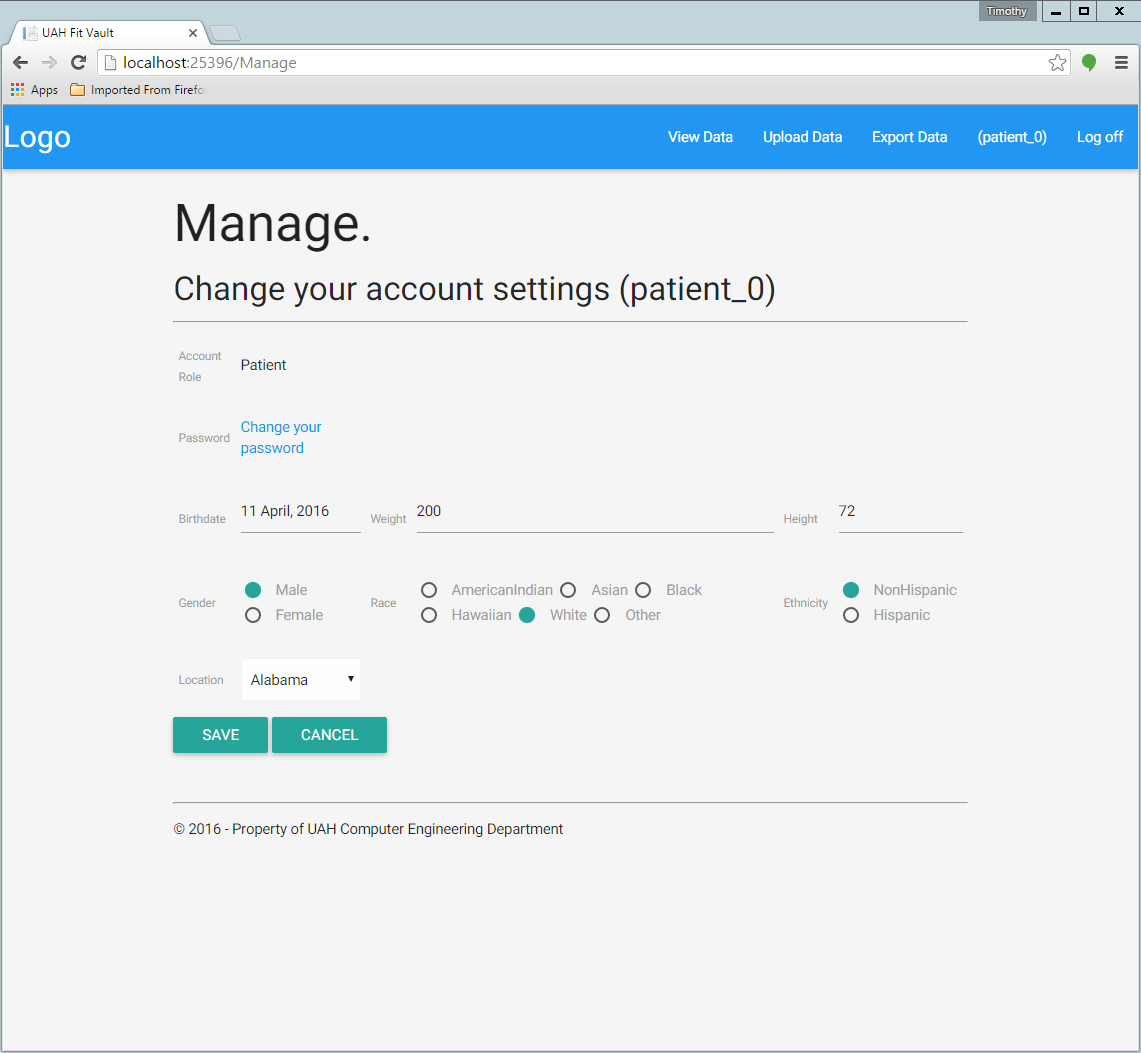
\includegraphics{edit_patient_account_patient.png}

Then fill out the form with any information you want to edit and click the ``SAVE'' button.


\paragraph{System Admin Account}
\label{user_guide/account_edit:system-admin-account}
To edit a System Admin account login as the system admin; then, click on the username at the top right corner of the
page. This should bring you to a page that looks like this:

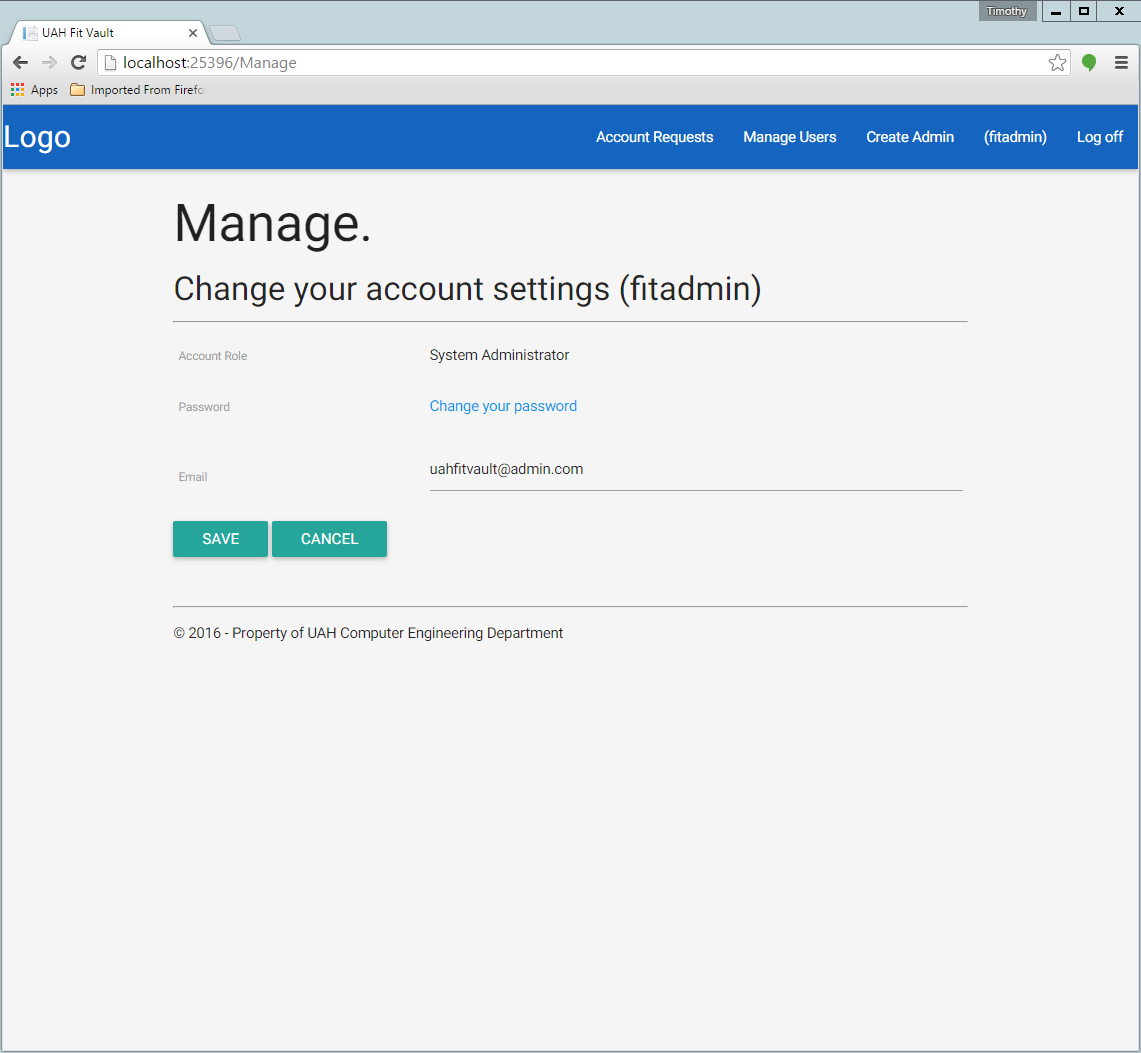
\includegraphics{edit_system_admin.png}

You can then use the form to edit any information you need for the system admin account. Then click the ``SAVE'' button
to save your changes.


\subsection{Experiment Management}
\label{user_guide/experiment_management::doc}\label{user_guide/experiment_management:experiment-management}\label{user_guide/experiment_management:id1}
Contents:


\subsubsection{Experiment Creation}
\label{user_guide/experiment_creation:experiment-creation}\label{user_guide/experiment_creation::doc}\label{user_guide/experiment_creation:id1}\setbox0\vbox{
\begin{minipage}{0.95\linewidth}
\textbf{Table of Contents}

\medskip

\begin{itemize}
\item {} 
{\hyperref[user_guide/experiment_creation:experiment-creation]{Experiment Creation}}

\end{itemize}
\end{minipage}}
\begin{center}\setlength{\fboxsep}{5pt}\shadowbox{\box0}\end{center}

Experiments can be created by an Experiment Admin. To create an experiment go to the home page and login with your
experiment admin credentials. Click on the ``Create Experiment'' button at the top right of the screen. This should
take you to a page like this:

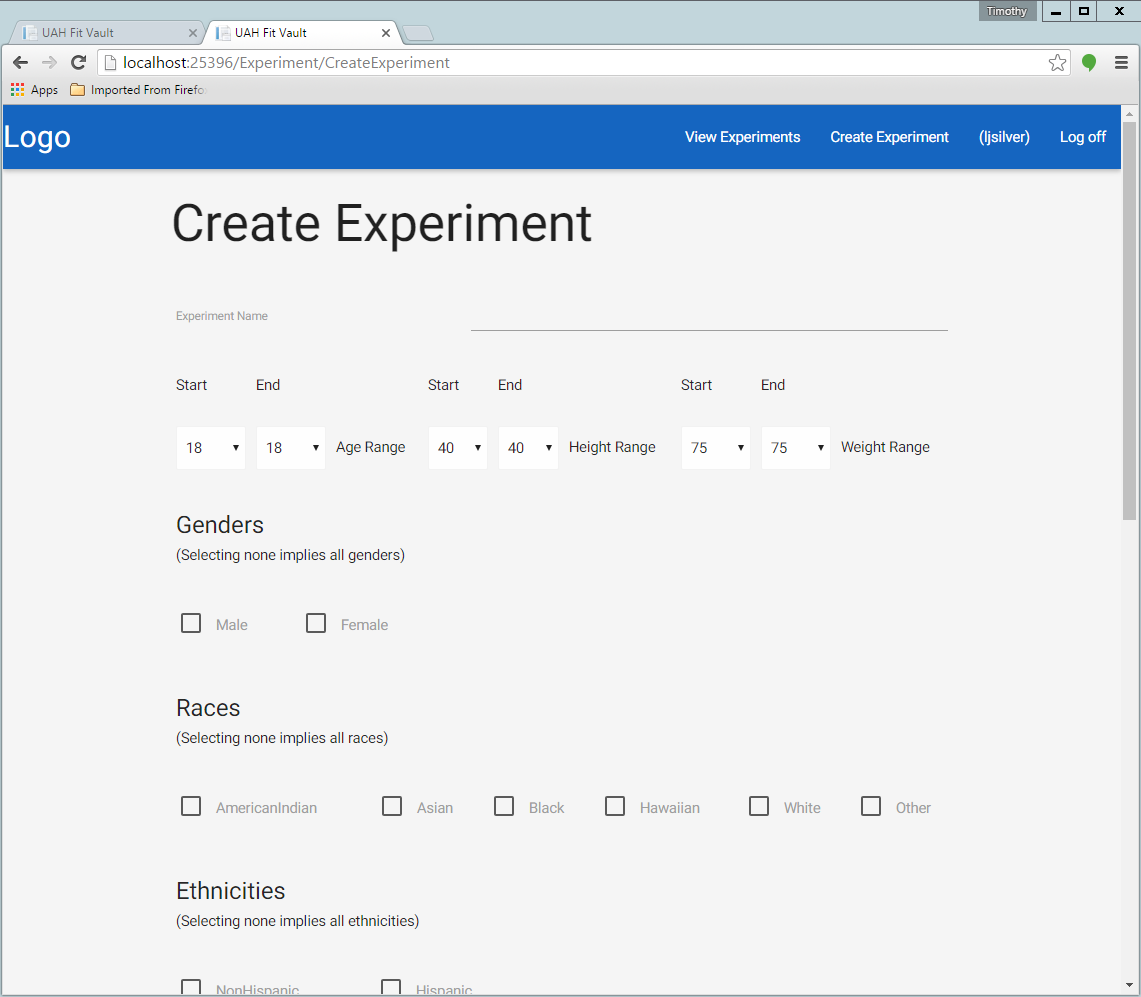
\includegraphics{create_experiment_1.png}

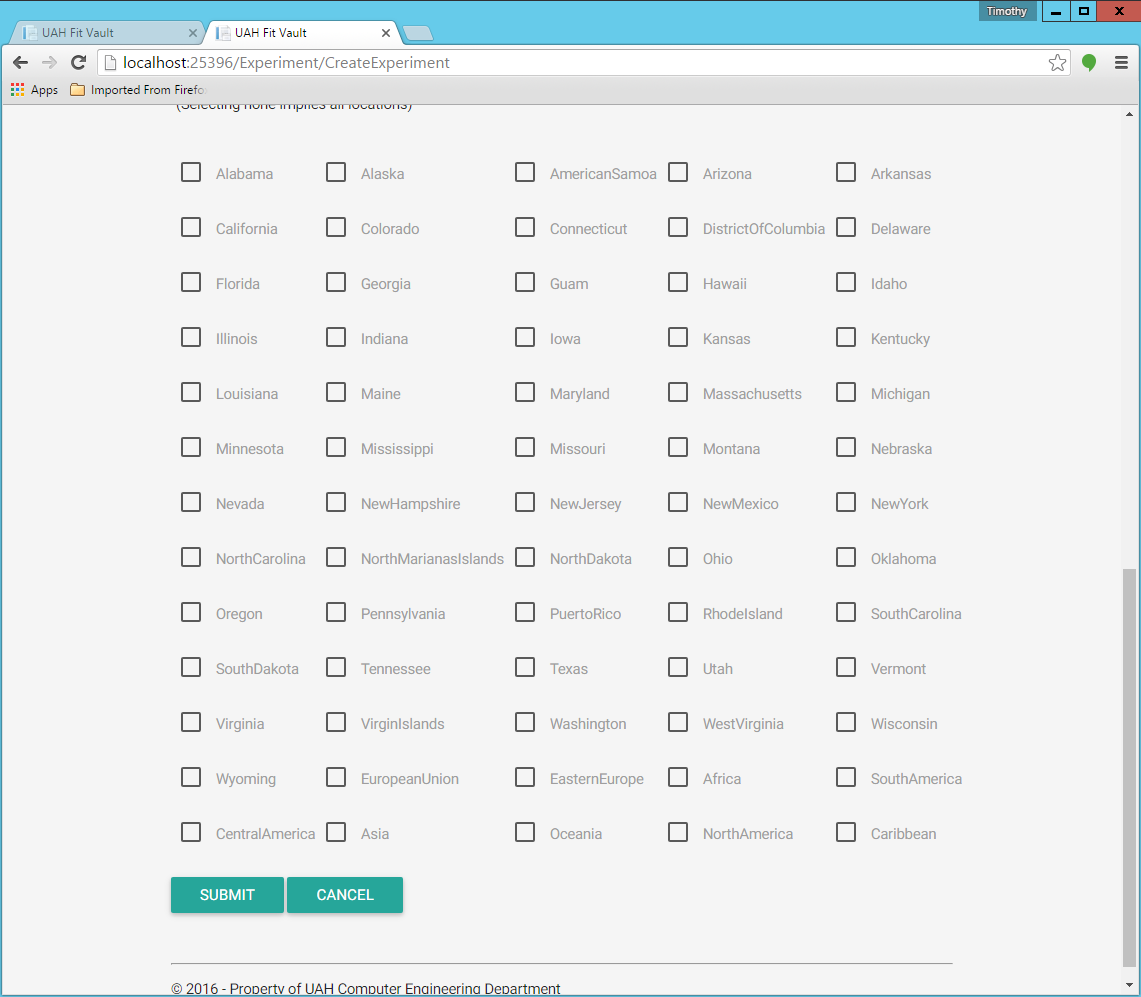
\includegraphics{create_experiment_2.png}

You can then fill out information that will filter out patients for your experiment. Once you have filled out the
form completely to your liking, click the ``SUBMIT'' button at the bottom of the form. If everything worked right, you
should be presented with a confirmation page like this:

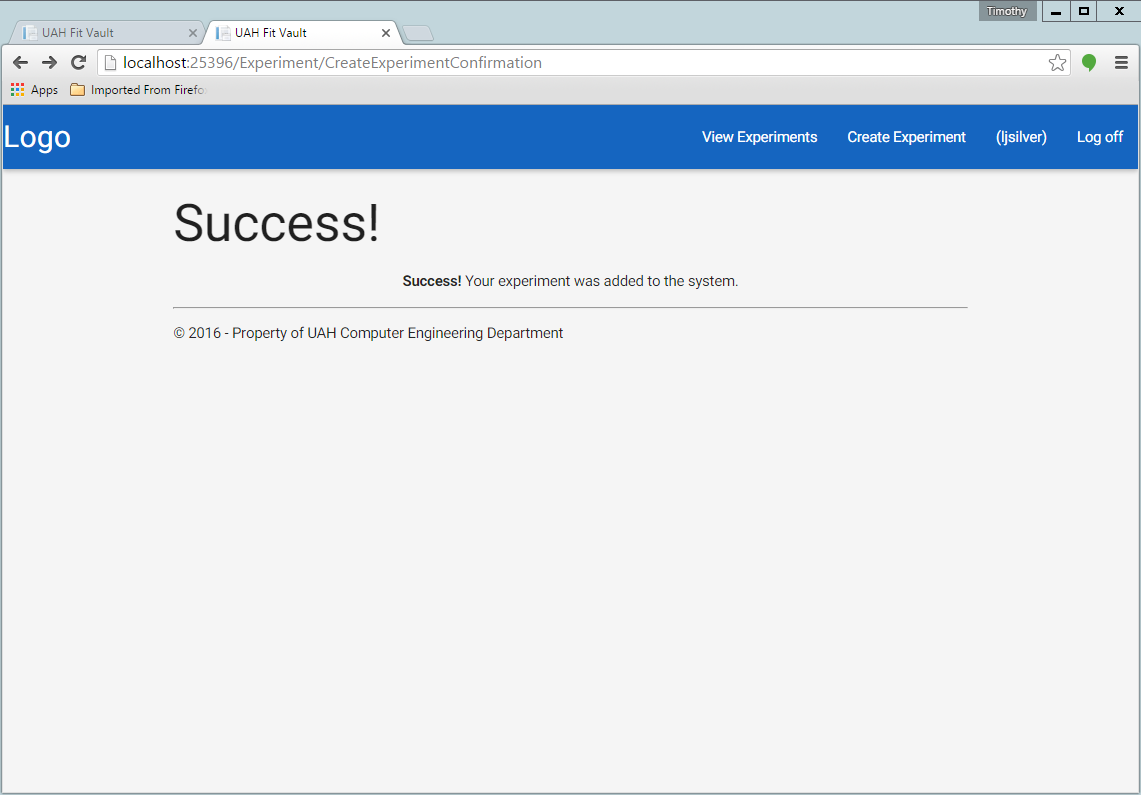
\includegraphics{create_experiment_confirmation.png}


\subsubsection{Experiment View}
\label{user_guide/experiment_view::doc}\label{user_guide/experiment_view:experiment-view}\label{user_guide/experiment_view:id1}\setbox0\vbox{
\begin{minipage}{0.95\linewidth}
\textbf{Table of Contents}

\medskip

\begin{itemize}
\item {} 
{\hyperref[user_guide/experiment_view:experiment-view]{Experiment View}}
\begin{itemize}
\item {} 
{\hyperref[user_guide/experiment_view:experiment-admin]{Experiment Admin}}

\item {} 
{\hyperref[user_guide/experiment_view:physicians]{Physicians}}

\end{itemize}

\end{itemize}
\end{minipage}}
\begin{center}\setlength{\fboxsep}{5pt}\shadowbox{\box0}\end{center}

Both Physicians and Experiment Admins can view experiments.


\paragraph{Experiment Admin}
\label{user_guide/experiment_view:experiment-admin}
Once an experiment has been created, login with your experiment admin credentials and click on the ``View Experiment'' button
at the top right corner of the page. You should be taken to a page that looks like this:

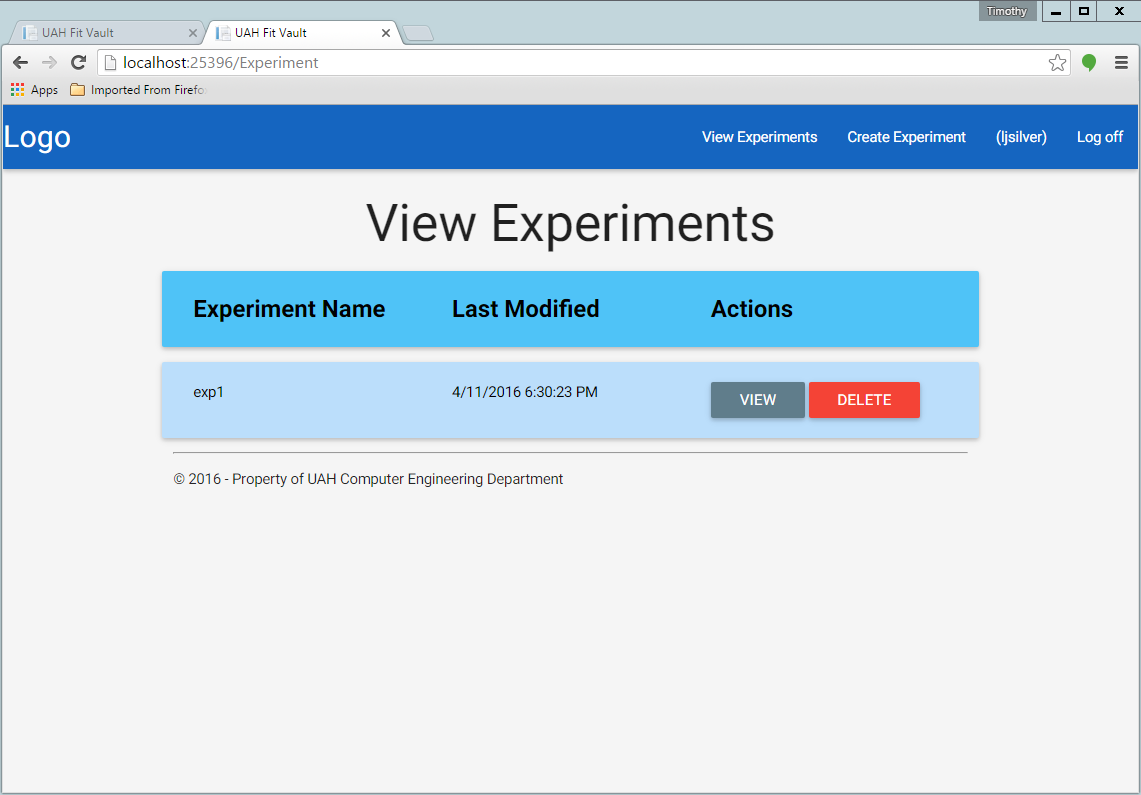
\includegraphics{view_experiments.png}

You can then click on the ``VIEW'' button of the corresponding experiment you want to view. Then this should take you
to to a page that looks like this:

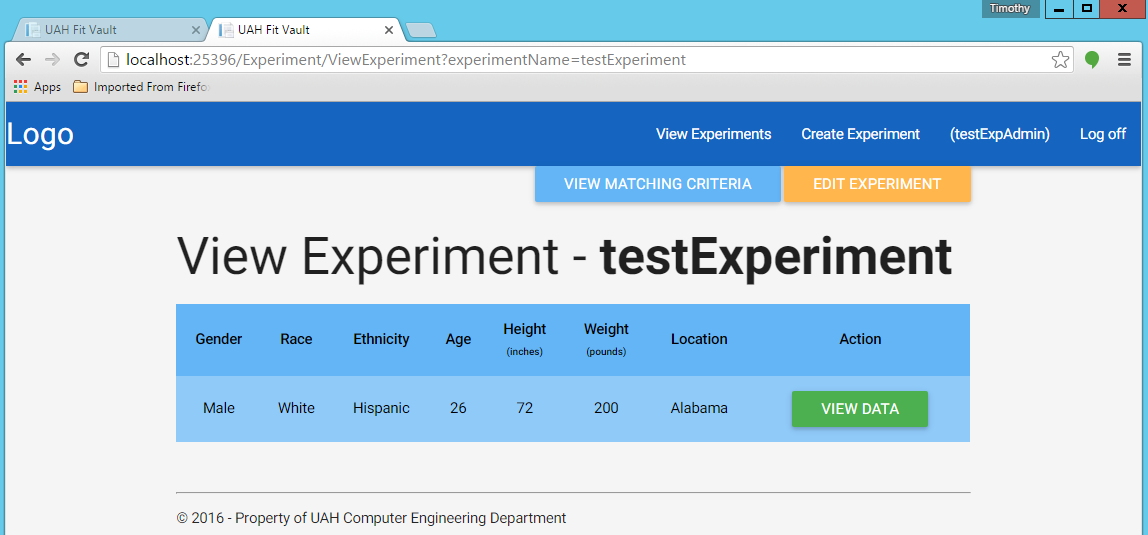
\includegraphics{view_experiments_expadmin.png}

You can now view the data for all the patients that fit into the experiment:

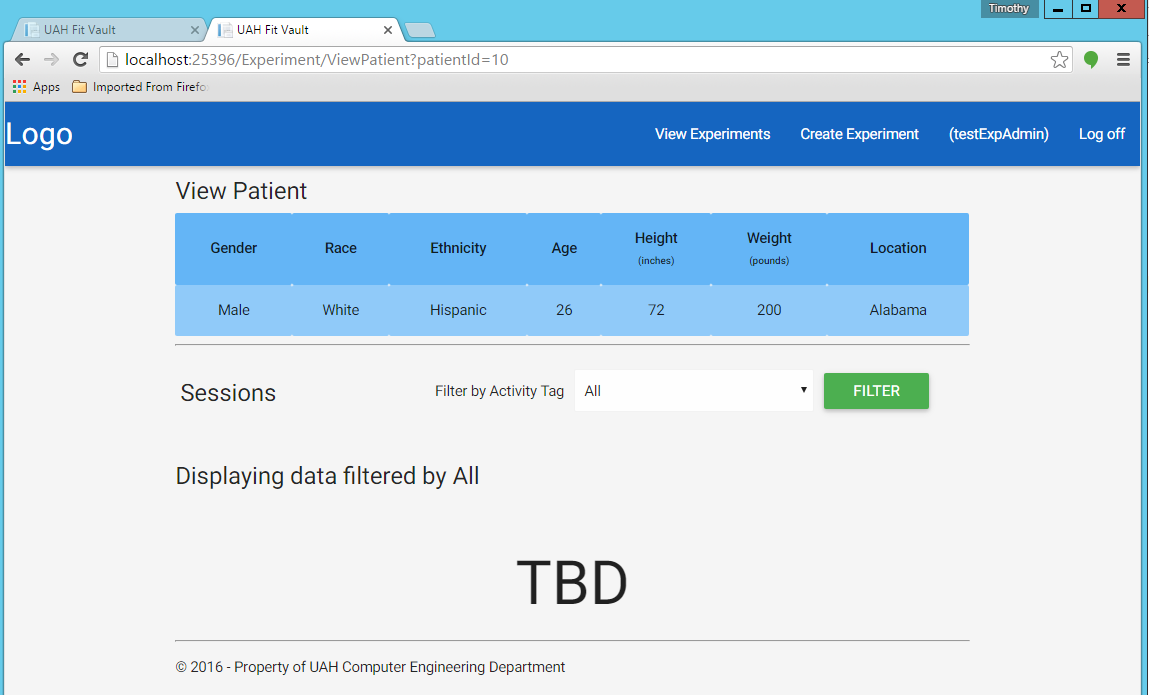
\includegraphics{view_experiments_expadmin_2.png}


\paragraph{Physicians}
\label{user_guide/experiment_view:physicians}
Login with your physician credentials and click the ``View Experiments'' button at the top right corner of the page.
You should be taken to a page that looks like this:

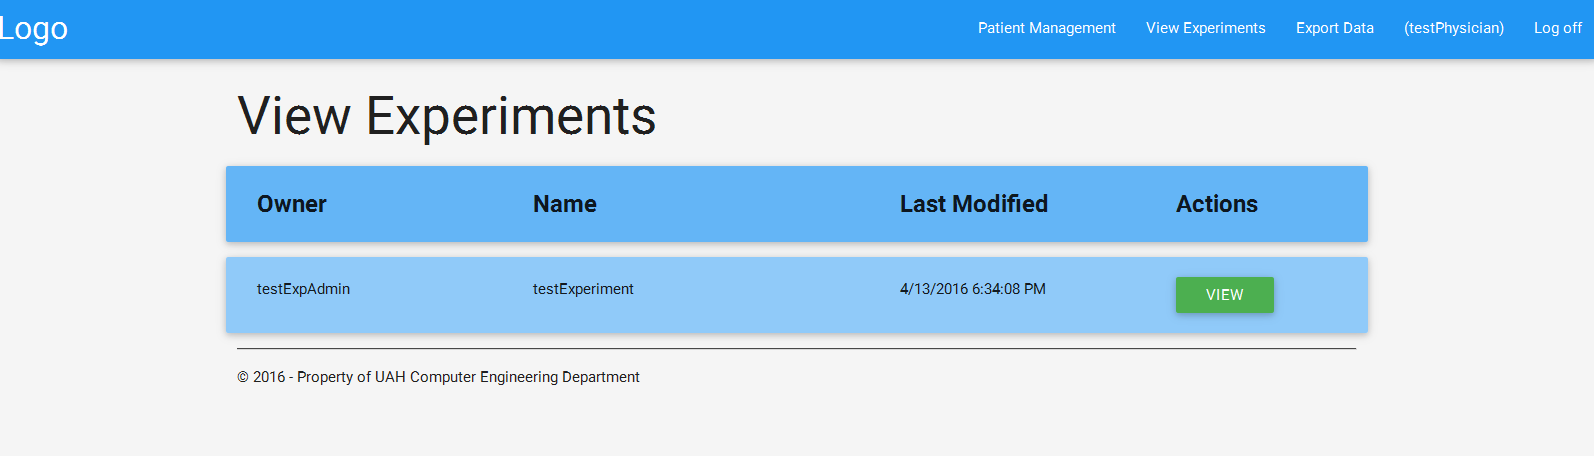
\includegraphics{view_experiments_physician.png}

You can then click on the green ``VIEW'' button to the corresponding experiment you want to view. This should take you
to a page that looks like this:

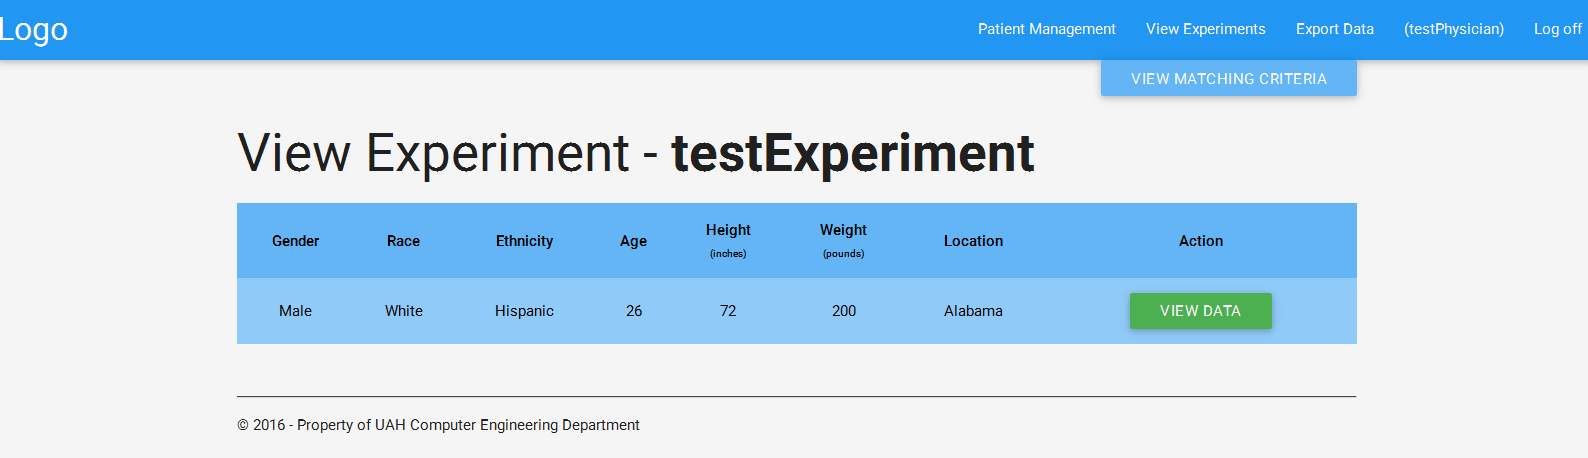
\includegraphics{view_experiments_physician_2.png}

You can now view the data for all the patients that fit into the experiment:

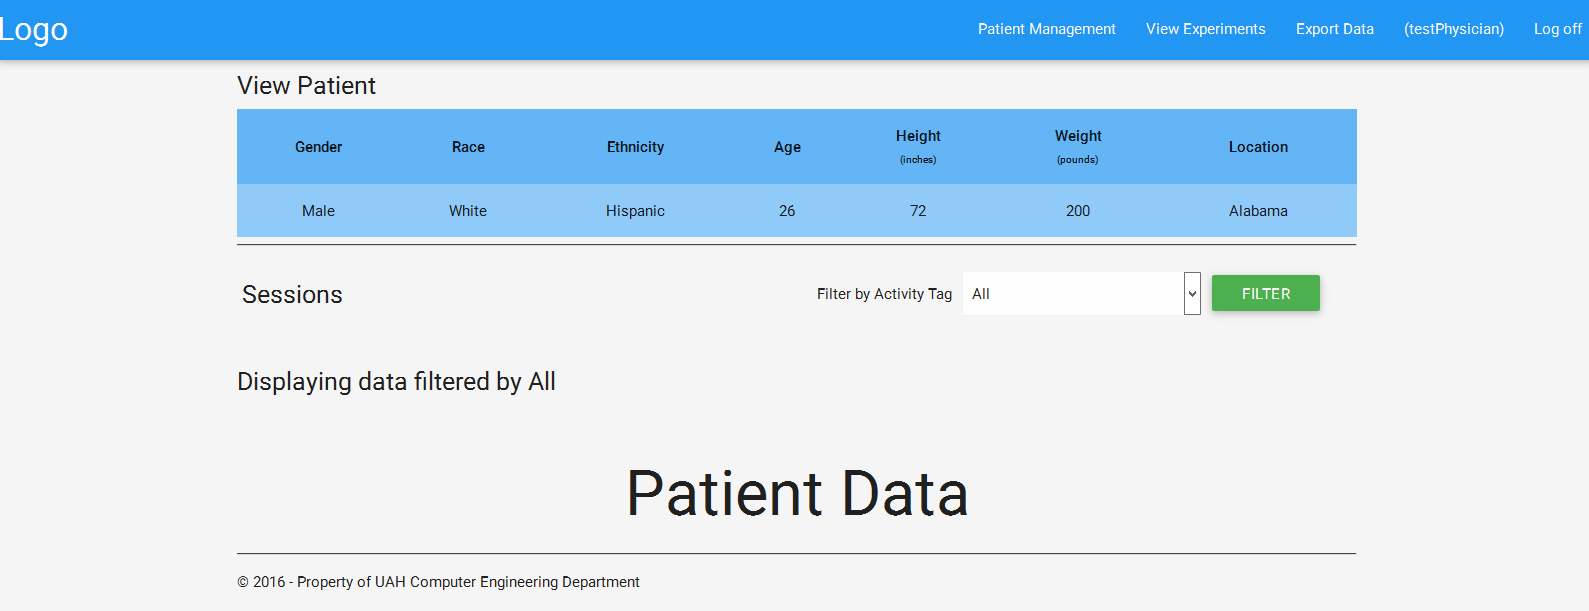
\includegraphics{view_experiments_physician_3.png}


\subsubsection{Experiment Deletion}
\label{user_guide/experiment_deletion:id1}\label{user_guide/experiment_deletion::doc}\label{user_guide/experiment_deletion:experiment-deletion}\setbox0\vbox{
\begin{minipage}{0.95\linewidth}
\textbf{Table of Contents}

\medskip

\begin{itemize}
\item {} 
{\hyperref[user_guide/experiment_deletion:experiment-deletion]{Experiment Deletion}}

\end{itemize}
\end{minipage}}
\begin{center}\setlength{\fboxsep}{5pt}\shadowbox{\box0}\end{center}

Only an Experiment Admin can delete experiments. To do this, simply login with your Experiment Admin credentials, and
click on the ``View Experiments'' button at the top right corner of the page. This should take you to a page that
looks like this:

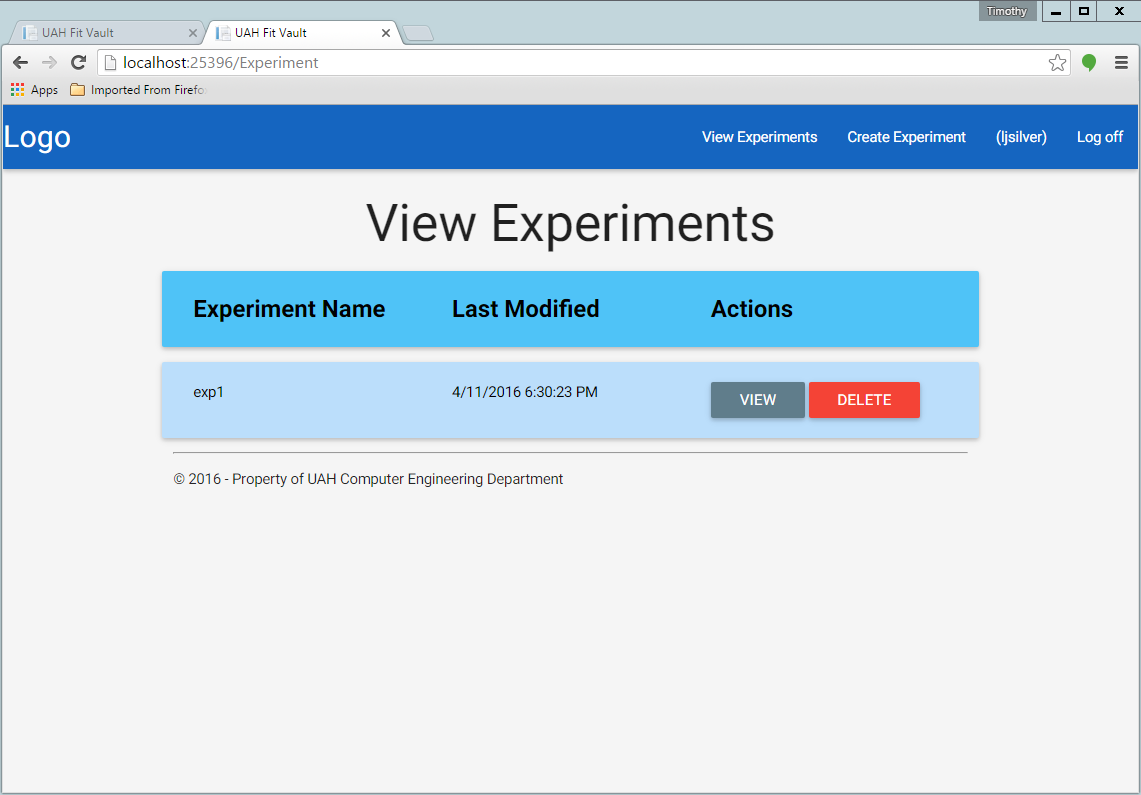
\includegraphics{view_experiments.png}

You can then click on the ``DELETE'' button of the corresponding experiment you want to delete.


\subsubsection{Experiment Exportation}
\label{user_guide/experiment_exportation:experiment-exportation}\label{user_guide/experiment_exportation::doc}\label{user_guide/experiment_exportation:id1}\setbox0\vbox{
\begin{minipage}{0.95\linewidth}
\textbf{Table of Contents}

\medskip

\begin{itemize}
\item {} 
{\hyperref[user_guide/experiment_exportation:experiment-exportation]{Experiment Exportation}}

\end{itemize}
\end{minipage}}
\begin{center}\setlength{\fboxsep}{5pt}\shadowbox{\box0}\end{center}

An Experiment Admin can export experiment data. Login as an experiment administrator. Then click on the ``View Experiment''
button.

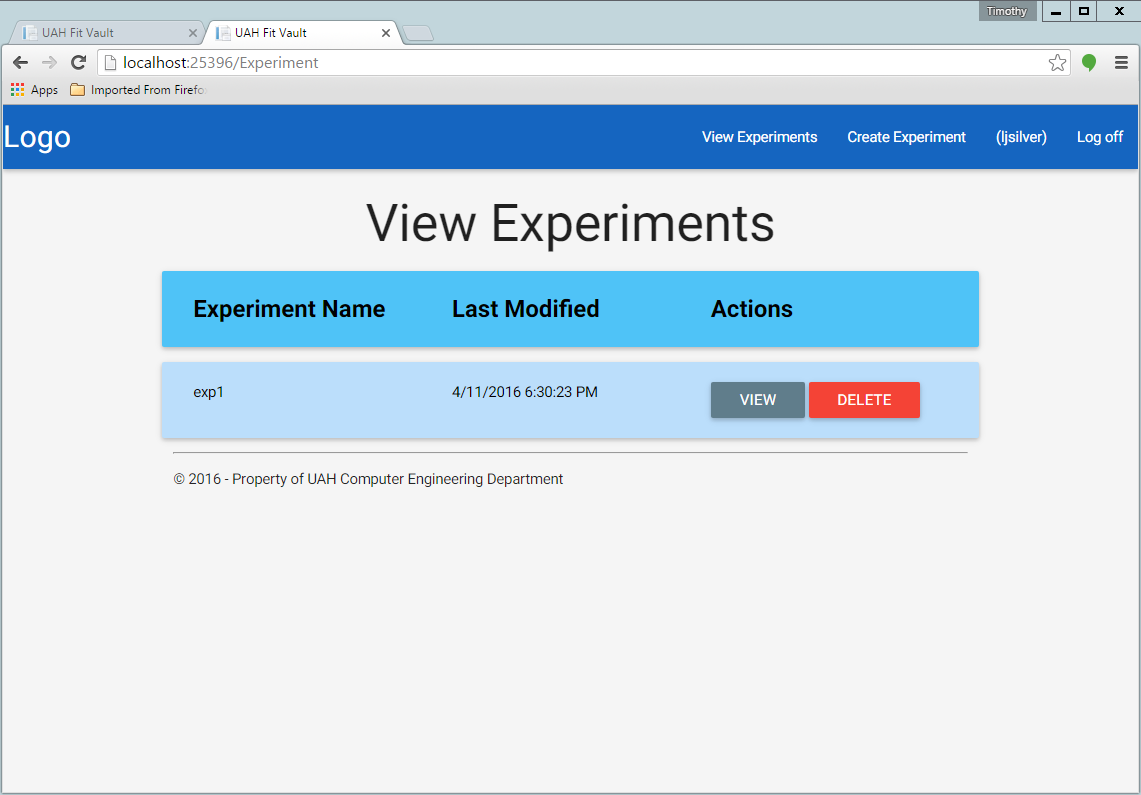
\includegraphics{view_experiments.png}

You should then see existing experiments. Click on the ``View'' button for the experiment you want to export. You should
see the following page:

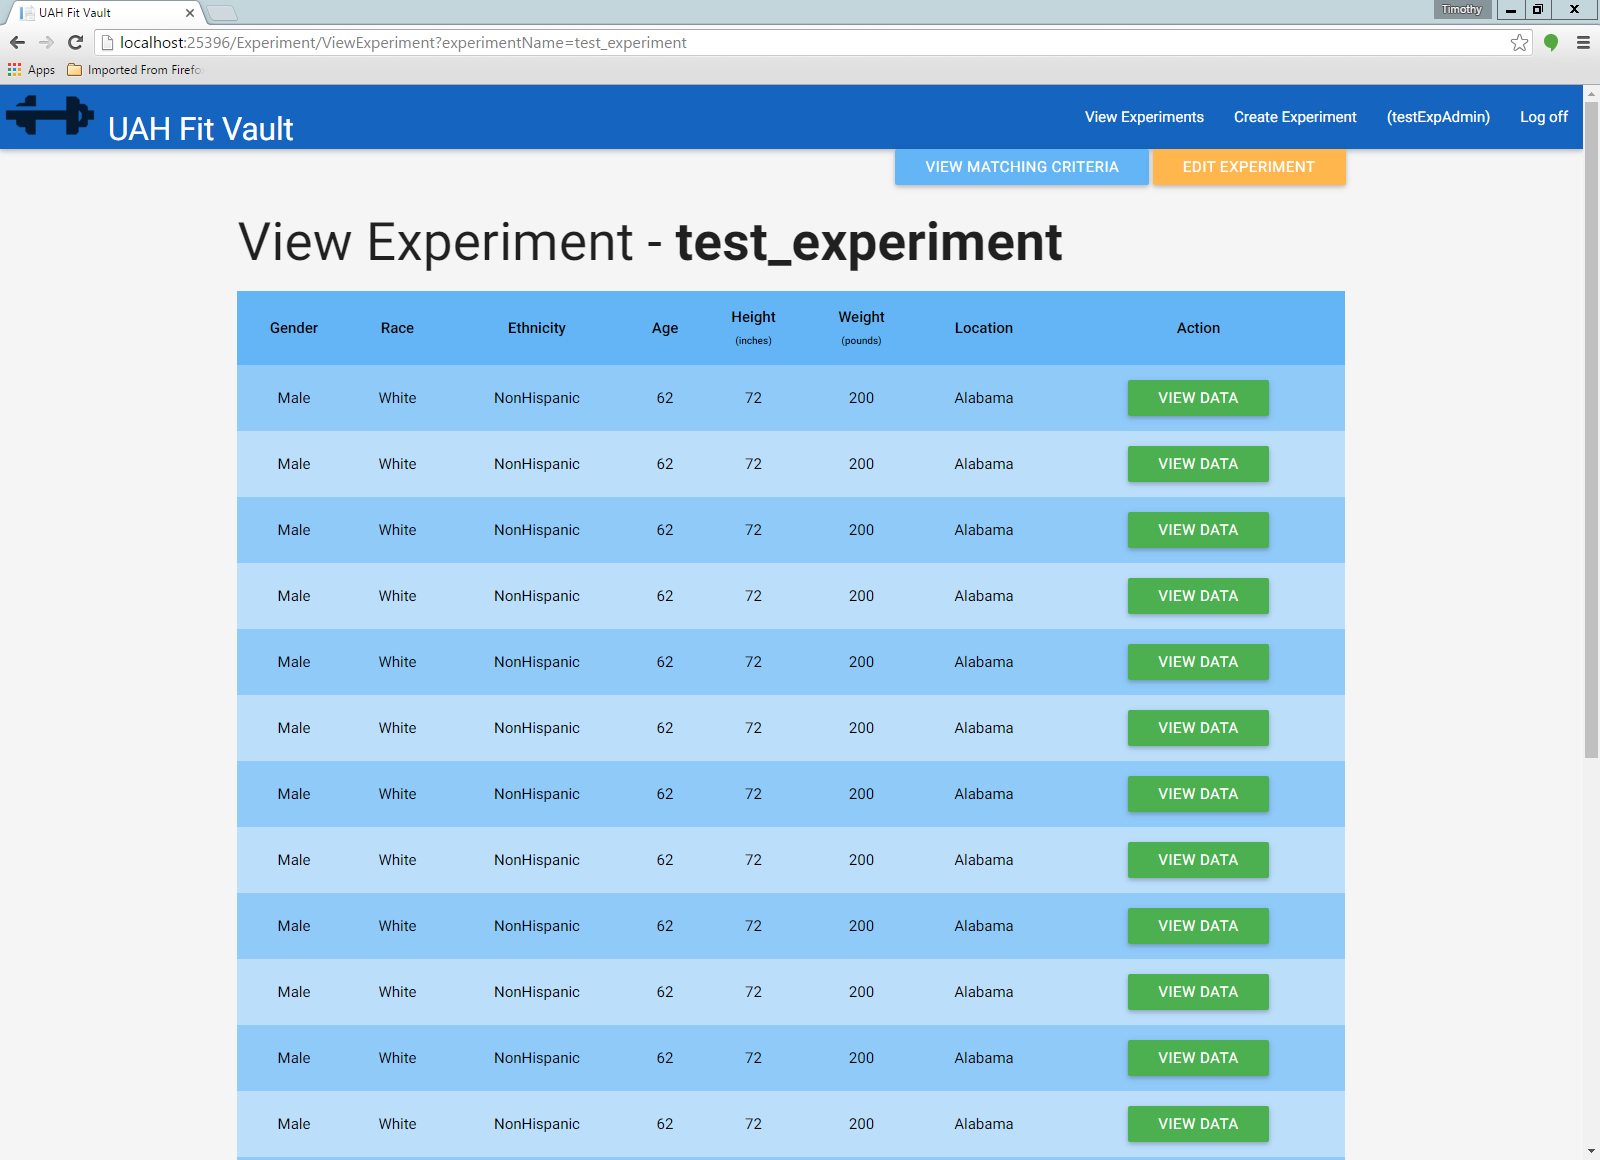
\includegraphics{view_experiments_expadmin_export.png}

Next click on the ``View Data'' button for the account you want to download data from. You should see a page that looks
like this:

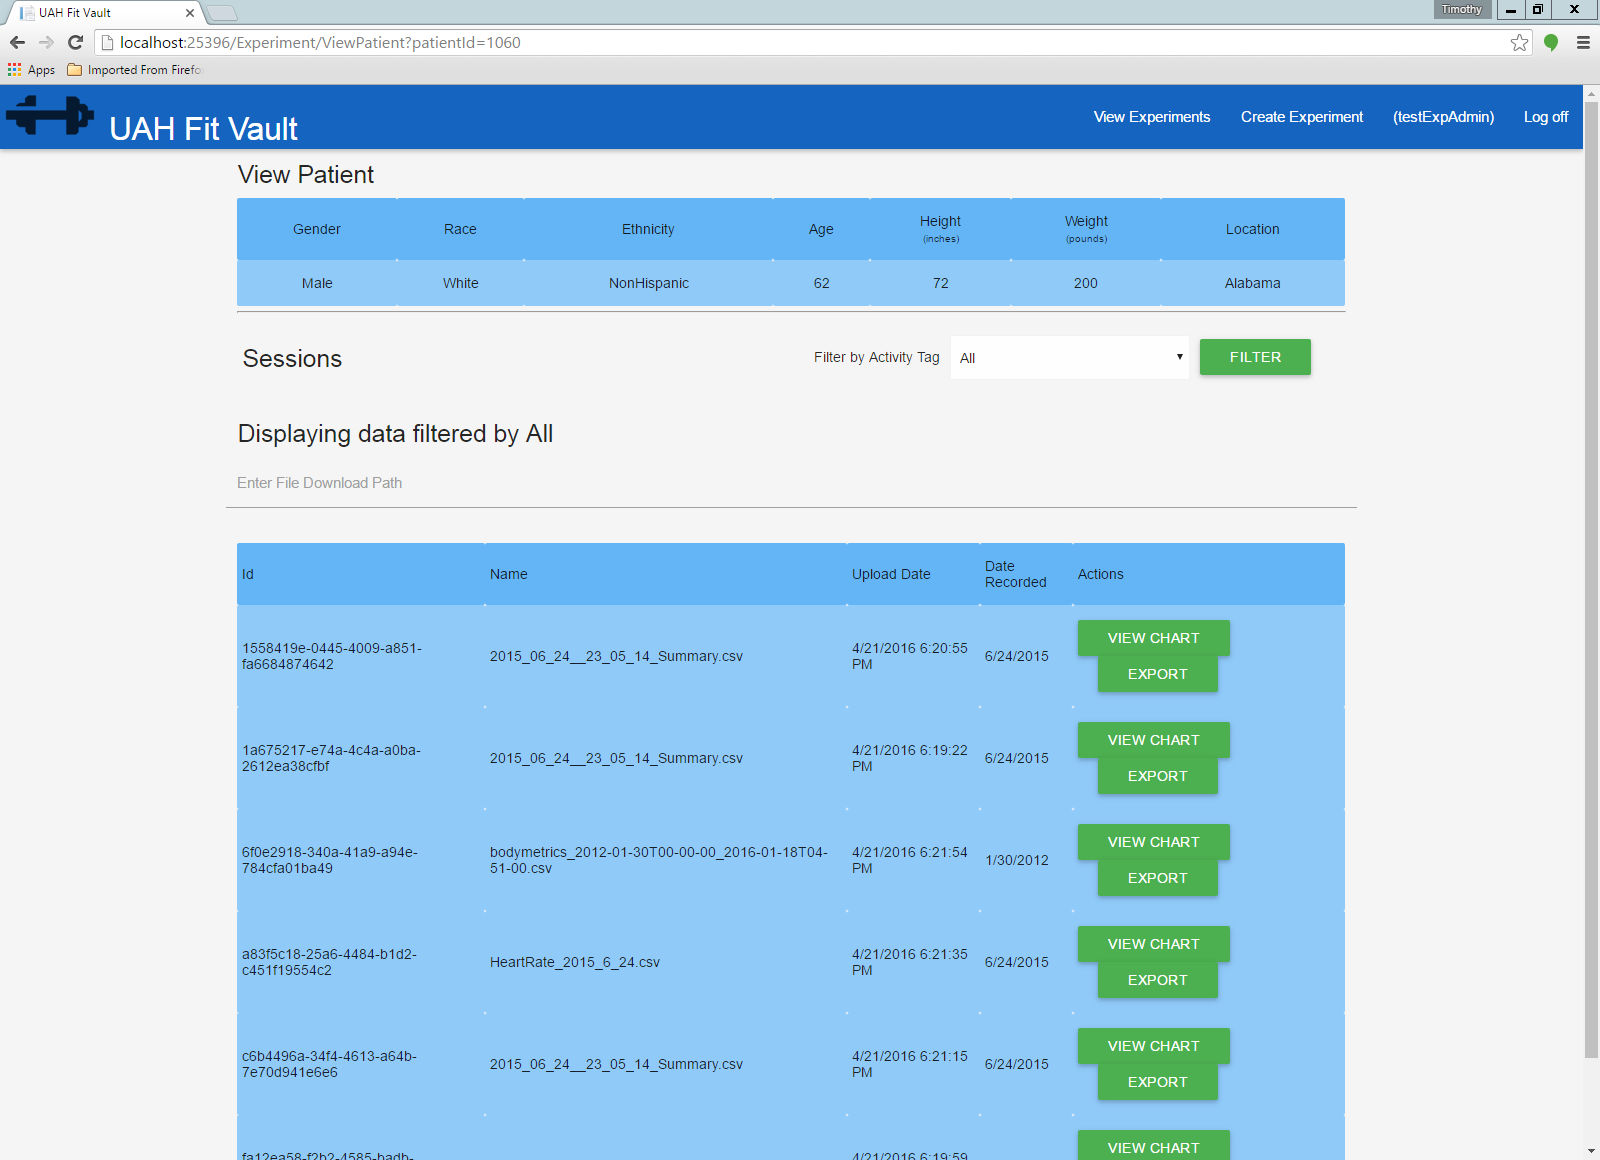
\includegraphics{view_experiments_expadmin_export_2.png}

You can then fill out the path and click on the ``Export'' button for the file you want to export.

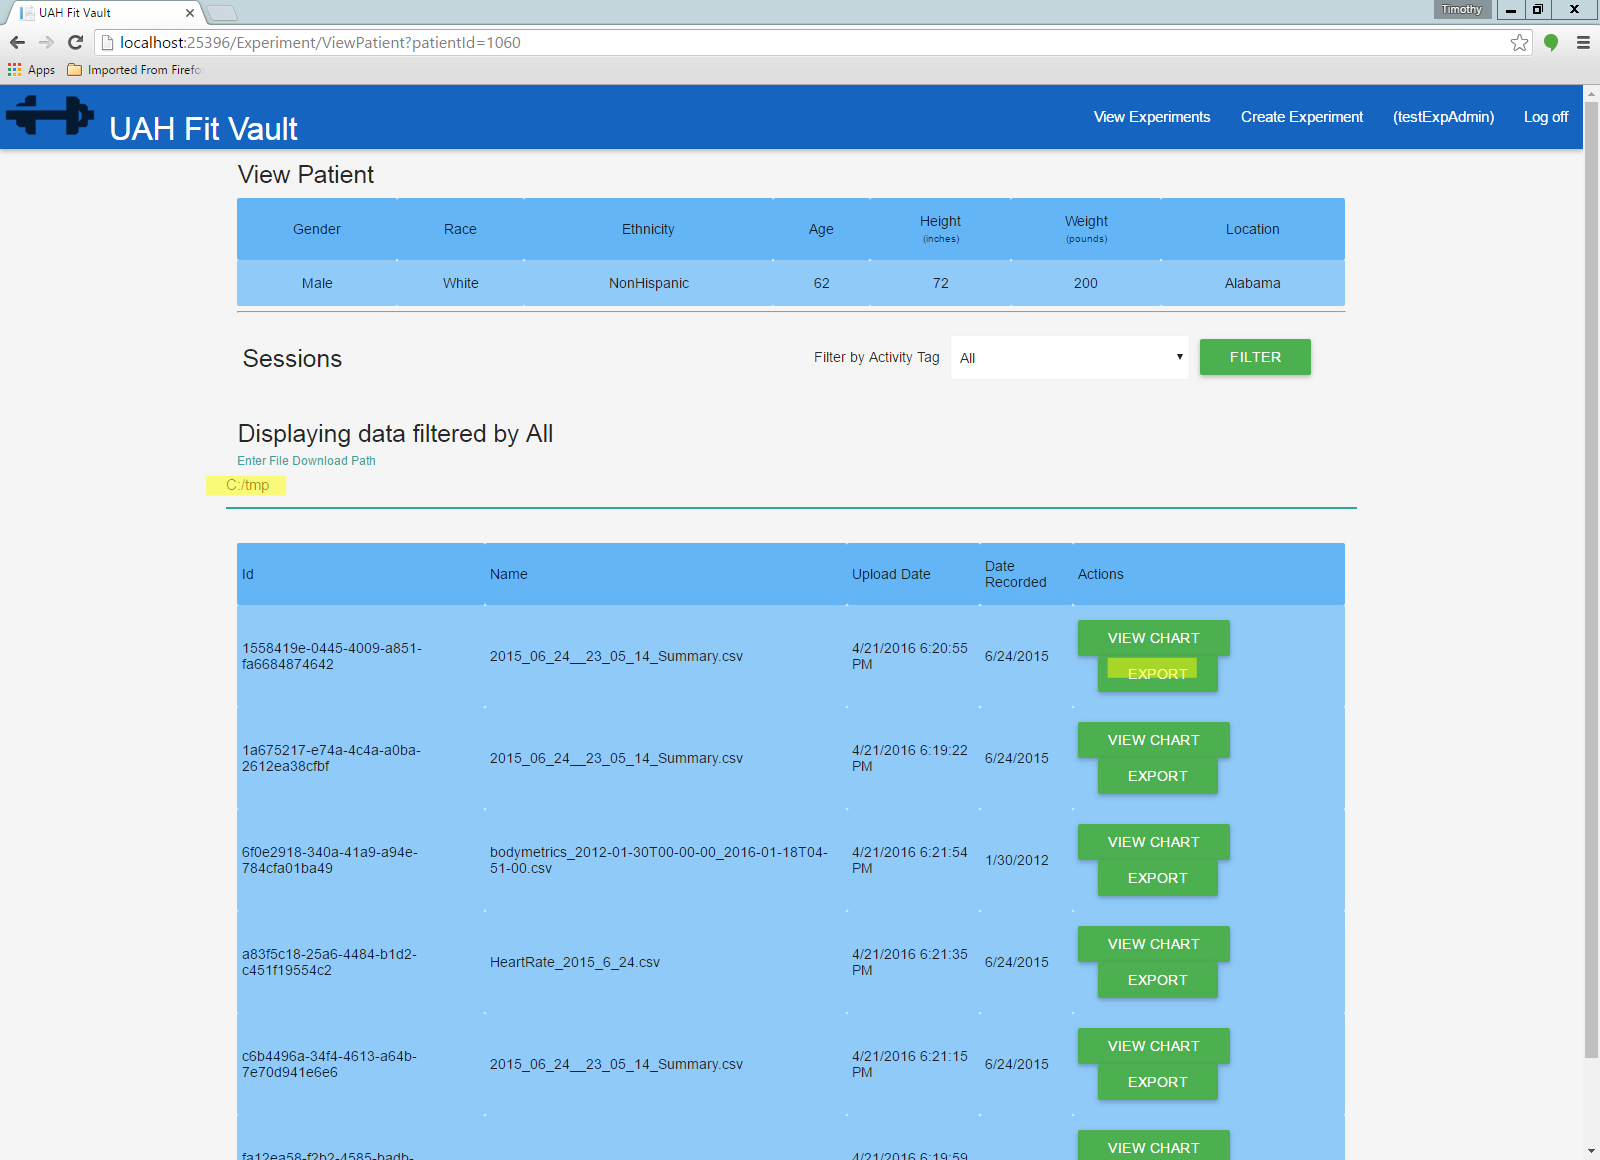
\includegraphics{view_experiments_expadmin_export_3.png}


\subsection{Patient Data Management}
\label{user_guide/patient_data_management:id1}\label{user_guide/patient_data_management::doc}\label{user_guide/patient_data_management:patient-data-management}
Patients have the ability to upload data to the system, view the data they have uploaded, and download that data from
the system at any time.

Contents:


\subsubsection{Patient Data Upload}
\label{user_guide/patient_data_upload:patient-data-upload}\label{user_guide/patient_data_upload::doc}\label{user_guide/patient_data_upload:id1}\setbox0\vbox{
\begin{minipage}{0.95\linewidth}
\textbf{Table of Contents}

\medskip

\begin{itemize}
\item {} 
{\hyperref[user_guide/patient_data_upload:patient-data-upload]{Patient Data Upload}}

\end{itemize}
\end{minipage}}
\begin{center}\setlength{\fboxsep}{5pt}\shadowbox{\box0}\end{center}

A patient can upload data to the system from 3 types of devices:
\begin{itemize}
\item {} 
Zephyr

\item {} 
Basis Peak

\item {} 
Microsoft Band

\end{itemize}

To upload a file, login with your patient account credentials. Then, click on the ``Upload Data'' button at the top
right of the page. This should take you to a screen like this:

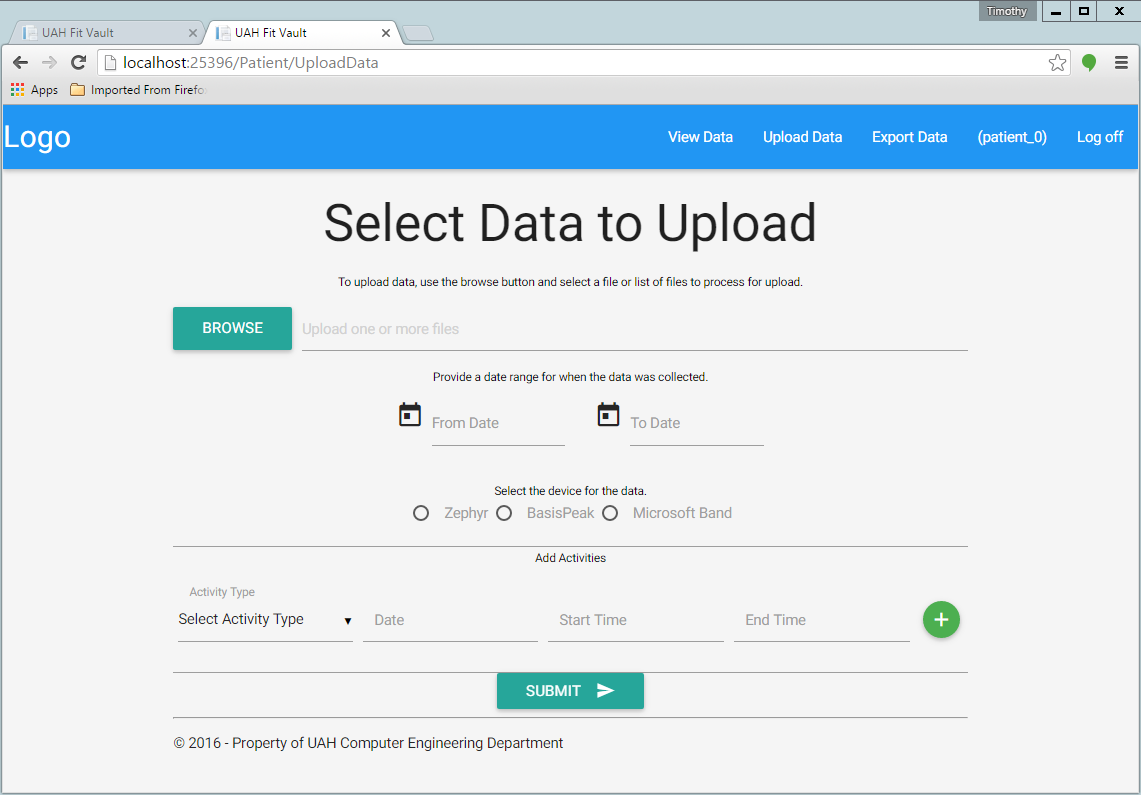
\includegraphics{upload_patient_data.png}

Click the ``BROWSE'' button and follow the wizard to the file(s) you want to upload. Fill in the date of collection
information and select the device type. At this point you can upload data by clicking the ``SUBMIT'' button.

Your Physician may also ask you to fill out activities (the second half of the Upload Data page). Activities must be
set at the time of the data upload. To fill out an activity simply choose an activity type from the ``Activity Type''
dropdown, select the date the activity was performed, and select a start and end time for the activity.

You can input as many activities as you want. To add an activity click the green plus button to the right of the
activity section of the page.


\subsubsection{Patient Data View}
\label{user_guide/patient_data_view:patient-data-view}\label{user_guide/patient_data_view::doc}\label{user_guide/patient_data_view:id1}\setbox0\vbox{
\begin{minipage}{0.95\linewidth}
\textbf{Table of Contents}

\medskip

\begin{itemize}
\item {} 
{\hyperref[user_guide/patient_data_view:patient-data-view]{Patient Data View}}
\begin{itemize}
\item {} 
{\hyperref[user_guide/patient_data_view:physician]{Physician}}

\item {} 
{\hyperref[user_guide/patient_data_view:patient]{Patient}}

\end{itemize}

\end{itemize}
\end{minipage}}
\begin{center}\setlength{\fboxsep}{5pt}\shadowbox{\box0}\end{center}

Both Physicians and Patients can view a patient's data.


\paragraph{Physician}
\label{user_guide/patient_data_view:physician}\label{user_guide/patient_data_view:view-patient-data-physician}
To view patient data as a physician, login with your physician account credentials. Click on the ``Patient Management''
button at the top right of the page. You should then be taken to a page that looks like this:

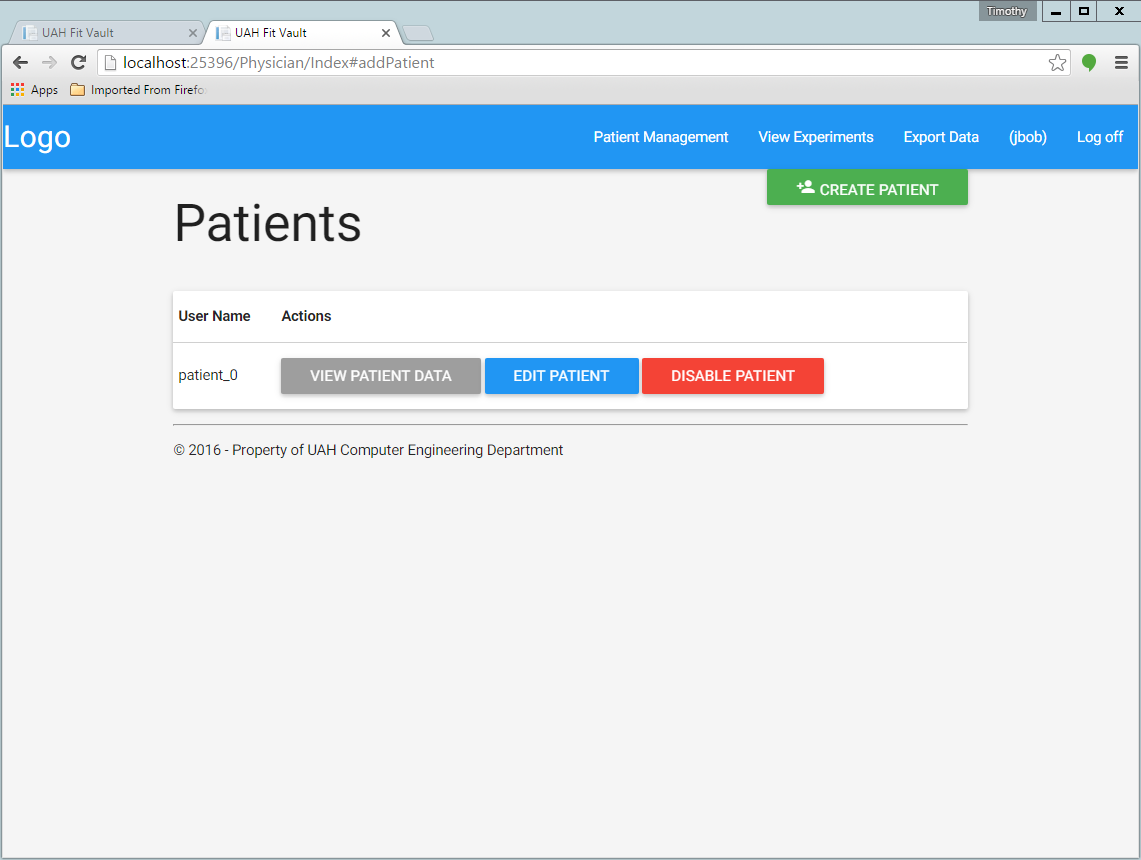
\includegraphics{patient_management.png}

You can then click on the ``VIEW PATIENT DATA'' button for the corresponding patient who's data you want to view. You
will then be taken to a page that looks like this:

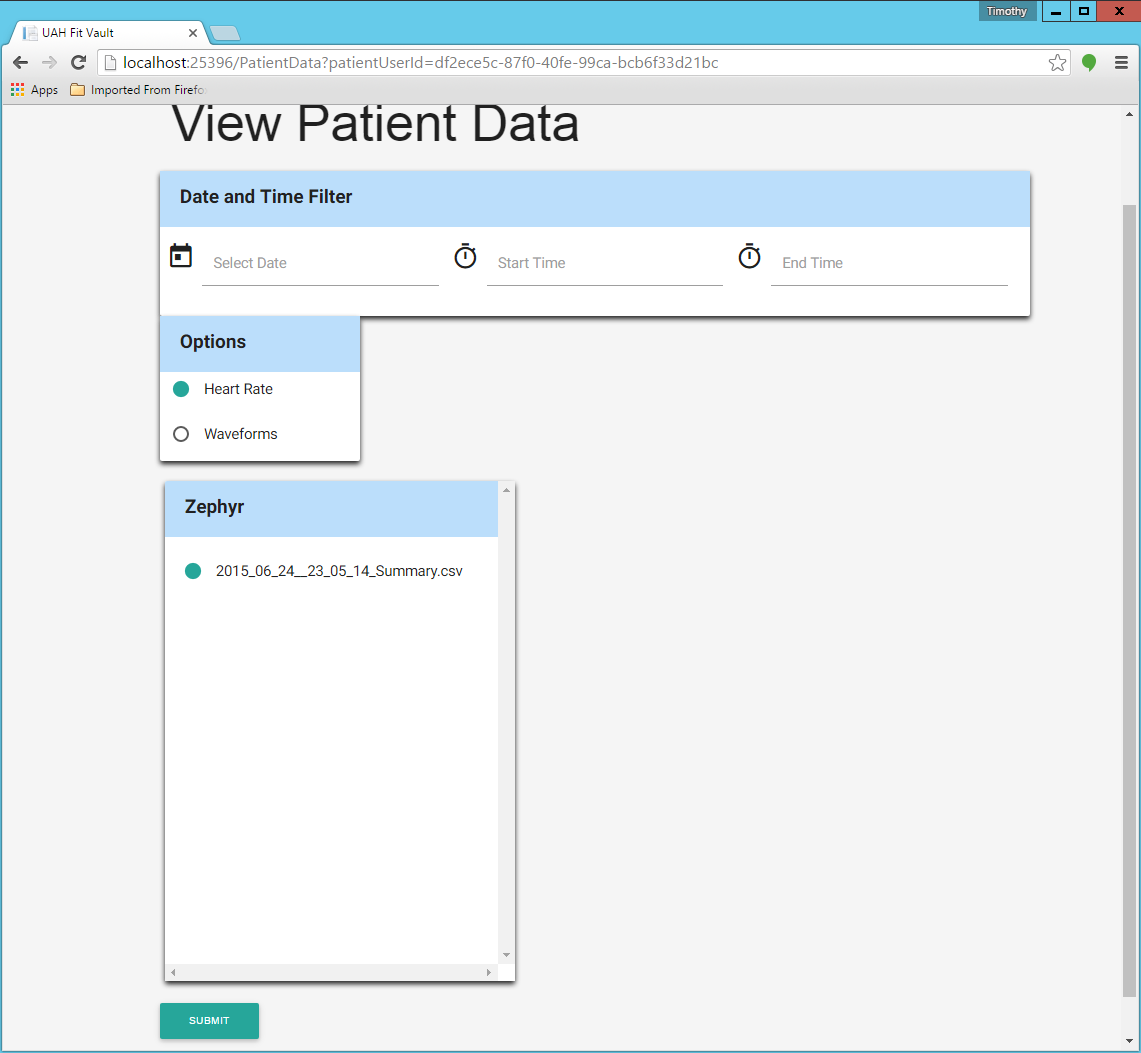
\includegraphics{view_patient_data_physician.png}

You can then select a date and a start time and end time. Then select the file you want to view. Click the ``SUBMIT''
button to display the data at the bottom of the page. It should look like this:

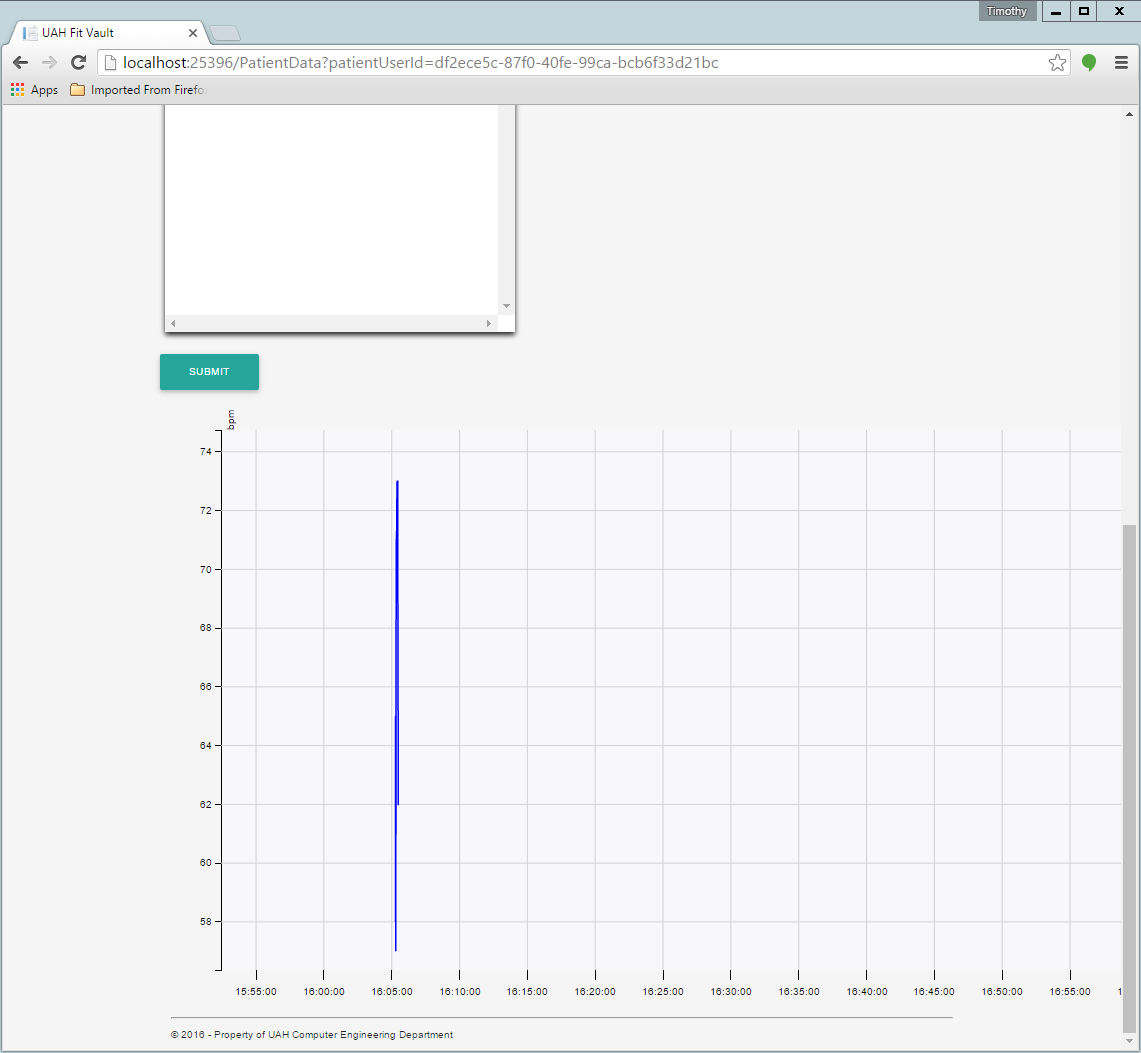
\includegraphics{view_patient_data_physician_2.png}


\paragraph{Patient}
\label{user_guide/patient_data_view:patient}
To view patient data as a patient, login with your patient account credentials. You can then click the ``View Data''
button at the top right of the page. You should then be taken to a page that looks like this:

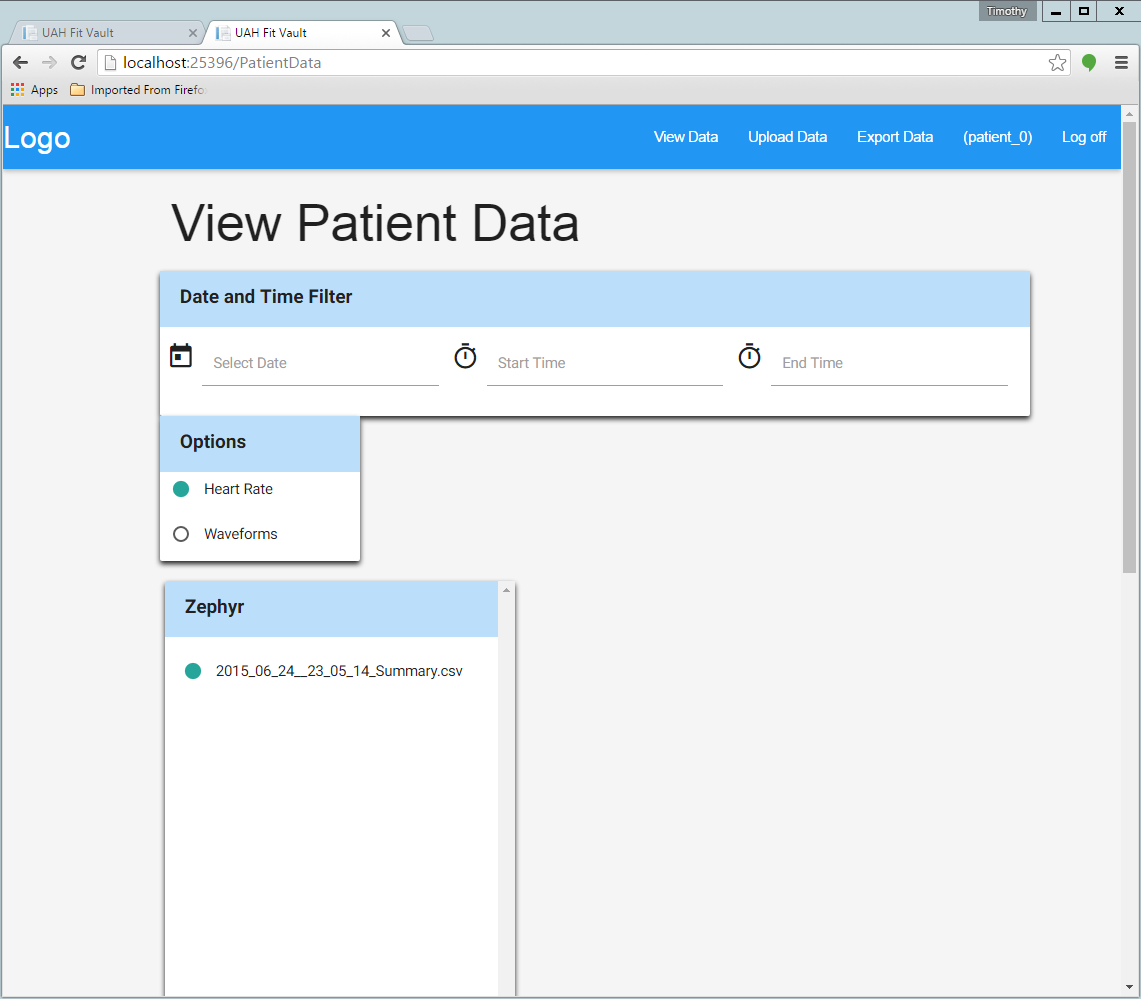
\includegraphics{view_patient_data.png}

You can then select a date and a start time and end time. Then select the file you want to view. Click the ``SUBMIT''
button to display the data at the bottom of the page. It should look like this:

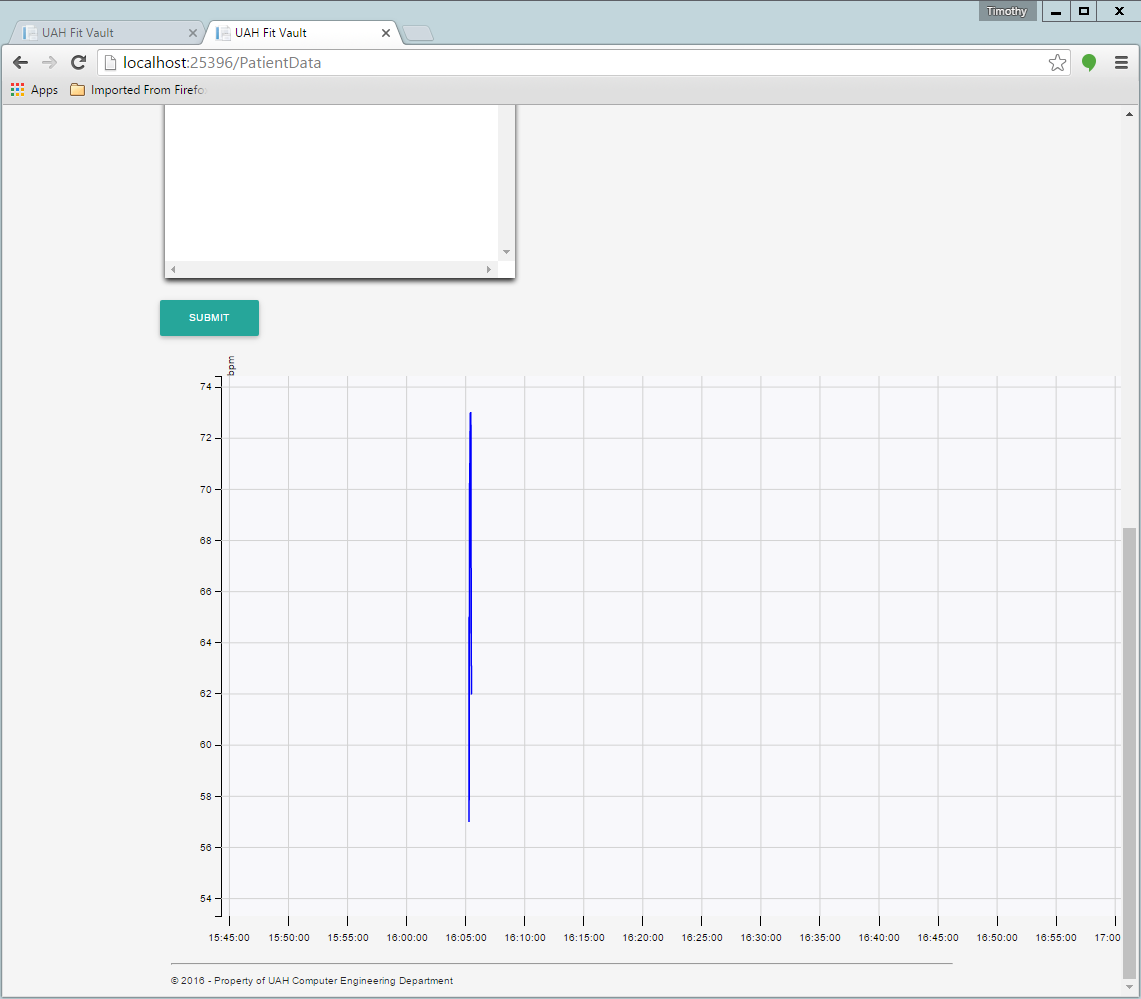
\includegraphics{view_patient_data_2.png}


\subsubsection{Patient Data Download}
\label{user_guide/patient_data_download:patient-data-download}\label{user_guide/patient_data_download::doc}\label{user_guide/patient_data_download:id1}\setbox0\vbox{
\begin{minipage}{0.95\linewidth}
\textbf{Table of Contents}

\medskip

\begin{itemize}
\item {} 
{\hyperref[user_guide/patient_data_download:patient-data-download]{Patient Data Download}}
\begin{itemize}
\item {} 
{\hyperref[user_guide/patient_data_download:patient-account]{Patient Account}}

\end{itemize}

\end{itemize}
\end{minipage}}
\begin{center}\setlength{\fboxsep}{5pt}\shadowbox{\box0}\end{center}

Patients have the ability to export any data they have uploaded.


\paragraph{Patient Account}
\label{user_guide/patient_data_download:patient-account}
Login with your patient credentials. You should see an ``Export Data'' button at the top right of the page. Click on this
button and you will be taken to a page that looks like this:

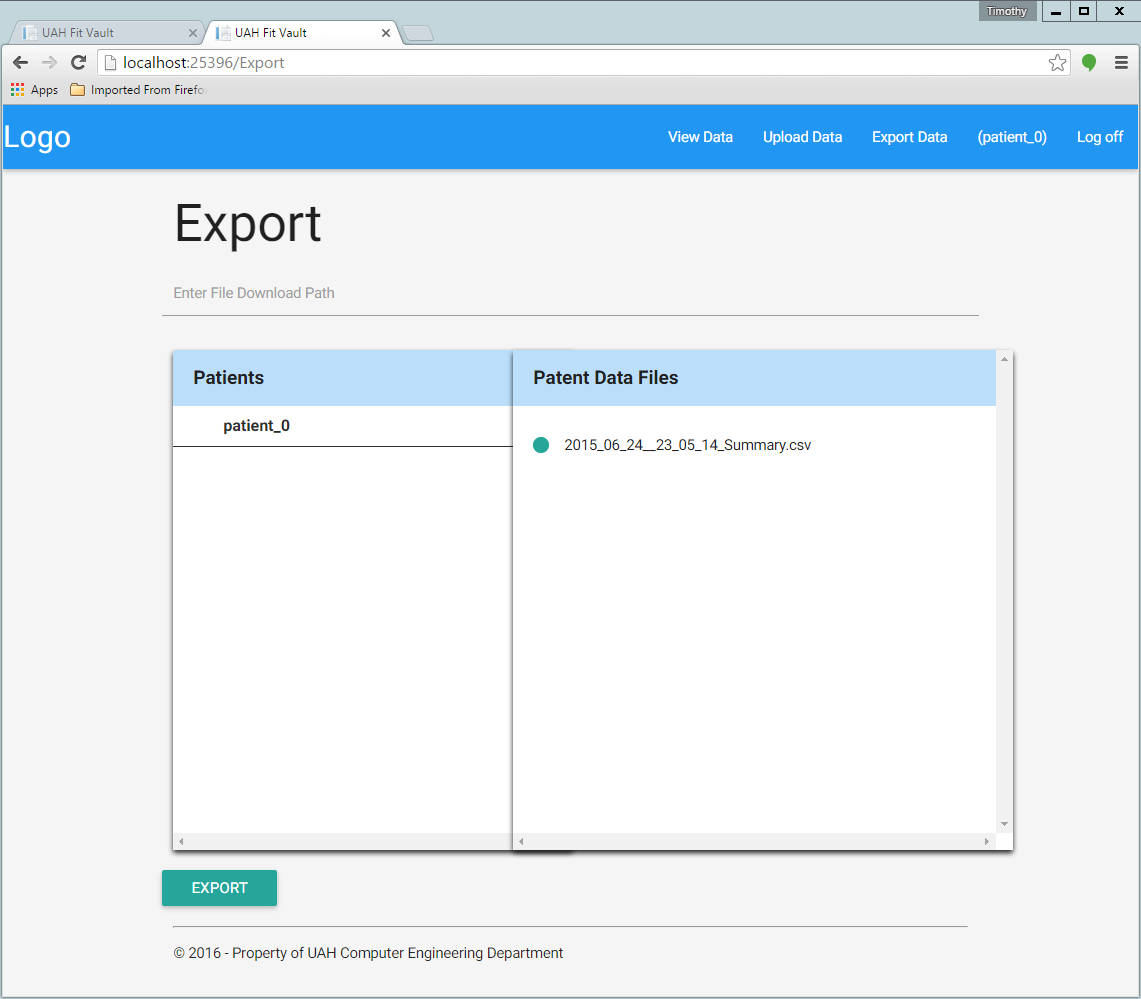
\includegraphics{export_data.png}

Click on your patient account in the ``Patients'' window, then click on the file you want to export in the ``Patient
Data Files'' window. Then simply click the ``EXPORT'' button at the bottom of the page to start the download.


\chapter{UAHealth Bit Vault Software Test Description}
\label{STD/software_test_description:software-test-description}\label{STD/software_test_description:uahealth-bit-vault-software-test-description}\label{STD/software_test_description::doc}\setbox0\vbox{
\begin{minipage}{0.95\linewidth}
\textbf{Table of Contents}

\medskip

\begin{itemize}
\item {} 
{\hyperref[STD/software_test_description:uahealth-bit-vault-software-test-description]{UAHealth Bit Vault Software Test Description}}
\begin{itemize}
\item {} 
{\hyperref[STD/software_test_description:scope]{Scope}}
\begin{itemize}
\item {} 
{\hyperref[STD/software_test_description:identification]{Identification}}

\item {} 
{\hyperref[STD/software_test_description:system-overview]{System Overview}}

\item {} 
{\hyperref[STD/software_test_description:document-overview]{Document Overview}}

\end{itemize}

\item {} 
{\hyperref[STD/software_test_description:referenced-documents]{Referenced Documents}}

\item {} 
{\hyperref[STD/software_test_description:test-descriptions]{Test Descriptions}}
\begin{itemize}
\item {} 
{\hyperref[STD/software_test_description:sign-off]{Sign Off}}

\end{itemize}

\end{itemize}

\end{itemize}
\end{minipage}}
\begin{center}\setlength{\fboxsep}{5pt}\shadowbox{\box0}\end{center}


\section{Scope}
\label{STD/software_test_description:scope}

\subsection{Identification}
\label{STD/software_test_description:identification}
This document shall apply to the final release of the UAHealth Bit Vault Software.


\subsection{System Overview}
\label{STD/software_test_description:system-overview}
The UAHealth Bit Vault Software is designed to be a place for doctors, patients, and administrators to store patient’s
biometric data and run experiments on that data. This is the first deployment of this system.
The software will be deployed on a server in the UAH lab for Dr. Malenkovich. At the end of the development period,
the software will be deployed and ownership shall be transferred to Dr. Malenkovich.


\subsection{Document Overview}
\label{STD/software_test_description:document-overview}
This document is to describe the testing that will be performed on the UAHealth Bit Vault Software for customer acceptance.
Test descriptions and all dependent information are included in this document.


\section{Referenced Documents}
\label{STD/software_test_description:referenced-documents}
None.


\section{Test Descriptions}
\label{STD/software_test_description:test-descriptions}

\subsection{Pytest Tests}
\label{STD/pytest_test_descriptions:pytest-tests}\label{STD/pytest_test_descriptions::doc}\label{STD/pytest_test_descriptions:pytest-test-descriptions}\setbox0\vbox{
\begin{minipage}{0.95\linewidth}
\textbf{Table of Contents}

\medskip

\begin{itemize}
\item {} 
{\hyperref[STD/pytest_test_descriptions:pytest-tests]{Pytest Tests}}
\begin{itemize}
\item {} 
{\hyperref[STD/pytest_test_descriptions:test-preparations]{Test Preparations}}
\begin{itemize}
\item {} 
{\hyperref[STD/pytest_test_descriptions:hardware-preparations]{Hardware Preparations}}

\item {} 
{\hyperref[STD/pytest_test_descriptions:software-preparations]{Software Preparations}}

\item {} 
{\hyperref[STD/pytest_test_descriptions:other-preparations]{Other Preparations}}

\end{itemize}

\item {} 
{\hyperref[STD/pytest_test_descriptions:test-execution]{Test Execution}}

\item {} 
{\hyperref[STD/pytest_test_descriptions:test-details]{Test Details}}

\end{itemize}

\end{itemize}
\end{minipage}}
\begin{center}\setlength{\fboxsep}{5pt}\shadowbox{\box0}\end{center}


\subsubsection{Test Preparations}
\label{STD/pytest_test_descriptions:test-preparations}

\paragraph{Hardware Preparations}
\label{STD/pytest_test_descriptions:hardware-preparations}
In order to run the Pytest tests, you must have a physical computer capable of running the latest distribution of Ubuntu.
Follow the hardware requirements for this distribution. Ubuntu is not required to run the tests, but the hardware
requirements for Ubuntu serve as a minimum requirement to run the Pytest tests.

The computer you use must have access to the UAHealth server in order to run the Pytest tests.
The computer can be the same machine as the UAHealth server, but this is not required.


\paragraph{Software Preparations}
\label{STD/pytest_test_descriptions:software-preparations}
Download the zip file of the github project here: \href{https://github.com/trwq63/med656}{Github} and unzip it in your home directory.

You must have the latest Active Python 3.4 installed on this computer. It can be found here: \href{http://www.activestate.com/activepython/downloads}{Python}. The OS may be Windows
7/2012 or later. If you are using Windows 2012, add ``C:\textbackslash{}Python34'' and ``C:\textbackslash{}Python34\textbackslash{}Scripts'' to your ``Path'' environment variable. You also need to install Firefox. It can be downloaded here: \href{https://www.mozilla.org/en-US/firefox/new/}{Firefox}. The required python packages can be installed by navigating to the project folder and running:

\begin{Verbatim}[commandchars=\\\{\}]
pip install \PYGZhy{}r ./Tests/requirements.txt
\end{Verbatim}


\paragraph{Other Preparations}
\label{STD/pytest_test_descriptions:other-preparations}\label{STD/pytest_test_descriptions:github}

\subsubsection{Test Execution}
\label{STD/pytest_test_descriptions:test-execution}
To run these tests, open a command prompt and navigate to the Tests folder (\textless{}project\_path\textgreater{}/med656/Tests). Then execute
the following command:

py.test -v -s test\_create\_account.py test\_edit\_account.py test\_experiment.py test\_login.py test\_password.py test\_security.py test\_upload.py test\_username.py test\_export.py

The test report will be printed out to the screen. It will display all the tests that were run along with their pass/fail
status.


\subsubsection{Test Details}
\label{STD/pytest_test_descriptions:test-details}
Follow the table below to find details of the test automation.


\paragraph{test\_create\_account module}
\label{STD/test_create_account:test-create-account-module}\label{STD/test_create_account::doc}\label{STD/test_create_account:module-test_create_account}\index{test\_create\_account (module)}
These test cases are designed to test the ability to create and delete accounts
\index{test\_create\_experiment\_admin() (in module test\_create\_account)}

\begin{fulllineitems}
\phantomsection\label{STD/test_create_account:test_create_account.test_create_experiment_admin}\pysiglinewithargsret{\code{test\_create\_account.}\bfcode{test\_create\_experiment\_admin}}{\emph{logoff}}{}
\textbf{Requirements:}
\begin{itemize}
\item {} 
3.1.1.1.3.1: minimum information stored for experiment admin account

\item {} 
3.1.1.1.4.2: System Administrators shall be able to enable users

\item {} 
3.1.1.7: Experiment administrators create their own accounts

\item {} 
3.1.1.7.1: System Administrators shall verify the creation of a experiment admin account

\item {} 
3.1.6: The system shall provide account management.

\item {} 
3.1.6.1: The system shall allow account creation

\item {} 
3.1.6.1.1: The system shall force account approval for experiment admins

\item {} 
3.1.1.4: System requires a minimum security criteria

\item {} 
3.1.1.4.1: Password must be at least 10 characters

\item {} 
3.1.1.4.2: Password shall contain at least 1 upper and 1 lower case character

\item {} 
3.1.1.4.3: Password shall contain at least 1 number

\item {} 
3.1.1.4.4: Password shall contain at least 1 special character

\end{itemize}

\textbf{Pre Conditions:}
\begin{itemize}
\item {} 
logoff fixture

\end{itemize}

\textbf{Input:}
\begin{itemize}
\item {} 
user = `awong'

\item {} 
pwd = \href{mailto:'P@ssword10}{`P@ssword10}`

\item {} 
email = \href{mailto:'awong@futurama.com}{`awong@futurama.com}`

\item {} 
first\_name = `Amy'

\item {} 
last\_name = `Wong'

\item {} 
address = `304 Wherever Street, New New York City, New New York'

\item {} 
phone\_number = `123-456-7890'

\end{itemize}

\begin{tabulary}{\linewidth}{|L|L|L|}
\hline
\textsf{\relax 
Steps
} & \textsf{\relax 
Expected Result
} & \textsf{\relax 
Actual Result
}\\
\hline
request account
 & 
Request confirmed
 & \\
\hline
approve account
 & 
Admin can approve
 & \\
\hline
login
 & 
User can login
 & \\
\hline\end{tabulary}


\end{fulllineitems}

\index{test\_create\_patient() (in module test\_create\_account)}

\begin{fulllineitems}
\phantomsection\label{STD/test_create_account:test_create_account.test_create_patient}\pysiglinewithargsret{\code{test\_create\_account.}\bfcode{test\_create\_patient}}{\emph{login\_tphysician}}{}
\textbf{Requirements:}
\begin{itemize}
\item {} 
3.1.1.1.1.1: minimum information stored for patient account

\item {} 
3.1.1.1.2.5: Physician user can add a patient to the system

\item {} 
3.1.1.3.1: Display patient ID to physician at the time of creation

\item {} 
3.1.1.7.2: Physicians shall create their patients accounts

\item {} 
3.1.6: The system shall provide account management.

\item {} 
3.1.6.1: The system shall allow account creation

\item {} 
3.1.6.1.2: Patients shall not need approval for account creation

\item {} 
3.1.1.4: System requires a minimum security criteria

\item {} 
3.1.1.4.1: Password must be at least 10 characters

\item {} 
3.1.1.4.2: Password shall contain at least 1 upper and 1 lower case character

\item {} 
3.1.1.4.3: Password shall contain at least 1 number

\item {} 
3.1.1.4.4: Password shall contain at least 1 special character

\end{itemize}

\textbf{Pre Conditions:}
\begin{itemize}
\item {} 
login\_tphysician fixture

\end{itemize}

\textbf{Input:}
\begin{itemize}
\item {} 
user = `testPatientCreate\_\textless{}random number\textgreater{}'

\item {} 
pwd = \href{mailto:'P@ssword10}{`P@ssword10}`

\item {} 
byear = `1954'

\item {} 
bmonth = `March'

\item {} 
bday = `3'

\item {} 
loc = `Alabama'

\item {} 
wght = `200'

\item {} 
hght = `72'

\item {} 
gen = `male'

\item {} 
race = `white'

\item {} 
eth = `non\_hispanic'

\item {} 
physician = `testPhysician'

\end{itemize}

\begin{tabulary}{\linewidth}{|L|L|L|}
\hline
\textsf{\relax 
Steps
} & \textsf{\relax 
Expected Result
} & \textsf{\relax 
Actual Result
}\\
\hline
create patient account
 & 
No error msgs
 & \\
\hline
login as patient
 & 
Patient can login
 & \\
\hline\end{tabulary}


\end{fulllineitems}

\index{test\_create\_physician() (in module test\_create\_account)}

\begin{fulllineitems}
\phantomsection\label{STD/test_create_account:test_create_account.test_create_physician}\pysiglinewithargsret{\code{test\_create\_account.}\bfcode{test\_create\_physician}}{\emph{logoff}}{}
\textbf{Requirements:}
\begin{itemize}
\item {} 
3.1.1.1.2.1: minimum information stored for physician account

\item {} 
3.1.1.1.4.2: System Administrators shall be able to enable users

\item {} 
3.1.1.7: Physicians create their own accounts

\item {} 
3.1.1.7.1: System Administrators shall verify the creation of a physician account

\item {} 
3.1.6: The system shall provide account management.

\item {} 
3.1.6.1: The system shall allow account creation

\item {} 
3.1.6.1.1: The system shall force account approval for physicians

\item {} 
3.1.1.4: System requires a minimum security criteria

\item {} 
3.1.1.4.1: Password must be at least 10 characters

\item {} 
3.1.1.4.2: Password shall contain at least 1 upper and 1 lower case character

\item {} 
3.1.1.4.3: Password shall contain at least 1 number

\item {} 
3.1.1.4.4: Password shall contain at least 1 special character

\end{itemize}

\textbf{Pre Conditions:}
\begin{itemize}
\item {} 
logoff fixture

\end{itemize}

\textbf{Input:}
\begin{itemize}
\item {} 
user = `hfarnswroth'

\item {} 
pwd = \href{mailto:'P@ssword10}{`P@ssword10}`

\item {} 
email = \href{mailto:'hfarnsworth@futurama.com}{`hfarnsworth@futurama.com}`

\item {} 
first\_name = `Hubert'

\item {} 
last\_name = `Farnsworth'

\item {} 
address = `304 Wherever Street, New New York City, New New York'

\item {} 
phone\_number = `123-456-7890'

\end{itemize}

\begin{tabulary}{\linewidth}{|L|L|L|}
\hline
\textsf{\relax 
Steps
} & \textsf{\relax 
Expected Result
} & \textsf{\relax 
Actual Result
}\\
\hline
request account
 & 
Request confirmed
 & \\
\hline
approve account
 & 
Admin can approve
 & \\
\hline
login
 & 
User can login
 & \\
\hline\end{tabulary}


\end{fulllineitems}

\index{test\_create\_system\_admin() (in module test\_create\_account)}

\begin{fulllineitems}
\phantomsection\label{STD/test_create_account:test_create_account.test_create_system_admin}\pysiglinewithargsret{\code{test\_create\_account.}\bfcode{test\_create\_system\_admin}}{\emph{login\_sysadmin}}{}
\textbf{Requirements:}
\begin{itemize}
\item {} 
3.1.1.1.4.1: minimum information stored for experiment admin account

\item {} 
3.1.1.1.4.2: System Administrators shall be able to enable users

\item {} 
3.1.6: The system shall provide account management.

\item {} 
3.1.6.1: The system shall allow account creation

\item {} 
3.1.1.4: System requires a minimum security criteria

\item {} 
3.1.1.4.1: Password must be at least 10 characters

\item {} 
3.1.1.4.2: Password shall contain at least 1 upper and 1 lower case character

\item {} 
3.1.1.4.3: Password shall contain at least 1 number

\item {} 
3.1.1.4.4: Password shall contain at least 1 special character

\end{itemize}

\textbf{Pre Conditions:}
\begin{itemize}
\item {} 
logoff fixture

\end{itemize}

\textbf{Input:}
\begin{itemize}
\item {} 
user = `lnibbler'

\item {} 
pwd = \href{mailto:'P@ssword10}{`P@ssword10}`

\item {} 
email = \href{mailto:'lnibbler@futurama.com}{`lnibbler@futurama.com}`

\end{itemize}

\begin{tabulary}{\linewidth}{|L|L|L|}
\hline
\textsf{\relax 
Steps
} & \textsf{\relax 
Expected Result
} & \textsf{\relax 
Actual Result
}\\
\hline
Login as fitadmin
 & 
Login Successful
 & \\
\hline
Create another system admin
 & 
No errors
 & \\
\hline
login as new system admin
 & 
User can login
 & \\
\hline\end{tabulary}


\end{fulllineitems}

\index{test\_delete\_experiment\_admin() (in module test\_create\_account)}

\begin{fulllineitems}
\phantomsection\label{STD/test_create_account:test_create_account.test_delete_experiment_admin}\pysiglinewithargsret{\code{test\_create\_account.}\bfcode{test\_delete\_experiment\_admin}}{\emph{logoff}}{}
\textbf{Requirements:}
\begin{itemize}
\item {} 
3.1.6.3: System administrator can delete accounts

\item {} 
3.1.6: The system shall provide account management.

\end{itemize}

\textbf{Pre Conditions:}
\begin{itemize}
\item {} 
logoff fixture

\end{itemize}

\textbf{Input:}
\begin{itemize}
\item {} 
user = `awong'

\item {} 
username = `Amy Wong'

\item {} 
pwd = \href{mailto:'P@ssword10}{`P@ssword10}`

\end{itemize}

\begin{tabulary}{\linewidth}{|L|L|L|}
\hline
\textsf{\relax 
Steps
} & \textsf{\relax 
Expected Result
} & \textsf{\relax 
Actual Result
}\\
\hline
delete experiment admin account
 & 
No error msgs
 & \\
\hline
login as patient
 & 
User cannot login
 & \\
\hline\end{tabulary}


\end{fulllineitems}

\index{test\_delete\_patient() (in module test\_create\_account)}

\begin{fulllineitems}
\phantomsection\label{STD/test_create_account:test_create_account.test_delete_patient}\pysiglinewithargsret{\code{test\_create\_account.}\bfcode{test\_delete\_patient}}{\emph{logoff}}{}
\textbf{Requirements:}
\begin{itemize}
\item {} 
3.1.1.1.2.6: Physicians can delete patients

\end{itemize}

\textbf{Pre Conditions:}
\begin{itemize}
\item {} 
logoff fixture

\end{itemize}

\textbf{Input:}
\begin{itemize}
\item {} 
user = `pfry'

\item {} 
pwd = \href{mailto:'P@ssword10}{`P@ssword10}`

\item {} 
phy = `testPhysician'

\item {} 
phy\_pass = \href{mailto:'P@ssword10}{`P@ssword10}`

\end{itemize}

\begin{tabulary}{\linewidth}{|L|L|L|}
\hline
\textsf{\relax 
Steps
} & \textsf{\relax 
Expected Result
} & \textsf{\relax 
Actual Result
}\\
\hline
delete patient account
 & 
No error msgs
 & \\
\hline
login as patient
 & 
Patient cannot login
 & \\
\hline\end{tabulary}


\end{fulllineitems}

\index{test\_delete\_physician() (in module test\_create\_account)}

\begin{fulllineitems}
\phantomsection\label{STD/test_create_account:test_create_account.test_delete_physician}\pysiglinewithargsret{\code{test\_create\_account.}\bfcode{test\_delete\_physician}}{\emph{logoff}}{}
\textbf{Requirements:}
\begin{itemize}
\item {} 
3.1.6.3: System administrator can delete accounts

\item {} 
3.1.6: The system shall provide account management.

\end{itemize}

\textbf{Pre Conditions:}
\begin{itemize}
\item {} 
logoff fixture

\end{itemize}

\textbf{Input:}
\begin{itemize}
\item {} 
user = `hfarnswroth'

\item {} 
username = `Hubert Farnsworth'

\item {} 
pwd = \href{mailto:'P@ssword10}{`P@ssword10}`

\end{itemize}

\begin{tabulary}{\linewidth}{|L|L|L|}
\hline
\textsf{\relax 
Steps
} & \textsf{\relax 
Expected Result
} & \textsf{\relax 
Actual Result
}\\
\hline
delete physician account
 & 
No error msgs
 & \\
\hline
login as patient
 & 
User cannot login
 & \\
\hline\end{tabulary}


\end{fulllineitems}



\paragraph{test\_edit\_account module}
\label{STD/test_edit_account:test-edit-account-module}\label{STD/test_edit_account:module-test_edit_account}\label{STD/test_edit_account::doc}\index{test\_edit\_account (module)}
These tests are here to verify that the accounts can have their information edited.
\index{test\_physician\_can\_edit\_his\_account() (in module test\_edit\_account)}

\begin{fulllineitems}
\phantomsection\label{STD/test_edit_account:test_edit_account.test_physician_can_edit_his_account}\pysiglinewithargsret{\code{test\_edit\_account.}\bfcode{test\_physician\_can\_edit\_his\_account}}{\emph{login\_tphysician}}{}
\textbf{Requirements:}
\begin{itemize}
\item {} 
3.1.1.1.2.2: Physician can update his account

\item {} 
3.1.6.2: System shall allow users to edit their account

\end{itemize}

\textbf{Pre Conditions:}
\begin{itemize}
\item {} 
login\_tphysician fixture

\end{itemize}

\textbf{Input:}

\begin{tabulary}{\linewidth}{|L|L|L|}
\hline
\textsf{\relax 
Steps
} & \textsf{\relax 
Expected Result
} & \textsf{\relax 
Actual Result
}\\
\hline
Go to management page
 & 
No Errors
 & \\
\hline
Change the email address
 & 
No Errors
 & \\
\hline
Check the email address
 & 
Email has changed
 & \\
\hline\end{tabulary}


\end{fulllineitems}



\paragraph{test\_login module}
\label{STD/test_login:test-login-module}\label{STD/test_login:module-test_login}\label{STD/test_login::doc}\index{test\_login (module)}
These tests are to verify that the accounts can be logged into
\index{test\_login\_bad\_pass() (in module test\_login)}

\begin{fulllineitems}
\phantomsection\label{STD/test_login:test_login.test_login_bad_pass}\pysiglinewithargsret{\code{test\_login.}\bfcode{test\_login\_bad\_pass}}{\emph{logoff}}{}
\textbf{Requirements:}
\begin{itemize}
\item {} 
3.1.1: System shall provide user authentication

\end{itemize}

\textbf{Pre Conditions:}
\begin{itemize}
\item {} 
logoff fixture

\end{itemize}

\textbf{Input:}
\begin{itemize}
\item {} 
user = `testPhysician'

\item {} 
password = `!nc0rrect'

\item {} 
expected = `Invalid login attempt.'

\end{itemize}

\textbf{Expected Results:}

User `testPhysician' sees the home page after logging in

\begin{tabulary}{\linewidth}{|L|L|L|}
\hline
\textsf{\relax 
Steps
} & \textsf{\relax 
Expected Result
} & \textsf{\relax 
Actual Result
}\\
\hline
login
 & 
Invalid login
 & \\
\hline\end{tabulary}


\end{fulllineitems}

\index{test\_login\_bad\_user() (in module test\_login)}

\begin{fulllineitems}
\phantomsection\label{STD/test_login:test_login.test_login_bad_user}\pysiglinewithargsret{\code{test\_login.}\bfcode{test\_login\_bad\_user}}{\emph{logoff}}{}
\textbf{Requirements:}
\begin{itemize}
\item {} 
3.1.1: System shall provide user authentication

\end{itemize}

\textbf{Pre Conditions:}
\begin{itemize}
\item {} 
logoff fixture

\end{itemize}

\textbf{Input:}
\begin{itemize}
\item {} 
user = `fake'

\item {} 
password = \href{mailto:'P@ssword10}{`P@ssword10}`

\item {} 
expected = `Invalid login attempt.'

\end{itemize}

\textbf{Expected Results:}

User `testPhysician' sees the home page after logging in

\begin{tabulary}{\linewidth}{|L|L|L|}
\hline
\textsf{\relax 
Steps
} & \textsf{\relax 
Expected Result
} & \textsf{\relax 
Actual Result
}\\
\hline
login
 & 
Invalid login
 & \\
\hline\end{tabulary}


\end{fulllineitems}

\index{test\_login\_experiment\_admin() (in module test\_login)}

\begin{fulllineitems}
\phantomsection\label{STD/test_login:test_login.test_login_experiment_admin}\pysiglinewithargsret{\code{test\_login.}\bfcode{test\_login\_experiment\_admin}}{\emph{logoff}}{}
\textbf{Requirements:}
\begin{itemize}
\item {} 
3.1.1: System shall provide user authentication

\item {} 
3.1.1.5: System shall allow user to log out of account

\end{itemize}

\textbf{Pre Conditions:}
\begin{itemize}
\item {} 
logoff fixture

\end{itemize}

\textbf{Input:}
\begin{itemize}
\item {} 
user = `testExpAdmin'

\item {} 
password = \href{mailto:'P@ssword10}{`P@ssword10}`

\end{itemize}

\textbf{Expected Results:}

User `testPhysician' sees the home page after logging in

\begin{tabulary}{\linewidth}{|L|L|L|}
\hline
\textsf{\relax 
Steps
} & \textsf{\relax 
Expected Result
} & \textsf{\relax 
Actual Result
}\\
\hline
login
 & 
Login Success!
 & \\
\hline\end{tabulary}


\end{fulllineitems}

\index{test\_login\_patient() (in module test\_login)}

\begin{fulllineitems}
\phantomsection\label{STD/test_login:test_login.test_login_patient}\pysiglinewithargsret{\code{test\_login.}\bfcode{test\_login\_patient}}{\emph{logoff}, \emph{test\_patients}}{}
\textbf{Requirements:}
\begin{itemize}
\item {} 
3.1.1: System shall provide user authentication

\item {} 
3.1.1.5: System shall allow user to log out of account

\end{itemize}

\textbf{Pre Conditions:}
\begin{itemize}
\item {} 
logoff fixture

\end{itemize}

\textbf{Input:}
\begin{itemize}
\item {} 
user = `testPatient'

\item {} 
password = \href{mailto:'P@ssword10}{`P@ssword10}`

\end{itemize}

\textbf{Expected Results:}

User `testPhysician' sees the home page after logging in

\begin{tabulary}{\linewidth}{|L|L|L|}
\hline
\textsf{\relax 
Steps
} & \textsf{\relax 
Expected Result
} & \textsf{\relax 
Actual Result
}\\
\hline
login
 & 
Login Success!
 & \\
\hline\end{tabulary}


\end{fulllineitems}

\index{test\_login\_physician() (in module test\_login)}

\begin{fulllineitems}
\phantomsection\label{STD/test_login:test_login.test_login_physician}\pysiglinewithargsret{\code{test\_login.}\bfcode{test\_login\_physician}}{\emph{logoff}}{}
\textbf{Requirements:}
\begin{itemize}
\item {} 
3.1.1: System shall provide user authentication

\item {} 
3.1.1.5: System shall allow user to log out of account

\end{itemize}

\textbf{Pre Conditions:}
\begin{itemize}
\item {} 
logoff fixture

\end{itemize}

\textbf{Input:}
\begin{itemize}
\item {} 
user = `testPhysician'

\item {} 
password = \href{mailto:'P@ssword10}{`P@ssword10}`

\end{itemize}

\textbf{Expected Results:}

User `testPhysician' sees the home page after logging in

\begin{tabulary}{\linewidth}{|L|L|L|}
\hline
\textsf{\relax 
Steps
} & \textsf{\relax 
Expected Result
} & \textsf{\relax 
Actual Result
}\\
\hline
login
 & 
Login Success!
 & \\
\hline\end{tabulary}


\end{fulllineitems}

\index{test\_login\_system\_admin() (in module test\_login)}

\begin{fulllineitems}
\phantomsection\label{STD/test_login:test_login.test_login_system_admin}\pysiglinewithargsret{\code{test\_login.}\bfcode{test\_login\_system\_admin}}{\emph{logoff}}{}
\textbf{Requirements:}
\begin{itemize}
\item {} 
3.1.1: System shall provide user authentication

\item {} 
3.1.1.5: System shall allow user to log out of account

\end{itemize}

\textbf{Pre Conditions:}
\begin{itemize}
\item {} 
logoff fixture

\end{itemize}

\textbf{Input:}
\begin{itemize}
\item {} 
user = `fitadmin'

\item {} 
password = `Password1!'

\end{itemize}

\textbf{Expected Results:}

User `testPhysician' sees the home page after logging in

\begin{tabulary}{\linewidth}{|L|L|L|}
\hline
\textsf{\relax 
Steps
} & \textsf{\relax 
Expected Result
} & \textsf{\relax 
Actual Result
}\\
\hline
login
 & 
Login Success!
 & \\
\hline\end{tabulary}


\end{fulllineitems}



\paragraph{test\_password module}
\label{STD/test_password:test-password-module}\label{STD/test_password:module-test_password}\label{STD/test_password::doc}\index{test\_password (module)}
These tests are to make sure password functionality meets the requirements
\index{test\_password\_case() (in module test\_password)}

\begin{fulllineitems}
\phantomsection\label{STD/test_password:test_password.test_password_case}\pysiglinewithargsret{\code{test\_password.}\bfcode{test\_password\_case}}{\emph{logoff}}{}
\textbf{Requirements:}
\begin{itemize}
\item {} 
3.1.1.4: System requires a minimum security criteria

\item {} 
3.1.1.4.2: Password shall contain at least 1 upper and 1 lower case character

\end{itemize}

\textbf{Pre Conditions:}
\begin{itemize}
\item {} 
logoff fixture

\end{itemize}

\textbf{Input:}
\begin{itemize}
\item {} 
user = `pfry'

\item {} 
pwd = \href{mailto:'p@ssword10}{`p@ssword10}`

\item {} 
email = \href{mailto:'pfry@futurama.com}{`pfry@futurama.com}`

\item {} 
first\_name = `Fry'

\item {} 
last\_name = `Phillip'

\item {} 
address = `304 Wherever Street, New New York City, New New York'

\item {} 
phone\_number = `123-456-7890'

\end{itemize}

\begin{tabulary}{\linewidth}{|L|L|L|}
\hline
\textsf{\relax 
Steps
} & \textsf{\relax 
Expected Result
} & \textsf{\relax 
Actual Result
}\\
\hline
request account
 & 
password case error
 & \\
\hline\end{tabulary}


\end{fulllineitems}

\index{test\_password\_digit() (in module test\_password)}

\begin{fulllineitems}
\phantomsection\label{STD/test_password:test_password.test_password_digit}\pysiglinewithargsret{\code{test\_password.}\bfcode{test\_password\_digit}}{\emph{logoff}}{}
\textbf{Requirements:}
\begin{itemize}
\item {} 
3.1.1.4: System requires a minimum security criteria

\item {} 
3.1.1.4.3: Password shall contain at least 1 number

\end{itemize}

\textbf{Pre Conditions:}
\begin{itemize}
\item {} 
logoff fixture

\end{itemize}

\textbf{Input:}
\begin{itemize}
\item {} 
user = `pfry'

\item {} 
pwd = \href{mailto:'P@ssworddd}{`P@ssworddd}`

\item {} 
email = \href{mailto:'pfry@futurama.com}{`pfry@futurama.com}`

\item {} 
first\_name = `Fry'

\item {} 
last\_name = `Phillip'

\item {} 
address = `304 Wherever Street, New New York City, New New York'

\item {} 
phone\_number = `123-456-7890'

\end{itemize}

\begin{tabulary}{\linewidth}{|L|L|L|}
\hline
\textsf{\relax 
Steps
} & \textsf{\relax 
Expected Result
} & \textsf{\relax 
Actual Result
}\\
\hline
request account
 & 
password digit error
 & \\
\hline\end{tabulary}


\end{fulllineitems}

\index{test\_password\_length() (in module test\_password)}

\begin{fulllineitems}
\phantomsection\label{STD/test_password:test_password.test_password_length}\pysiglinewithargsret{\code{test\_password.}\bfcode{test\_password\_length}}{\emph{logoff}}{}
\textbf{Requirements:}
\begin{itemize}
\item {} 
3.1.1.4: System requires a minimum security criteria

\item {} 
3.1.1.4.1: Password must be at least 10 characters

\end{itemize}

\textbf{Pre Conditions:}
\begin{itemize}
\item {} 
logoff fixture

\end{itemize}

\textbf{Input:}
\begin{itemize}
\item {} 
user = `pfry'

\item {} 
pwd = \href{mailto:'P@ssword1}{`P@ssword1}`

\item {} 
email = \href{mailto:'pfry@futurama.com}{`pfry@futurama.com}`

\item {} 
first\_name = `Fry'

\item {} 
last\_name = `Phillip'

\item {} 
address = `304 Wherever Street, New New York City, New New York'

\item {} 
phone\_number = `123-456-7890'

\end{itemize}

\begin{tabulary}{\linewidth}{|L|L|L|}
\hline
\textsf{\relax 
Steps
} & \textsf{\relax 
Expected Result
} & \textsf{\relax 
Actual Result
}\\
\hline
request account
 & 
password length error
 & \\
\hline\end{tabulary}


\end{fulllineitems}

\index{test\_password\_special\_char() (in module test\_password)}

\begin{fulllineitems}
\phantomsection\label{STD/test_password:test_password.test_password_special_char}\pysiglinewithargsret{\code{test\_password.}\bfcode{test\_password\_special\_char}}{\emph{logoff}}{}
\textbf{Requirements:}
\begin{itemize}
\item {} 
3.1.1.4: System requires a minimum security criteria

\item {} 
3.1.1.4.4: Password shall contain at least 1 special character

\end{itemize}

\textbf{Pre Conditions:}
\begin{itemize}
\item {} 
logoff fixture

\end{itemize}

\textbf{Input:}
\begin{itemize}
\item {} 
user = `pfry'

\item {} 
pwd = `Password10'

\item {} 
email = \href{mailto:'pfry@futurama.com}{`pfry@futurama.com}`

\item {} 
first\_name = `Fry'

\item {} 
last\_name = `Phillip'

\item {} 
address = `304 Wherever Street, New New York City, New New York'

\item {} 
phone\_number = `123-456-7890'

\end{itemize}

\begin{tabulary}{\linewidth}{|L|L|L|}
\hline
\textsf{\relax 
Steps
} & \textsf{\relax 
Expected Result
} & \textsf{\relax 
Actual Result
}\\
\hline
request account
 & 
password digit error
 & \\
\hline\end{tabulary}


\end{fulllineitems}

\index{test\_reset\_password() (in module test\_password)}

\begin{fulllineitems}
\phantomsection\label{STD/test_password:test_password.test_reset_password}\pysiglinewithargsret{\code{test\_password.}\bfcode{test\_reset\_password}}{\emph{login\_sysadmin}}{}
\textbf{Requirements:}
\begin{itemize}
\item {} 
3.1.1.1.4.3: System Administrators can reset passwords

\end{itemize}

\textbf{Pre Conditions:}
\begin{itemize}
\item {} 
login\_sysadmin fixture

\end{itemize}

\textbf{Input:}
\begin{itemize}
\item {} 
user = `testPhysician2'

\item {} 
username = `test physician2'

\item {} 
pwd = `Password1!'

\end{itemize}

\begin{tabulary}{\linewidth}{|L|L|L|}
\hline
\textsf{\relax 
Steps
} & \textsf{\relax 
Expected Result
} & \textsf{\relax 
Actual Result
}\\
\hline
Set users password to new password
 & 
No errors
 & \\
\hline
Login with the new password
 & 
User can login
 & \\
\hline\end{tabulary}


\end{fulllineitems}



\paragraph{test\_security module}
\label{STD/test_security:test-security-module}\label{STD/test_security:module-test_security}\label{STD/test_security::doc}\index{test\_security (module)}\index{test\_experiment\_creation\_security() (in module test\_security)}

\begin{fulllineitems}
\phantomsection\label{STD/test_security:test_security.test_experiment_creation_security}\pysiglinewithargsret{\code{test\_security.}\bfcode{test\_experiment\_creation\_security}}{\emph{login\_tpatient}}{}
\textbf{Requirements:}
\begin{itemize}
\item {} 
3.1.4.1: Experiments shall only be created by experiment admins

\end{itemize}

\textbf{Pre Conditions:}
\begin{itemize}
\item {} 
login\_tpatient fixture

\end{itemize}

\textbf{Input:}
\begin{itemize}
\item {} 
physician = `testPhysician'

\item {} 
physicianpass = \href{mailto:'P@ssword10}{`P@ssword10}`

\item {} 
admin = `fitadmin'

\item {} 
adminpass = `Password1!'

\end{itemize}

\begin{tabulary}{\linewidth}{|L|L|L|}
\hline
\textsf{\relax 
Steps
} & \textsf{\relax 
Expected Result
} & \textsf{\relax 
Actual Result
}\\
\hline
look for the create experiment button
 & 
there is no create experiment button
 & \\
\hline
logoff and login as testPhysician
 & 
no errors
 & \\
\hline
look for the create experiment button
 & 
there is no create experiment button
 & \\
\hline
logoff and login as fitadmin
 & 
no errors
 & \\
\hline
look for the create experiment button
 & 
there is no create experiment button
 & \\
\hline\end{tabulary}


\end{fulllineitems}

\index{test\_patient\_only\_sees\_his\_data() (in module test\_security)}

\begin{fulllineitems}
\phantomsection\label{STD/test_security:test_security.test_patient_only_sees_his_data}\pysiglinewithargsret{\code{test\_security.}\bfcode{test\_patient\_only\_sees\_his\_data}}{\emph{test\_patients}}{}
\textbf{Requirements:}
\begin{itemize}
\item {} 
3.1.1.1.2.4: Physician can only view his patients data

\end{itemize}

\textbf{Pre Conditions:}
\begin{itemize}
\item {} 
test\_patients fixture

\end{itemize}

\textbf{Input:}
\begin{itemize}
\item {} 
file = path.abspath(`./Data/BasisPeak/bodymetrics\_2012-01-30T00-00-00\_2016-01-18T04-51-00.csv')

\item {} 
fyear = `2015'

\item {} 
fmonth = `June'

\item {} 
fday = `23'

\item {} 
tyear = `2015'

\item {} 
tmonth = `June'

\item {} 
tday = `23'

\item {} 
device = `basis'

\item {} 
activities = {[}{]}

\end{itemize}

\begin{tabulary}{\linewidth}{|L|L|L|}
\hline
\textsf{\relax 
Steps
} & \textsf{\relax 
Expected Result
} & \textsf{\relax 
Actual Result
}\\
\hline
login as the test patient 2
 & 
your at the home page
 & \\
\hline
upload a test data file
 & 
no errors
 & \\
\hline
logoff
 & 
back at the login screen
 & \\
\hline
login as test patient 1
 & 
your at the home page
 & \\
\hline
click the view data button
 & 
you see all the files that have been uploaded
 & \\
\hline
look for the file that was just uploaded
 & 
you do not see the file you uploaded in step 2
 & \\
\hline\end{tabulary}


\end{fulllineitems}

\index{test\_physician\_to\_patient() (in module test\_security)}

\begin{fulllineitems}
\phantomsection\label{STD/test_security:test_security.test_physician_to_patient}\pysiglinewithargsret{\code{test\_security.}\bfcode{test\_physician\_to\_patient}}{\emph{logoff}}{}
\textbf{Requirements:}
\begin{itemize}
\item {} 
3.1.1.1.2.4: Physician can only view his patients data

\end{itemize}

\textbf{Pre Conditions:}
\begin{itemize}
\item {} 
logoff fixture

\end{itemize}

\textbf{Input:}
\begin{itemize}
\item {} 
physician = `testPhysician3'

\item {} 
phys\_pass = \href{mailto:'P@ssword10}{`P@ssword10}`

\item {} 
phys\_email = \href{mailto:'testphysician3@uah.com}{`testphysician3@uah.com}`

\item {} 
phys\_add = `here'

\item {} 
phys\_fname = `test'

\item {} 
phys\_lname = `physicianthree'

\item {} 
phys\_phone = `123-456-7890'

\item {} 
patient = `testPatient5'

\item {} 
pat\_pass = \href{mailto:'P@ssword10}{`P@ssword10}`

\item {} 
bday = `April 1, 1987'

\item {} 
loc = `Alabama'

\item {} 
wght = `123'

\item {} 
hght = `123'

\item {} 
gen = `male'

\item {} 
race = `white'

\item {} 
eth = `non\_hispanic'

\item {} 
test\_physician = `testPhysician'

\item {} 
test\_phys\_pass = \href{mailto:'P@ssword10}{`P@ssword10}`

\end{itemize}

\begin{tabulary}{\linewidth}{|L|L|L|}
\hline
\textsf{\relax 
Steps
} & \textsf{\relax 
Expected Result
} & \textsf{\relax 
Actual Result
}\\
\hline
create physician
 & 
no errors
 & \\
\hline
create patient for physician
 & 
no errors
 & \\
\hline
login as testPhysician
 & 
login success
 & \\
\hline
check for patient in management page
 & 
patient not listed
 & \\
\hline\end{tabulary}


\end{fulllineitems}

\index{test\_system\_admin\_user\_management() (in module test\_security)}

\begin{fulllineitems}
\phantomsection\label{STD/test_security:test_security.test_system_admin_user_management}\pysiglinewithargsret{\code{test\_security.}\bfcode{test\_system\_admin\_user\_management}}{\emph{login\_tpatient}}{}
\textbf{Requirements:}
\begin{itemize}
\item {} 
3.1.6.4: Only system admin can enable accounts

\item {} 
3.1.6.5: Only system admin can delete accounts

\end{itemize}

\textbf{Pre Conditions:}
\begin{itemize}
\item {} 
login\_tpatient fixture

\end{itemize}

\textbf{Input:}
\begin{itemize}
\item {} 
physician = `testPhysician'

\item {} 
physicianpass = \href{mailto:'P@ssword10}{`P@ssword10}`

\item {} 
expadmin = `testExpAdmin'

\item {} 
expadminpass = \href{mailto:'P@ssword10}{`P@ssword10}`

\end{itemize}

\begin{tabulary}{\linewidth}{|L|L|L|}
\hline
\textsf{\relax 
Steps
} & \textsf{\relax 
Expected Result
} & \textsf{\relax 
Actual Result
}\\
\hline
look for the manage users button
 & 
manage users button does not exist
 & \\
\hline
logoff and login as the testPhysician
 & 
no errors
 & \\
\hline
look for the manage users button
 & 
manage users button does not exist
 & \\
\hline
logoff and login as the testExpAdmin
 & 
no errors
 & \\
\hline
look for the manage users button
 & 
manage users button does not exist
 & \\
\hline\end{tabulary}


\end{fulllineitems}



\paragraph{test\_upload module}
\label{STD/test_upload:test-upload-module}\label{STD/test_upload::doc}\label{STD/test_upload:module-test_upload}\index{test\_upload (module)}\index{test\_basis\_data\_upload() (in module test\_upload)}

\begin{fulllineitems}
\phantomsection\label{STD/test_upload:test_upload.test_basis_data_upload}\pysiglinewithargsret{\code{test\_upload.}\bfcode{test\_basis\_data\_upload}}{\emph{login\_tpatient}}{}
\textbf{Requirements:}
\begin{itemize}
\item {} 
3.2.4.2: System shall support Basis Peak data

\end{itemize}

\textbf{Pre Conditions:}
\begin{itemize}
\item {} 
login\_tpatient fixture

\end{itemize}

\textbf{Input:}
\begin{itemize}
\item {} 
activities = {[}{]}

\item {} 
file = path.abspath(`./Data/BasisPeak/bodymetrics\_2012-01-30T00-00-00\_2016-01-18T04-51-00.csv')

\end{itemize}

\begin{tabulary}{\linewidth}{|L|L|L|}
\hline
\textsf{\relax 
Steps
} & \textsf{\relax 
Expected Result
} & \textsf{\relax 
Actual Result
}\\
\hline
upload file
 & 
no errors, and returned to /PatientData
 & \\
\hline\end{tabulary}


\end{fulllineitems}

\index{test\_mband\_data\_upload() (in module test\_upload)}

\begin{fulllineitems}
\phantomsection\label{STD/test_upload:test_upload.test_mband_data_upload}\pysiglinewithargsret{\code{test\_upload.}\bfcode{test\_mband\_data\_upload}}{\emph{login\_tpatient}}{}
\textbf{Requirements:}
\begin{itemize}
\item {} 
3.2.4.3: System shall support Microsoft Band data

\end{itemize}

\textbf{Pre Conditions:}
\begin{itemize}
\item {} 
login\_tpatient fixture

\end{itemize}

\textbf{Input:}
\begin{itemize}
\item {} 
activities = {[}{]}

\item {} 
file = path.abspath(`./Data/MBand/')

\end{itemize}

\begin{tabulary}{\linewidth}{|L|L|L|}
\hline
\textsf{\relax 
Steps
} & \textsf{\relax 
Expected Result
} & \textsf{\relax 
Actual Result
}\\
\hline
upload file
 & 
no errors, and returned to /PatientData
 & \\
\hline\end{tabulary}


\end{fulllineitems}

\index{test\_single\_file\_multi\_activity() (in module test\_upload)}

\begin{fulllineitems}
\phantomsection\label{STD/test_upload:test_upload.test_single_file_multi_activity}\pysiglinewithargsret{\code{test\_upload.}\bfcode{test\_single\_file\_multi\_activity}}{\emph{login\_tpatient}}{}
\textbf{Requirements:}
\begin{itemize}
\item {} 
3.1.2: System shall process medical data

\item {} 
3.1.2.1: System shall process one or more medical data file at a time

\item {} 
3.1.2.2: System shall provide ability to assign activity

\item {} 
3.1.2.3: There will be an interface to select data and activities

\item {} 
3.1.2.5: System shall process CSV files

\end{itemize}

\textbf{Pre Conditions:}
\begin{itemize}
\item {} 
login\_tpatient fixture

\end{itemize}

\textbf{Input:}
\begin{itemize}
\item {} 
activities
\begin{itemize}
\item {} 
activity 1
\begin{itemize}
\item {} 
`type':'Home Eating',

\item {} 
`year':2015,

\item {} 
`month':'June',

\item {} 
`day':24,

\item {} 
`startTime': `11:00 PM',

\item {} 
`endTime': `11:30 PM'\},

\end{itemize}

\item {} 
activity 2
\begin{itemize}
\item {} 
`type':'Home Cooking',

\item {} 
`year':2015,

\item {} 
`month':'June',

\item {} 
`day':24,

\item {} 
`startTime': `12:00 PM',

\item {} 
`endTime': `12:30 PM'

\end{itemize}

\end{itemize}

\item {} 
file = path.abspath(`./Data/Zephyr/ZephyrTestData/2015\_06\_24\_\_23\_05\_14\_Accel.csv')

\end{itemize}

\begin{tabulary}{\linewidth}{|L|L|L|}
\hline
\textsf{\relax 
Steps
} & \textsf{\relax 
Expected Result
} & \textsf{\relax 
Actual Result
}\\
\hline
upload file
 & 
no errors, and returned to /PatientData
 & \\
\hline\end{tabulary}


\end{fulllineitems}

\index{test\_single\_file\_no\_activity() (in module test\_upload)}

\begin{fulllineitems}
\phantomsection\label{STD/test_upload:test_upload.test_single_file_no_activity}\pysiglinewithargsret{\code{test\_upload.}\bfcode{test\_single\_file\_no\_activity}}{\emph{login\_tpatient}}{}
\textbf{Requirements:}
\begin{itemize}
\item {} 
3.1.2: System shall process medical data

\item {} 
3.1.2.1: System shall process one or more medical data file at a time

\item {} 
3.1.2.3: There will be an interface to select data and activities

\item {} 
3.1.2.5: System shall process CSV files

\end{itemize}

\textbf{Pre Conditions:}
\begin{itemize}
\item {} 
login\_tpatient fixture

\end{itemize}

\textbf{Input:}
\begin{itemize}
\item {} 
activities = {[}{]}

\item {} 
file = path.abspath(`./Data/Zephyr/ZephyrTestData/2015\_06\_24\_\_23\_05\_14\_Accel.csv')

\end{itemize}

\begin{tabulary}{\linewidth}{|L|L|L|}
\hline
\textsf{\relax 
Steps
} & \textsf{\relax 
Expected Result
} & \textsf{\relax 
Actual Result
}\\
\hline
upload file
 & 
no errors, and returned to /PatientData
 & \\
\hline\end{tabulary}


\end{fulllineitems}

\index{test\_single\_file\_one\_activity() (in module test\_upload)}

\begin{fulllineitems}
\phantomsection\label{STD/test_upload:test_upload.test_single_file_one_activity}\pysiglinewithargsret{\code{test\_upload.}\bfcode{test\_single\_file\_one\_activity}}{\emph{login\_tpatient}}{}
\textbf{Requirements:}
\begin{itemize}
\item {} 
3.1.2: System shall process medical data

\item {} 
3.1.2.1: System shall process one or more medical data file at a time

\item {} 
3.1.2.2: System shall provide ability to assign activity

\item {} 
3.1.2.3: There will be an interface to select data and activities

\item {} 
3.1.2.5: System shall process CSV files

\end{itemize}

\textbf{Pre Conditions:}
\begin{itemize}
\item {} 
login\_tpatient fixture

\end{itemize}

\textbf{Input:}
\begin{itemize}
\item {} 
activities = {[}\{`type':'Home Eating', `year':2015, `month':'June', `day':24, `startTime': `11:00 PM', `endTime': `11:30 PM'\}{]}

\item {} 
file = path.abspath(`./Data/Zephyr/ZephyrTestData/2015\_06\_24\_\_23\_05\_14\_Accel.csv')

\end{itemize}

\begin{tabulary}{\linewidth}{|L|L|L|}
\hline
\textsf{\relax 
Steps
} & \textsf{\relax 
Expected Result
} & \textsf{\relax 
Actual Result
}\\
\hline
upload file
 & 
no errors, and returned to /PatientData
 & \\
\hline\end{tabulary}


\end{fulllineitems}

\index{test\_zephyr\_data\_upload() (in module test\_upload)}

\begin{fulllineitems}
\phantomsection\label{STD/test_upload:test_upload.test_zephyr_data_upload}\pysiglinewithargsret{\code{test\_upload.}\bfcode{test\_zephyr\_data\_upload}}{\emph{login\_tpatient}}{}
\textbf{Requirements:}
\begin{itemize}
\item {} 
3.2.4.1: System shall support Zephyr data

\end{itemize}

\textbf{Pre Conditions:}
\begin{itemize}
\item {} 
login\_tpatient fixture

\end{itemize}

\textbf{Input:}
\begin{itemize}
\item {} 
activities = {[}{]}

\item {} 
file = path.abspath(`./Data/Zephyr/ZephyrTestData/2015\_06\_24\_\_23\_05\_14\_BB.dat')

\end{itemize}

\begin{tabulary}{\linewidth}{|L|L|L|}
\hline
\textsf{\relax 
Steps
} & \textsf{\relax 
Expected Result
} & \textsf{\relax 
Actual Result
}\\
\hline
upload file
 & 
no errors, and returned to /PatientData
 & \\
\hline\end{tabulary}


\end{fulllineitems}



\paragraph{test\_username module}
\label{STD/test_username:module-test_username}\label{STD/test_username::doc}\label{STD/test_username:test-username-module}\index{test\_username (module)}
These tests are to make sure the username functions correctly
\index{test\_username\_cannot\_be\_copied() (in module test\_username)}

\begin{fulllineitems}
\phantomsection\label{STD/test_username:test_username.test_username_cannot_be_copied}\pysiglinewithargsret{\code{test\_username.}\bfcode{test\_username\_cannot\_be\_copied}}{\emph{logoff}}{}
\textbf{Requirements:}
\begin{itemize}
\item {} 
3.1.1.2: Usernames must be unique

\item {} 
3.1.1.3: The system shall assign unique ids to each created patient.

\item {} 
3.1.1.2.1: Users cannot change username to an already existing username

\end{itemize}

\textbf{Pre Conditions:}
\begin{itemize}
\item {} 
logoff fixture

\end{itemize}

\textbf{Input:}
\begin{itemize}
\item {} 
user = `copy'

\item {} 
pwd = \href{mailto:'P@ssword10}{`P@ssword10}`

\item {} 
email = \href{mailto:'copy@copy.com}{`copy@copy.com}`

\item {} 
first\_name = `Fry'

\item {} 
last\_name = `Phillip'

\item {} 
address = `304 Wherever Street, New New York City, New New York'

\item {} 
phone\_number = `123-456-7890'

\item {} 
user\_2 = `copy1'

\item {} 
email\_2 = \href{mailto:'copy2@copy.com}{`copy2@copy.com}`

\end{itemize}

\begin{tabulary}{\linewidth}{|L|L|L|}
\hline
\textsf{\relax 
Steps
} & \textsf{\relax 
Expected Result
} & \textsf{\relax 
Actual Result
}\\
\hline
Request physician account
 & 
No errors
 & \\
\hline
Request same physician account
 & 
Username taken error
 & \\
\hline
Request different account
 & 
No errors
 & \\
\hline\end{tabulary}


\end{fulllineitems}



\paragraph{conftest module}
\label{STD/conftest:conftest-module}\label{STD/conftest:module-conftest}\label{STD/conftest::doc}\index{conftest (module)}\index{login\_sysadmin() (in module conftest)}

\begin{fulllineitems}
\phantomsection\label{STD/conftest:conftest.login_sysadmin}\pysiglinewithargsret{\code{conftest.}\bfcode{login\_sysadmin}}{}{}
\end{fulllineitems}

\index{login\_texpadmin() (in module conftest)}

\begin{fulllineitems}
\phantomsection\label{STD/conftest:conftest.login_texpadmin}\pysiglinewithargsret{\code{conftest.}\bfcode{login\_texpadmin}}{}{}
\end{fulllineitems}

\index{login\_tpatient() (in module conftest)}

\begin{fulllineitems}
\phantomsection\label{STD/conftest:conftest.login_tpatient}\pysiglinewithargsret{\code{conftest.}\bfcode{login\_tpatient}}{}{}
\end{fulllineitems}

\index{login\_tphysician() (in module conftest)}

\begin{fulllineitems}
\phantomsection\label{STD/conftest:conftest.login_tphysician}\pysiglinewithargsret{\code{conftest.}\bfcode{login\_tphysician}}{}{}
\end{fulllineitems}

\index{logoff() (in module conftest)}

\begin{fulllineitems}
\phantomsection\label{STD/conftest:conftest.logoff}\pysiglinewithargsret{\code{conftest.}\bfcode{logoff}}{}{}
\end{fulllineitems}

\index{pre\_existing\_users() (in module conftest)}

\begin{fulllineitems}
\phantomsection\label{STD/conftest:conftest.pre_existing_users}\pysiglinewithargsret{\code{conftest.}\bfcode{pre\_existing\_users}}{\emph{request}}{}
\end{fulllineitems}

\index{pytest\_addoption() (in module conftest)}

\begin{fulllineitems}
\phantomsection\label{STD/conftest:conftest.pytest_addoption}\pysiglinewithargsret{\code{conftest.}\bfcode{pytest\_addoption}}{\emph{parser}}{}
\end{fulllineitems}

\index{test\_patients() (in module conftest)}

\begin{fulllineitems}
\phantomsection\label{STD/conftest:conftest.test_patients}\pysiglinewithargsret{\code{conftest.}\bfcode{test\_patients}}{}{}
\end{fulllineitems}



\paragraph{WebUI package}
\label{STD/WebUI:webui-package}\label{STD/WebUI::doc}

\subparagraph{Submodules}
\label{STD/WebUI:submodules}

\subparagraph{WebUI.WebUI module}
\label{STD/WebUI:webui-webui-module}

\subparagraph{Module contents}
\label{STD/WebUI:module-WebUI}\label{STD/WebUI:module-contents}\index{WebUI (module)}

\subsection{Manual Tests}
\label{STD/manual_test_descriptions::doc}\label{STD/manual_test_descriptions:manual-test-descriptions}\label{STD/manual_test_descriptions:manual-tests}\setbox0\vbox{
\begin{minipage}{0.95\linewidth}
\textbf{Table of Contents}

\medskip

\begin{itemize}
\item {} 
{\hyperref[STD/manual_test_descriptions:manual-tests]{Manual Tests}}
\begin{itemize}
\item {} 
{\hyperref[STD/manual_test_descriptions:test-preparations]{Test Preparations}}
\begin{itemize}
\item {} 
{\hyperref[STD/manual_test_descriptions:hardware-preparations]{Hardware Preparations}}

\item {} 
{\hyperref[STD/manual_test_descriptions:software-preparations]{Software Preparations}}

\item {} 
{\hyperref[STD/manual_test_descriptions:other-preparations]{Other Preparations}}

\end{itemize}

\item {} 
{\hyperref[STD/manual_test_descriptions:test-details]{Test Details}}
\begin{itemize}
\item {} 
{\hyperref[STD/manual_test_descriptions:multiple-file-upload-test]{Multiple File Upload Test}}

\item {} 
{\hyperref[STD/manual_test_descriptions:user-privacy-test]{User Privacy Test}}

\item {} 
{\hyperref[STD/manual_test_descriptions:physician-graph-view]{Physician Graph View}}

\item {} 
{\hyperref[STD/manual_test_descriptions:database-verification-test]{Database Verification Test}}

\item {} 
{\hyperref[STD/manual_test_descriptions:internet-access-verification-test]{Internet Access Verification Test}}

\item {} 
{\hyperref[STD/manual_test_descriptions:os-test]{OS Test}}

\end{itemize}

\end{itemize}

\end{itemize}
\end{minipage}}
\begin{center}\setlength{\fboxsep}{5pt}\shadowbox{\box0}\end{center}


\subsubsection{Test Preparations}
\label{STD/manual_test_descriptions:test-preparations}

\paragraph{Hardware Preparations}
\label{STD/manual_test_descriptions:hardware-preparations}
You need a computer with access to the UAHealth server.


\paragraph{Software Preparations}
\label{STD/manual_test_descriptions:software-preparations}
You need the latest Chrome or Firefox version installed on the computer.


\paragraph{Other Preparations}
\label{STD/manual_test_descriptions:other-preparations}
It is expected that you will have run the automated tests before executing these tests. Some of the users and data
depend on the automation have run correctly.


\subsubsection{Test Details}
\label{STD/manual_test_descriptions:test-details}

\paragraph{Multiple File Upload Test}
\label{STD/manual_test_descriptions:multiple-file-upload-test}
\textbf{Requirements:}
\begin{itemize}
\item {} 
3.1.2.1: The system shall process multiple files at the same time

\end{itemize}

\textbf{Pre Conditions:}
\begin{itemize}
\item {} 
You must be logged in as the testPatient user using these credentials

\end{itemize}
\begin{itemize}
\item {} 
Username: `testPatient'

\item {} 
Password: \href{mailto:'P@ssword10}{`P@ssword10}`

\end{itemize}
\begin{itemize}
\item {} 
You must have access to the data files in the project folder here: ./med656/Tests/Data

\end{itemize}

\textbf{Input:}

\textbf{Test Procedure:}

\begin{tabulary}{\linewidth}{|L|L|L|}
\hline
\textsf{\relax 
Steps
} & \textsf{\relax 
Expected Result
} & \textsf{\relax 
Actual Result
}\\
\hline
click the `Upload Data' link in top right corner of page
 & 
Taken to the upload page
 & \\
\hline
click the `BROWSE' button
 & 
Windows file select wizard opens
 & \\
\hline
navigate to ./med656/Tests/Data/Zephyr/ZephyrTestData/
 & 
Files are visible
 & \\
\hline
highlight the ...Accel.csv and ...BB.csv files by holding ctrl and clicking
 & 
Files are highlighted
 & \\
\hline
click the `chose' button on the wizard
 & 
File names are in the upload page now
 & \\
\hline
fill in date 6-24-2015 for both from date and to date
 & 
Dates are visible on the page
 & \\
\hline
click on zephyr radio button
 & 
Radio button is highlighted
 & \\
\hline
click ``SUBMIT'' button
 & 
No errors are displayed
 & \\
\hline\end{tabulary}



\paragraph{User Privacy Test}
\label{STD/manual_test_descriptions:user-privacy-test}
\textbf{Requirements:}
\begin{itemize}
\item {} 
3.1.1.1.1.2: The system shall prevent any personal identifiable information from being available for a Patient

\end{itemize}

\textbf{Pre Conditions:}
\begin{itemize}
\item {} 
The user must be logged off

\item {} 
A physician named `testPhysician' must be created

\end{itemize}
\begin{itemize}
\item {} 
To check if this user is created login as user `fitadmin' password `Password1!'

\item {} 
Click the `Manage Accounts' button at the top of the page

\item {} 
Select `Physicians' from the Roles dropdown and look for `testPhysician'

\end{itemize}
\begin{itemize}
\item {} 
If physician `testPhysician' does not exist

\end{itemize}
\begin{quote}
\begin{itemize}
\item {} 
Follow the steps here ({\hyperref[user_guide/account_creation:create-physician-account]{\emph{Physician Account}}}) to create a physician account with the following information

\end{itemize}
\begin{itemize}
\item {} 
first name = test

\item {} 
last name = test

\item {} 
username = testPhysician

\item {} 
password = \href{mailto:'P@ssword10}{`P@ssword10}`

\item {} 
email = \href{mailto:testphysician@test.com}{testphysician@test.com}

\item {} 
address = here

\item {} 
phone number = 123-456-7890

\item {} 
reason = test

\end{itemize}
\end{quote}

\textbf{Input:}
\begin{itemize}
\item {} 
user = `testPatientPrivacy'

\item {} 
password = \href{mailto:'P@ssword10}{`P@ssword10}`

\end{itemize}

\textbf{Test Procedure:}

\begin{tabulary}{\linewidth}{|L|L|L|}
\hline
\textsf{\relax 
Steps
} & \textsf{\relax 
Expected Result
} & \textsf{\relax 
Actual Result
}\\
\hline
login as `testPhysician' with password \href{mailto:'P@ssword10}{`P@ssword10}`
 & 
Login Success!
 & \\
\hline
click `create patient' button
 & 
Taken to the create patient page
 & \\
\hline
verify that none of the information requested is personally identifiable
 & 
None of the info is personally identifiable
 & \\
\hline\end{tabulary}



\paragraph{Physician Graph View}
\label{STD/manual_test_descriptions:physician-graph-view}
\textbf{Requirements:}
\begin{itemize}
\item {} 
3.1.1.1.2.3: The system shall allow the physician user to view their patient’s data graphically.

\item {} 
3.1.7: The system shall provide a user interface for displaying medical data in the system.

\item {} 
3.1.7.16: The system shall display summary heart rate data on a chart from the Zephyr and BasisPeak.

\item {} 
3.1.7.16.1: The chart showing summary heart rate data from the Zephyr and BasisPeak will also show heart rate data from the Microsoft Band.

\end{itemize}

\textbf{Pre Conditions:}
\begin{itemize}
\item {} 
The user must be logged off

\item {} 
A physician named `testPhysician' must be created

\end{itemize}
\begin{itemize}
\item {} 
To check if this user is created login as user `fitadmin' password `Password1!'

\item {} 
Click the `Manage Accounts' button at the top of the page

\item {} 
Select `Physicians' from the Roles dropdown and look for `testPhysician'

\end{itemize}
\begin{itemize}
\item {} 
If physician `testPhysician' does not exist

\end{itemize}
\begin{quote}
\begin{itemize}
\item {} 
Follow the steps here {\hyperref[user_guide/account_creation:create-physician-account]{\emph{Physician Account}}} to create a physician account with the following information

\end{itemize}
\begin{itemize}
\item {} 
first name = test

\item {} 
last name = test

\item {} 
username = testPhysician

\item {} 
password = \href{mailto:'P@ssword10}{`P@ssword10}`

\item {} 
email = \href{mailto:testphysician@test.com}{testphysician@test.com}

\item {} 
address = here

\item {} 
phone number = 123-456-7890

\item {} 
reason = test

\end{itemize}
\end{quote}
\begin{itemize}
\item {} 
`testPhysician' must have a patient `testPatientGraphView'

\end{itemize}
\begin{quote}
\begin{itemize}
\item {} 
If patient `testPatient' does not exist

\end{itemize}
\begin{quote}
\begin{itemize}
\item {} 
Follow the steps here {\hyperref[user_guide/account_creation:create-patient-account]{\emph{Patient Account}}} to create patient `testPatientGraphView' with to following information

\end{itemize}
\begin{itemize}
\item {} 
user = `testPatient'

\item {} 
pwd = \href{mailto:'P@ssword10}{`P@ssword10}`

\item {} 
birthday = `3 March, 1954'

\item {} 
location = `Alabama'

\item {} 
weight = `200'

\item {} 
height = `72'

\item {} 
gender = `male'

\item {} 
race = `white'

\item {} 
ethnicity = `non\_hispanic'

\end{itemize}
\end{quote}
\end{quote}

\textbf{Input:}
\begin{itemize}
\item {} 
user = `testPatientPrivacy'

\item {} 
password = \href{mailto:'P@ssword10}{`P@ssword10}`

\end{itemize}

\textbf{Test Procedure:}

\begin{tabulary}{\linewidth}{|L|L|L|}
\hline
\textsf{\relax 
Steps
} & \textsf{\relax 
Expected Result
} & \textsf{\relax 
Actual Result
}\\
\hline
Login as `testPatient' with password \href{mailto:'P@ssword10}{`P@ssword10}`
 & 
Login Success!
 & \\
\hline
Follow user guide instructions {\hyperref[user_guide/patient_data_upload:patient-data-upload]{\emph{here}}} to
upload the following files from this folder
\textless{}project directory\textgreater{}/med656/Tests/Data/:
- BasisPeak/bodymetrics\_simple.csv
- Zephyr/ZephyrTestData/2015\_06\_24\_\_23\_05\_14\_Summary.cvs
- Band/data.csv
 & 
There are no errors while uploading data
 & \\
\hline
Logout and log back in as `testPhysician' with password \href{mailto:'P@ssword10}{`P@ssword10}`
 & 
Login Success!
 & \\
\hline
Follow instructions {\hyperref[user_guide/patient_data_view:view-patient-data-physician]{\emph{here}}} to view
the `testPatient' data that was just uploaded.
 & 
The summary heart rate graph can be seen
for the Zephyr, BasisPeak, and Band
 & \\
\hline\end{tabulary}



\paragraph{Database Verification Test}
\label{STD/manual_test_descriptions:database-verification-test}
\textbf{Requirements:}
\begin{itemize}
\item {} 
3.1.3: The system shall connect to a database

\item {} 
3.2.2: The system shall use a SQL database

\end{itemize}

\textbf{Pre Conditions}

\textbf{Inputs}

\textbf{Test Procedure}

\begin{tabulary}{\linewidth}{|L|L|L|}
\hline
\textsf{\relax 
Steps
} & \textsf{\relax 
Expected Result
} & \textsf{\relax 
Actual Result
}\\
\hline
Login locally or remote in to the UAHealt Bit Vault server desktop
 & 
you are at the windows desktop
 & \\
\hline
Open Microsoft SQL Database Manager
 & 
you can see the uahbitvault database
 & \\
\hline\end{tabulary}



\paragraph{Internet Access Verification Test}
\label{STD/manual_test_descriptions:internet-access-verification-test}
\textbf{Requirements:}
\begin{itemize}
\item {} 
3.2.3: The system shall be connected to a network with internet access

\end{itemize}

\textbf{Pre Conditions}

\textbf{Inputs}

\textbf{Test Procedure}

\begin{tabulary}{\linewidth}{|L|L|L|}
\hline
\textsf{\relax 
Steps
} & \textsf{\relax 
Expected Result
} & \textsf{\relax 
Actual Result
}\\
\hline
Login to the machine the system is running on
 & 
You are at the Windows Desktop
 & \\
\hline
Open a command prompt
 & 
You are presented with the Windows prompt
 & \\
\hline
Execute ``ping www.google.com''
 & 
Pings respond with 100\% pass
 & \\
\hline\end{tabulary}



\paragraph{OS Test}
\label{STD/manual_test_descriptions:os-test}
\textbf{Requirements:}
\begin{itemize}
\item {} 
3.2.1: The system shall run on Windows Server Operating System

\end{itemize}

\textbf{Pre Conditions:}

\textbf{Input:}

\textbf{Test Procedure:}

\begin{tabulary}{\linewidth}{|L|L|L|}
\hline
\textsf{\relax 
Steps
} & \textsf{\relax 
Expected Result
} & \textsf{\relax 
Actual Result
}\\
\hline
Login to the machine the system is running on
 & 
You are at the Windows Desktop
 & \\
\hline
Open a command prompt
 & 
You are presented with the Windows prompt
 & \\
\hline
Execute ``systeminfo''
 & 
The `OS Name:' is `Microsoft Windows Server'
 & \\
\hline\end{tabulary}



\subsection{Sign Off}
\label{STD/software_test_description:sign-off}
The sign off below indicates that the project has been accepted as is at the moment of signing. No further obligations
are required by the development team. Please sign by your name and date:

\begin{Verbatim}[commandchars=\\\{\}]
Dr. Kulick:       \PYGZus{}\PYGZus{}\PYGZus{}\PYGZus{}\PYGZus{}\PYGZus{}\PYGZus{}\PYGZus{}\PYGZus{}\PYGZus{}\PYGZus{}\PYGZus{}\PYGZus{}\PYGZus{}\PYGZus{}\PYGZus{}\PYGZus{}\PYGZus{}\PYGZus{}\PYGZus{}\PYGZus{}\PYGZus{}\PYGZus{}\PYGZus{}\PYGZus{}\PYGZus{}\PYGZus{}\PYGZus{}\PYGZus{}\PYGZus{}\PYGZus{}\PYGZus{}\PYGZus{}\PYGZus{}\PYGZus{}\PYGZus{}\PYGZus{}\PYGZus{}\PYGZus{}\PYGZus{}\PYGZus{} Date: \PYGZus{}\PYGZus{}\PYGZus{}\PYGZus{}\PYGZus{}\PYGZus{}\PYGZus{}\PYGZus{}\PYGZus{}\PYGZus{}\PYGZus{}\PYGZus{}
Dr. Milenkovic:   \PYGZus{}\PYGZus{}\PYGZus{}\PYGZus{}\PYGZus{}\PYGZus{}\PYGZus{}\PYGZus{}\PYGZus{}\PYGZus{}\PYGZus{}\PYGZus{}\PYGZus{}\PYGZus{}\PYGZus{}\PYGZus{}\PYGZus{}\PYGZus{}\PYGZus{}\PYGZus{}\PYGZus{}\PYGZus{}\PYGZus{}\PYGZus{}\PYGZus{}\PYGZus{}\PYGZus{}\PYGZus{}\PYGZus{}\PYGZus{}\PYGZus{}\PYGZus{}\PYGZus{}\PYGZus{}\PYGZus{}\PYGZus{}\PYGZus{}\PYGZus{}\PYGZus{}\PYGZus{}\PYGZus{} Date: \PYGZus{}\PYGZus{}\PYGZus{}\PYGZus{}\PYGZus{}\PYGZus{}\PYGZus{}\PYGZus{}\PYGZus{}\PYGZus{}\PYGZus{}\PYGZus{}
James Duggan:     \PYGZus{}\PYGZus{}\PYGZus{}\PYGZus{}\PYGZus{}\PYGZus{}\PYGZus{}\PYGZus{}\PYGZus{}\PYGZus{}\PYGZus{}\PYGZus{}\PYGZus{}\PYGZus{}\PYGZus{}\PYGZus{}\PYGZus{}\PYGZus{}\PYGZus{}\PYGZus{}\PYGZus{}\PYGZus{}\PYGZus{}\PYGZus{}\PYGZus{}\PYGZus{}\PYGZus{}\PYGZus{}\PYGZus{}\PYGZus{}\PYGZus{}\PYGZus{}\PYGZus{}\PYGZus{}\PYGZus{}\PYGZus{}\PYGZus{}\PYGZus{}\PYGZus{}\PYGZus{}\PYGZus{} Date: \PYGZus{}\PYGZus{}\PYGZus{}\PYGZus{}\PYGZus{}\PYGZus{}\PYGZus{}\PYGZus{}\PYGZus{}\PYGZus{}\PYGZus{}\PYGZus{}
Glen Riden:       \PYGZus{}\PYGZus{}\PYGZus{}\PYGZus{}\PYGZus{}\PYGZus{}\PYGZus{}\PYGZus{}\PYGZus{}\PYGZus{}\PYGZus{}\PYGZus{}\PYGZus{}\PYGZus{}\PYGZus{}\PYGZus{}\PYGZus{}\PYGZus{}\PYGZus{}\PYGZus{}\PYGZus{}\PYGZus{}\PYGZus{}\PYGZus{}\PYGZus{}\PYGZus{}\PYGZus{}\PYGZus{}\PYGZus{}\PYGZus{}\PYGZus{}\PYGZus{}\PYGZus{}\PYGZus{}\PYGZus{}\PYGZus{}\PYGZus{}\PYGZus{}\PYGZus{}\PYGZus{}\PYGZus{} Date: \PYGZus{}\PYGZus{}\PYGZus{}\PYGZus{}\PYGZus{}\PYGZus{}\PYGZus{}\PYGZus{}\PYGZus{}\PYGZus{}\PYGZus{}\PYGZus{}
Ryan Wilkins:     \PYGZus{}\PYGZus{}\PYGZus{}\PYGZus{}\PYGZus{}\PYGZus{}\PYGZus{}\PYGZus{}\PYGZus{}\PYGZus{}\PYGZus{}\PYGZus{}\PYGZus{}\PYGZus{}\PYGZus{}\PYGZus{}\PYGZus{}\PYGZus{}\PYGZus{}\PYGZus{}\PYGZus{}\PYGZus{}\PYGZus{}\PYGZus{}\PYGZus{}\PYGZus{}\PYGZus{}\PYGZus{}\PYGZus{}\PYGZus{}\PYGZus{}\PYGZus{}\PYGZus{}\PYGZus{}\PYGZus{}\PYGZus{}\PYGZus{}\PYGZus{}\PYGZus{}\PYGZus{}\PYGZus{} Date: \PYGZus{}\PYGZus{}\PYGZus{}\PYGZus{}\PYGZus{}\PYGZus{}\PYGZus{}\PYGZus{}\PYGZus{}\PYGZus{}\PYGZus{}\PYGZus{}
\end{Verbatim}


\chapter{Indices and tables}
\label{index:indices-and-tables}\begin{itemize}
\item {} 
\emph{genindex}

\item {} 
\emph{modindex}

\item {} 
\emph{search}

\end{itemize}


\renewcommand{\indexname}{Python Module Index}
\begin{theindex}
\def\bigletter#1{{\Large\sffamily#1}\nopagebreak\vspace{1mm}}
\bigletter{c}
\item {\texttt{conftest}}, \pageref{STD/conftest:module-conftest}
\indexspace
\bigletter{t}
\item {\texttt{test\_create\_account}}, \pageref{STD/test_create_account:module-test_create_account}
\item {\texttt{test\_edit\_account}}, \pageref{STD/test_edit_account:module-test_edit_account}
\item {\texttt{test\_login}}, \pageref{STD/test_login:module-test_login}
\item {\texttt{test\_password}}, \pageref{STD/test_password:module-test_password}
\item {\texttt{test\_security}}, \pageref{STD/test_security:module-test_security}
\item {\texttt{test\_upload}}, \pageref{STD/test_upload:module-test_upload}
\item {\texttt{test\_username}}, \pageref{STD/test_username:module-test_username}
\indexspace
\bigletter{w}
\item {\texttt{WebUI}}, \pageref{STD/WebUI:module-WebUI}
\end{theindex}

\renewcommand{\indexname}{Index}
\printindex
\end{document}
